\documentclass[twoside]{book}

% Packages required by doxygen
\usepackage{fixltx2e}
\usepackage{calc}
\usepackage{doxygen}
\usepackage[export]{adjustbox} % also loads graphicx
\usepackage{graphicx}
\usepackage[utf8]{inputenc}
\usepackage{makeidx}
\usepackage{multicol}
\usepackage{multirow}
\PassOptionsToPackage{warn}{textcomp}
\usepackage{textcomp}
\usepackage[nointegrals]{wasysym}
\usepackage[table]{xcolor}

% Font selection
\usepackage[T1]{fontenc}
\usepackage[scaled=.90]{helvet}
\usepackage{courier}
\usepackage{amssymb}
\usepackage{sectsty}
\renewcommand{\familydefault}{\sfdefault}
\allsectionsfont{%
  \fontseries{bc}\selectfont%
  \color{darkgray}%
}
\renewcommand{\DoxyLabelFont}{%
  \fontseries{bc}\selectfont%
  \color{darkgray}%
}
\newcommand{\+}{\discretionary{\mbox{\scriptsize$\hookleftarrow$}}{}{}}

% Page & text layout
\usepackage{geometry}
\geometry{%
  a4paper,%
  top=2.5cm,%
  bottom=2.5cm,%
  left=2.5cm,%
  right=2.5cm%
}
\tolerance=750
\hfuzz=15pt
\hbadness=750
\setlength{\emergencystretch}{15pt}
\setlength{\parindent}{0cm}
\setlength{\parskip}{3ex plus 2ex minus 2ex}
\makeatletter
\renewcommand{\paragraph}{%
  \@startsection{paragraph}{4}{0ex}{-1.0ex}{1.0ex}{%
    \normalfont\normalsize\bfseries\SS@parafont%
  }%
}
\renewcommand{\subparagraph}{%
  \@startsection{subparagraph}{5}{0ex}{-1.0ex}{1.0ex}{%
    \normalfont\normalsize\bfseries\SS@subparafont%
  }%
}
\makeatother

% Headers & footers
\usepackage{fancyhdr}
\pagestyle{fancyplain}
\fancyhead[LE]{\fancyplain{}{\bfseries\thepage}}
\fancyhead[CE]{\fancyplain{}{}}
\fancyhead[RE]{\fancyplain{}{\bfseries\leftmark}}
\fancyhead[LO]{\fancyplain{}{\bfseries\rightmark}}
\fancyhead[CO]{\fancyplain{}{}}
\fancyhead[RO]{\fancyplain{}{\bfseries\thepage}}
\fancyfoot[LE]{\fancyplain{}{}}
\fancyfoot[CE]{\fancyplain{}{}}
\fancyfoot[RE]{\fancyplain{}{\bfseries\scriptsize Generated by Doxygen }}
\fancyfoot[LO]{\fancyplain{}{\bfseries\scriptsize Generated by Doxygen }}
\fancyfoot[CO]{\fancyplain{}{}}
\fancyfoot[RO]{\fancyplain{}{}}
\renewcommand{\footrulewidth}{0.4pt}
\renewcommand{\chaptermark}[1]{%
  \markboth{#1}{}%
}
\renewcommand{\sectionmark}[1]{%
  \markright{\thesection\ #1}%
}

% Indices & bibliography
\usepackage{natbib}
\usepackage[titles]{tocloft}
\setcounter{tocdepth}{3}
\setcounter{secnumdepth}{5}
\makeindex

% Hyperlinks (required, but should be loaded last)
\usepackage{ifpdf}
\ifpdf
  \usepackage[pdftex,pagebackref=true]{hyperref}
\else
  \usepackage[ps2pdf,pagebackref=true]{hyperref}
\fi
\hypersetup{%
  colorlinks=true,%
  linkcolor=blue,%
  citecolor=blue,%
  unicode%
}

% Custom commands
\newcommand{\clearemptydoublepage}{%
  \newpage{\pagestyle{empty}\cleardoublepage}%
}

\usepackage{caption}
\captionsetup{labelsep=space,justification=centering,font={bf},singlelinecheck=off,skip=4pt,position=top}

%===== C O N T E N T S =====

\begin{document}

% Titlepage & ToC
\hypersetup{pageanchor=false,
             bookmarksnumbered=true,
             pdfencoding=unicode
            }
\pagenumbering{alph}
\begin{titlepage}
\vspace*{7cm}
\begin{center}%
{\Large T\+E\+E\+N\+A\+GE M\+U\+T\+E\+NT N\+I\+N\+JA U\+N\+I\+C\+O\+R\+NS }\\
\vspace*{1cm}
{\large Generated by Doxygen 1.8.13}\\
\end{center}
\end{titlepage}
\clearemptydoublepage
\pagenumbering{roman}
\tableofcontents
\clearemptydoublepage
\pagenumbering{arabic}
\hypersetup{pageanchor=true}

%--- Begin generated contents ---
\chapter{Technical documentation}
\label{index}\hypertarget{index}{}\hypertarget{index_typedefs}{}\section{The self new types}\label{index_typedefs}
We have 4 typedefs. Two of them are for the objectes and the other 2 are for sactions and collisions. These typedefs make sure we dont have to repeat the same complicated types over and over again. Also the chance of making a mistake is far less with the more easy names we gave our typedefs. The first typedef is called \hyperlink{drawable_8hpp_aab5add95f06d2ba25dbfed8eb07274fa}{object\+\_\+ptr}. This is a std\+::shared\+\_\+ptr type to make sure multiple pointers to the same object can exist without any chance of not destructings the actual item propperly. This shared pointer is of type drawable so we can use it with the objects we want on screen. The second typedef is a std\+::vector with those object\+\_\+ptrs as type. It is called \#objects\+\_\+vector\+::B. This is the vector type we put all the objects in so we can loop through them and do what we need to do. We also have a typedef with \hyperlink{drawable_8hpp_a7e1a7f34f6d09dabb4cdafd6e4118603}{collisions}. In this typedef we put \hyperlink{structcollision}{collision} structs with all the collisions any objects has. The last one is for saving a number of actions for the objects you make. It is called \hyperlink{drawable_8hpp_a38f93e4749e0d65d51360c429766d212}{actions}.\hypertarget{index_drawable}{}\section{The drawable superclass}\label{index_drawable}
The superclass drawable is the main class for all objects that will be shown on the window. it contains therefor only virtual functions. the \hyperlink{classdrawable_a4e49e2c1121704c83ce24c5f48dd910f}{drawable\+::draw()} function is de virtual function for drawing a object on a window, further it contains a \hyperlink{classdrawable_ad0d3930c045cc6776aa2c3965be32491}{drawable\+::move(sf\+::\+Vector2f delta)} function that in default moves the position with delta. For finding out if a drawable object is in collsion with a other drawable object there is a collapse function this function calculates if one of the outherlines are crossing with a outherline of the other drawable if so there is collision found and the side of collsion will be put in a struct called \hyperlink{structcollision}{collision}. For calculating if a outherline is crossing the other outherline the class contains the \hyperlink{classdrawable_a0d3278e4e888fc8289468e8893dd8329}{drawable\+::within()} and the \hyperlink{classdrawable_ab5c0e1af885f214bc9ef0da47cdb5ac9}{drawable\+::within\+\_\+range()} function these fucntion looks if a certain point is in a given range. furthermore the class contains two functions \+: \hyperlink{classdrawable_a2ed0f8bb53f33477f7722efa7bb24583}{drawable\+::object\+\_\+information()} and \hyperlink{classdrawable_add3d8569fe2616ae0ed503b19c92c08e}{drawable\+::string\+\_\+from\+\_\+color()}, these functions are for returning the information of the object in a \href{http://www.cplusplus.com/reference/string/string/string/}{\tt std\+::string}.\hypertarget{index_images}{}\section{The images in the game}\label{index_images}
All the images just in the game are shown as object of the image class. the image class has multiple function that can be used. the image class is a inherintance of the drawable class. image uses also a override of the \hyperlink{classdrawable_a4e49e2c1121704c83ce24c5f48dd910f}{drawable\+::draw()}. Furthermore the class contains an \#image\+::set\+\_\+size() and an \#image\+::set\+\_\+position() these functions are for setting a new size or position.\+Finally it contains a function for getting the global bounds called \#image\+::get\+Global\+Bounds() and an \#image\+::set\+Texture\+Rect() for setting a texture in the image also this function is beeing used for mirroring a image without position change.\hypertarget{index_unicorn}{}\section{Unicorn}\label{index_unicorn}
The unicorn in the game can be created by creating an object of the \hyperlink{classunicorn}{unicorn} class. The image of the unicorn is created by the \hyperlink{classimage__from__file}{image\+\_\+from\+\_\+file} class. It also uses the \hyperlink{classphysics}{physics} class to create a more realistic jumping and falling motion. The class dus also inherrit \hyperlink{classdrawable}{drawable}. Drawable comes with his predefined funtions that can be used by the unicorn due to the inherritance. The unicorn class also overrides the couple of abstract functions. These functions are \hyperlink{classdrawable_a4e49e2c1121704c83ce24c5f48dd910f}{drawable\+::draw()}, \hyperlink{classdrawable_ad0d3930c045cc6776aa2c3965be32491}{drawable\+::move()}, \hyperlink{classdrawable_ac39691470b7874f5dec59efe649d3981}{drawable\+::jump()}, \hyperlink{classdrawable_ae013ac0be47538be9ce885d6642daf73}{drawable\+::get\+Global\+Bounds()}, \hyperlink{classdrawable_a715df01a318331e5611a2b0ad30109ff}{drawable\+::run\+\_\+actions()}, \hyperlink{classdrawable_abbc6e0089d502ba48c3fcb9c96e3966e}{drawable\+::check\+\_\+for\+\_\+collisions}. The \hyperlink{classunicorn_a570c34d5669a8d2a61bdc1481e6f9dee}{unicorn\+::draw()} function first checks if the direction the unicorn is facing is correct. If it is not, the unicorn is turned around. After that either the \hyperlink{classphysics_aaf1c57aa6e35b9c83ccbfdfa8c18468c}{physics\+::jumping()} function is called to move the unicorn up or the \hyperlink{classphysics_acca1ee2fb8b760b6e4ee61ae7c2ee3da}{physics\+::falling()} function is called to move the unicorn down. There is one exception to both, the unicorn dus not fall if he is on the ground and the unicorn also dus not go up when something is above him. The \hyperlink{classunicorn_a162f200a68342f7bc0baaf17c8cf3f9f}{unicorn\+::move()} function moves the unicorn right and left unless there is a collision on the side he is trying to move to. The \hyperlink{classunicorn_a07d5ca4e66632c0e871221a27146805a}{unicorn\+::jump()} function sets the counter for jumping to 25 so it can be counted down to 3 in the draw function. These values seemed to give us the most realistic jumping effect This counter is used to calculate the speed with wich the unicorn goes up in the \hyperlink{classphysics_aaf1c57aa6e35b9c83ccbfdfa8c18468c}{physics\+::jumping()} function. It dus not do this when he is not on the ground or when the counter is not 0. This way dubble jumping is impossible. \hyperlink{classunicorn_a1bac09fc59b04f14f5a093bc4daa04da}{unicorn\+::get\+Global\+Bounds()} returns the global bounds of the image. These global bounds can be used for collision detection. The \hyperlink{classunicorn_aadb47a9981c46d6add8704074df117df}{unicorn\+::run\+\_\+actions()} function goes through the list of actions. It calls the \hyperlink{classaction_a92c003677656b5b3e6e58b19376e6b04}{action\+::operator()()} from the \hyperlink{classaction}{action} class on all the actions and the rest is handled by the operator() function.\hypertarget{index_wall}{}\section{The walls of the game}\label{index_wall}
The wall creates a rectangle on the screen on specified position and with a specified size. The color of the wall can also be set to an initial color. The class inherrits \hyperlink{classdrawable}{drawable} to be able to use all its functionality. The functions from drawable that are redefined here are\+: \hyperlink{classdrawable_a4e49e2c1121704c83ce24c5f48dd910f}{drawable\+::draw()}, \hyperlink{classdrawable_ae013ac0be47538be9ce885d6642daf73}{drawable\+::get\+Global\+Bounds()}, \hyperlink{classdrawable_a2ed0f8bb53f33477f7722efa7bb24583}{drawable\+::object\+\_\+information()}. The \hyperlink{classwall_aa25b8377e1d9a209fabd2271294f05d0}{wall\+::draw()} function draws the object and sets the color and position. The \hyperlink{classwall_a317a464c879cfdf9464bd6f1b62d9101}{wall\+::get\+Global\+Bounds()} function returns the global bounds of the rectangle. The \hyperlink{classwall_aab1de4f144f176b134a967ba08747932}{wall\+::object\+\_\+information()} function returns the information of the object as \href{http://www.cplusplus.com/reference/string/string/string/}{\tt std\+::string}. This includes the size and the color. The rest of the information comes from the \hyperlink{classdrawable_a2ed0f8bb53f33477f7722efa7bb24583}{drawable\+::object\+\_\+information()} function.\hypertarget{index_actions}{}\section{The actions for the different objects}\label{index_actions}
The \hyperlink{classaction}{action} class is a class made for handeling in game actions it contains couple of different constructors that are made for different actions. for using keybaord and mousse there are two different constructors and there is a constructor that can be used in a template way where if parameter 1 gives true the function given in parameter number 2 will be runt.\hypertarget{index_animation}{}\section{the animation in the game}\label{index_animation}
the animation class is the class that makes the objects in the game have animations like walking around and loop when jumping the way the animations work is a big picture with multiple states on it in which the program will loop in and making the walk movement or other movement in which the sheet is set. One sheet contains multiple rows with multiple lines each line is one animation and some animations are made bij using \href{https://www.sfml-dev.org/documentation/2.0/classsf_1_1Sprite.php}{\tt sf\+::sprite} functions like\href{https://www.sfml-dev.org/documentation/2.0/classsf_1_1Transformable.php#a32baf2bf1a74699b03bf8c95030a38ed}{\tt sf\+::sprite\+::set\+Rotation} and\href{https://www.sfml-dev.org/documentation/2.0/classsf_1_1Transformable.php#aa93a835ffbf3bee2098dfbbc695a7f05}{\tt sf\+::sprite\+::set\+Origin} for the jump. By resetting the origin to position 0.\+5$\ast$size the rotation will be in the middle of the certain object. And after that replacing the origin to the position which makes it turn around the mid without teleport like bugs.\hypertarget{index_physics}{}\section{The game\textquotesingle{}s physics}\label{index_physics}
The action class is a class that contains the needed functions for making movement in the game feel natural. for jumping there is the \hyperlink{classphysics_aaf1c57aa6e35b9c83ccbfdfa8c18468c}{physics\+::jumping()} function and for the grafity there is the \hyperlink{classphysics_acca1ee2fb8b760b6e4ee61ae7c2ee3da}{physics\+::falling()} function.\hypertarget{index_background}{}\section{The background of the game}\label{index_background}
The background of the game. the background creates a sprite that is covered troughout the gamefield creating a background for the game. the background is een inheratance of the \hyperlink{classdrawable}{drawable} class and uses the \hyperlink{classdrawable_a4e49e2c1121704c83ce24c5f48dd910f}{drawable\+::draw()} function for drawing the background. the background class contains a image object where the background is in.\hypertarget{index_camera}{}\section{The player folowing camera}\label{index_camera}
The camera class has one thing to do and has also only one function and that is following a object of the \hyperlink{classunicorn}{unicorn} class.\hypertarget{index_sound}{}\section{The sound in the games}\label{index_sound}
the soundtrack class is the class that handles the background music in this class is set the sound file by setting the music in the constructor and playing it by the playmusic function.\hypertarget{index_base_level}{}\section{The level boundary\textquotesingle{}s}\label{index_base_level}
Every level gets level boundary\textquotesingle{}s. These boundary\textquotesingle{}s are based on the level size read by the \hyperlink{classfactory}{factory} from the level files. These boundary\textquotesingle{}s are made transparent. They are also created with a offset to make sure the borders are not in the upper left corner of the background. This way you do not see a partially black background. These level boundary\textquotesingle{}s can be put into a objects vector by calling the \hyperlink{classbase__level_a3b2da28cf45cad434103e81ee6c4538d}{base\+\_\+level\+::push\+\_\+back\+\_\+borders()} function from the class and giving it the vector you want to put them in as parameter.\hypertarget{index_factory}{}\section{Reading files with the factory}\label{index_factory}
The factory can be used to read out level files. An example of a level file is the following\+:

S\+P\+A\+WN (1030,1500).~\newline
 L\+E\+V\+E\+L\+\_\+\+S\+I\+ZE (4000,3350).~\newline
 W\+A\+LL (1020.\+000000,2000.\+000000) (100.\+000000,20.\+000000) green grass.\+png.~\newline
 W\+A\+LL (1499.\+824341,2133.\+414062) (100.\+000000,20.\+000000) green grass.\+png

The first two lines are always neccesary because the level wil not have a correct size or a spawn point without them. The rest can be customized to what level you want. In The factory there are 6 functions. The first one is called \hyperlink{classfactory_a9e164a8fbb65188de99c39d55d7cc384}{factory\+::change\+\_\+input\+\_\+to()} and is used to change the input file. If a file is already open it closes that file first. The second and third are used to read lines from the input file. They are called \#facory\+:\+: read\+\_\+line() and \hyperlink{classfactory_afb2fad4ac9b0f39b1bfc3f3fc8d218b6}{factory\+::objects\+\_\+from\+\_\+file()}. The read line function reads a single line and returnes an \hyperlink{drawable_8hpp_aab5add95f06d2ba25dbfed8eb07274fa}{object\+\_\+ptr} to the newly created object or an error of different types if something went wrong. The objects from file function handles all the errors and puts the objects in an \hyperlink{drawable_8hpp_a6c0fdb1dfd0c34dbbdbb5dcd3c608b07}{objects\+\_\+vector}. This vector is returned. The next function is called \hyperlink{classfactory_af17f2a44d75cf8ccf712384341c2fcde}{factory\+::write\+\_\+information\+\_\+to\+\_\+file()} and writes all the information about objects to a file. This repeatedly calles the \hyperlink{classdrawable_a2ed0f8bb53f33477f7722efa7bb24583}{drawable\+::object\+\_\+information()} function after the spawn and level size ar already put into the file. The last two functions are for getting the level size and the spawn location from the factory. The names for these functions are \hyperlink{classfactory_a3c3a039b8f76a947267dbe659166550b}{factory\+::get\+\_\+spawn()} and \hyperlink{classfactory_af9bb026273b34fc032ca5ac73d457611}{factory\+::get\+\_\+level\+\_\+size()}.\hypertarget{index_bullet}{}\section{Shooting feature}\label{index_bullet}
The bullet class is used to move a \hyperlink{classimage__from__file}{image\+\_\+from\+\_\+file} object (in this game Nyan-\/\+Cat.\+png) a amount of spots. When the bullet animation collides (this is checked with \hyperlink{classbullet_ab7e5c677bbd642df24a2251bb58249b7}{bullet\+::collision()}) with either a wall or a mob the bullet is reset and not drawn until it is fired agian. With \hyperlink{classunicorn_af448a3fa5fc5f09254b50afa151ce42b}{unicorn\+::shoot()} the bullet is activated.\hypertarget{index_mob}{}\section{Enemy creatures}\label{index_mob}
The mob class is used to display an enemy. When \hyperlink{classmob_ac524dd40986df00721239b66c552437e}{mob\+::mob()} is called the mob is always alive. When \hyperlink{classmob_ae892b3ce84f4aa16411b385abb5410c8}{mob\+::die()} is called the mob dies and the variable alive is set to false , this means it isn\textquotesingle{}t drawn anymore and has a empty global bounds . The global bounds is empty to make sure the bullet goes through the mob when it has died. \hyperlink{classmob_a3bce6c06653881f8be86fbc60a2b67cb}{mob\+::revive()} can be used to set the variable alive to true\hypertarget{index_menu}{}\section{The menu\textquotesingle{}s}\label{index_menu}
The main menu consists mainly of 2 parts. First , the background image. This is an object of the \hyperlink{class_background}{Background} class. This sets the background sprite with the specified image. Second, the buttons that make up the menu. The main menu consists of three buttons, these are \hyperlink{class_button}{Button} objects. Together they make up the visual aspect of the menu. The clickable part is handled in menu\+::\+Select(), where the collision detection ( standard S\+F\+ML Rect\+::contains() ) triggers if the button is clicked with the cursor ( left mouse button ).\hypertarget{index_Button}{}\section{The buttons}\label{index_Button}
The buttons are made specifically tailored for our game. The buttons are all customizable, background is easy to change as is the font.

All the math in this class is done to make sure the buttons are aligned in the middle of the screen, regardless of resolution. However, S\+F\+ML does not have a native rescale of pictures in sprites. Which means that the background of the buttons will be completely distorted in some resolutions. Also, a lot of this math could be moved to the \hyperlink{classmenu}{menu} class, which would make the \hyperlink{class_button}{Button} class more re-\/useable. 
\chapter{Hierarchical Index}
\section{Class Hierarchy}
This inheritance list is sorted roughly, but not completely, alphabetically\+:\begin{DoxyCompactList}
\item \contentsline{section}{action}{\pageref{classaction}}{}
\item \contentsline{section}{base\+\_\+level}{\pageref{classbase__level}}{}
\item \contentsline{section}{Button}{\pageref{class_button}}{}
\item \contentsline{section}{camera}{\pageref{classcamera}}{}
\item \contentsline{section}{collision}{\pageref{structcollision}}{}
\item \contentsline{section}{drawable}{\pageref{classdrawable}}{}
\begin{DoxyCompactList}
\item \contentsline{section}{animation}{\pageref{classanimation}}{}
\item \contentsline{section}{background}{\pageref{classbackground}}{}
\item \contentsline{section}{bullet}{\pageref{classbullet}}{}
\item \contentsline{section}{image\+\_\+from\+\_\+file}{\pageref{classimage__from__file}}{}
\item \contentsline{section}{mob}{\pageref{classmob}}{}
\item \contentsline{section}{unicorn}{\pageref{classunicorn}}{}
\item \contentsline{section}{wall}{\pageref{classwall}}{}
\end{DoxyCompactList}
\item exception\begin{DoxyCompactList}
\item \contentsline{section}{audio\+\_\+load\+\_\+error}{\pageref{classaudio__load__error}}{}
\item \contentsline{section}{end\+\_\+of\+\_\+file}{\pageref{classend__of__file}}{}
\item \contentsline{section}{image\+\_\+load\+\_\+error}{\pageref{classimage__load__error}}{}
\item \contentsline{section}{invalid\+\_\+position}{\pageref{classinvalid__position}}{}
\item \contentsline{section}{sheet\+\_\+load\+\_\+error}{\pageref{classsheet__load__error}}{}
\item \contentsline{section}{unknown\+\_\+color}{\pageref{classunknown__color}}{}
\item \contentsline{section}{unknown\+\_\+type}{\pageref{classunknown__type}}{}
\end{DoxyCompactList}
\item \contentsline{section}{factory}{\pageref{classfactory}}{}
\item \contentsline{section}{menu}{\pageref{classmenu}}{}
\item \contentsline{section}{physics}{\pageref{classphysics}}{}
\item \contentsline{section}{soundtrack}{\pageref{classsoundtrack}}{}
\end{DoxyCompactList}

\chapter{Class Index}
\section{Class List}
Here are the classes, structs, unions and interfaces with brief descriptions\+:\begin{DoxyCompactList}
\item\contentsline{section}{\hyperlink{classaction}{action} \\*Actions that a charater can do }{\pageref{classaction}}{}
\item\contentsline{section}{\hyperlink{classanimation}{animation} \\*Create sprite on screen with animations }{\pageref{classanimation}}{}
\item\contentsline{section}{\hyperlink{classaudio__load__error}{audio\+\_\+load\+\_\+error} \\*Audio\+\_\+load\+\_\+error }{\pageref{classaudio__load__error}}{}
\item\contentsline{section}{\hyperlink{classbackground}{background} \\*Class that draws a background }{\pageref{classbackground}}{}
\item\contentsline{section}{\hyperlink{classbase__level}{base\+\_\+level} \\*Level border creation class }{\pageref{classbase__level}}{}
\item\contentsline{section}{\hyperlink{classbullet}{bullet} \\*Class calculates projectile to kill mobs }{\pageref{classbullet}}{}
\item\contentsline{section}{\hyperlink{class_button}{Button} \\*Creates a button at a specific place on the screen }{\pageref{class_button}}{}
\item\contentsline{section}{\hyperlink{classcamera}{camera} \\*Object folowing camera }{\pageref{classcamera}}{}
\item\contentsline{section}{\hyperlink{structcollision}{collision} \\*Collision }{\pageref{structcollision}}{}
\item\contentsline{section}{\hyperlink{classdrawable}{drawable} \\*Class that is inherited by all objects that are drawable }{\pageref{classdrawable}}{}
\item\contentsline{section}{\hyperlink{classend__of__file}{end\+\_\+of\+\_\+file} \\*End of file error }{\pageref{classend__of__file}}{}
\item\contentsline{section}{\hyperlink{classfactory}{factory} \\*Factory for reading in levels }{\pageref{classfactory}}{}
\item\contentsline{section}{\hyperlink{classimage__from__file}{image\+\_\+from\+\_\+file} \\*Create sprite on screen }{\pageref{classimage__from__file}}{}
\item\contentsline{section}{\hyperlink{classimage__load__error}{image\+\_\+load\+\_\+error} \\*Image load error }{\pageref{classimage__load__error}}{}
\item\contentsline{section}{\hyperlink{classinvalid__position}{invalid\+\_\+position} \\*Invalid position exception }{\pageref{classinvalid__position}}{}
\item\contentsline{section}{\hyperlink{classmenu}{menu} \\*Creates a menu with up to 3 buttons }{\pageref{classmenu}}{}
\item\contentsline{section}{\hyperlink{classmob}{mob} \\*Class that makes an enemy to play agianst }{\pageref{classmob}}{}
\item\contentsline{section}{\hyperlink{classphysics}{physics} \\*Class with physics function }{\pageref{classphysics}}{}
\item\contentsline{section}{\hyperlink{classsheet__load__error}{sheet\+\_\+load\+\_\+error} \\*Sheet load error }{\pageref{classsheet__load__error}}{}
\item\contentsline{section}{\hyperlink{classsoundtrack}{soundtrack} \\*Class that plays either music or sound effects }{\pageref{classsoundtrack}}{}
\item\contentsline{section}{\hyperlink{classunicorn}{unicorn} \\*Class that is used to display and control the unicorn }{\pageref{classunicorn}}{}
\item\contentsline{section}{\hyperlink{classunknown__color}{unknown\+\_\+color} \\*Unknown color error }{\pageref{classunknown__color}}{}
\item\contentsline{section}{\hyperlink{classunknown__type}{unknown\+\_\+type} \\*Unknown type error }{\pageref{classunknown__type}}{}
\item\contentsline{section}{\hyperlink{classwall}{wall} \\*Class for walls and platforms }{\pageref{classwall}}{}
\end{DoxyCompactList}

\chapter{File Index}
\section{File List}
Here is a list of all documented files with brief descriptions\+:\begin{DoxyCompactList}
\item\contentsline{section}{\hyperlink{animation_8hpp}{animation.\+hpp} }{\pageref{animation_8hpp}}{}
\item\contentsline{section}{\hyperlink{background_8hpp}{background.\+hpp} }{\pageref{background_8hpp}}{}
\item\contentsline{section}{\hyperlink{base__level_8hpp}{base\+\_\+level.\+hpp} }{\pageref{base__level_8hpp}}{}
\item\contentsline{section}{\hyperlink{bullet_8hpp}{bullet.\+hpp} }{\pageref{bullet_8hpp}}{}
\item\contentsline{section}{\hyperlink{button_8hpp}{button.\+hpp} }{\pageref{button_8hpp}}{}
\item\contentsline{section}{\hyperlink{camera_8hpp}{camera.\+hpp} }{\pageref{camera_8hpp}}{}
\item\contentsline{section}{\hyperlink{cutscene1_8hpp}{cutscene1.\+hpp} }{\pageref{cutscene1_8hpp}}{}
\item\contentsline{section}{\hyperlink{drawable_8hpp}{drawable.\+hpp} }{\pageref{drawable_8hpp}}{}
\item\contentsline{section}{\hyperlink{exceptions_8hpp}{exceptions.\+hpp} }{\pageref{exceptions_8hpp}}{}
\item\contentsline{section}{\hyperlink{factory_8hpp}{factory.\+hpp} }{\pageref{factory_8hpp}}{}
\item\contentsline{section}{\hyperlink{image_8hpp}{image.\+hpp} }{\pageref{image_8hpp}}{}
\item\contentsline{section}{\hyperlink{mainpage_8hpp}{mainpage.\+hpp} }{\pageref{mainpage_8hpp}}{}
\item\contentsline{section}{\hyperlink{management_8hpp}{management.\+hpp} }{\pageref{management_8hpp}}{}
\item\contentsline{section}{\hyperlink{menu_8hpp}{menu.\+hpp} }{\pageref{menu_8hpp}}{}
\item\contentsline{section}{\hyperlink{npc_8hpp}{npc.\+hpp} }{\pageref{npc_8hpp}}{}
\item\contentsline{section}{\hyperlink{physics_8hpp}{physics.\+hpp} }{\pageref{physics_8hpp}}{}
\item\contentsline{section}{\hyperlink{soundtrack_8hpp}{soundtrack.\+hpp} }{\pageref{soundtrack_8hpp}}{}
\item\contentsline{section}{\hyperlink{textbox_8hpp}{textbox.\+hpp} }{\pageref{textbox_8hpp}}{}
\item\contentsline{section}{\hyperlink{typedefs_8hpp}{typedefs.\+hpp} }{\pageref{typedefs_8hpp}}{}
\item\contentsline{section}{\hyperlink{unicorn_8hpp}{unicorn.\+hpp} }{\pageref{unicorn_8hpp}}{}
\item\contentsline{section}{\hyperlink{wall_8hpp}{wall.\+hpp} }{\pageref{wall_8hpp}}{}
\end{DoxyCompactList}

\chapter{Class Documentation}
\hypertarget{classaction}{}\section{action Class Reference}
\label{classaction}\index{action@{action}}


actions that a charater can do  




{\ttfamily \#include $<$drawable.\+hpp$>$}

\subsection*{Public Member Functions}
\begin{DoxyCompactItemize}
\item 
\hyperlink{classaction_a481b1b2e3892600143fd7b2db4ac5729}{action} (std\+::function$<$ bool() $>$ condition, std\+::function$<$ void(\hyperlink{typedefs_8hpp_aab5add95f06d2ba25dbfed8eb07274fa}{object\+\_\+ptr}) $>$ work)
\begin{DoxyCompactList}\small\item\em constructor 2 functions \end{DoxyCompactList}\item 
\hyperlink{classaction_a504531cbc56e9c4a60b4e5d40bc018a6}{action} (sf\+::\+Keyboard\+::\+Key key, std\+::function$<$ void(\hyperlink{typedefs_8hpp_aab5add95f06d2ba25dbfed8eb07274fa}{object\+\_\+ptr}) $>$ work)
\begin{DoxyCompactList}\small\item\em constructor key and function \end{DoxyCompactList}\item 
\hyperlink{classaction_abf43e8dfaeca2df9d356fbfd4d1790ba}{action} (sf\+::\+Mouse\+::\+Button button, std\+::function$<$ void(\hyperlink{typedefs_8hpp_aab5add95f06d2ba25dbfed8eb07274fa}{object\+\_\+ptr}) $>$ work)
\begin{DoxyCompactList}\small\item\em constructor moust button and function \end{DoxyCompactList}\item 
\hyperlink{classaction_a55a91caa9803002fa7ddd6e9e9e46dc6}{action} (sf\+::\+Mouse\+::\+Button button, std\+::function$<$ void() $>$ work)
\begin{DoxyCompactList}\small\item\em constructor button and function \end{DoxyCompactList}\item 
void \hyperlink{classaction_ab4f8d0f7552450455977d09a889c18c7}{operator()} (\hyperlink{typedefs_8hpp_aab5add95f06d2ba25dbfed8eb07274fa}{object\+\_\+ptr} object)
\begin{DoxyCompactList}\small\item\em operator() \end{DoxyCompactList}\item 
void \hyperlink{classaction_a92c003677656b5b3e6e58b19376e6b04}{operator()} ()
\begin{DoxyCompactList}\small\item\em operator() \end{DoxyCompactList}\end{DoxyCompactItemize}


\subsection{Detailed Description}
actions that a charater can do 

This class can be used to create actions for ingame characters. It uses 2 \href{http://en.cppreference.com/w/cpp/utility/functional/function }{\tt std\+::function} variables. One holds the condition and the other the work. The condition has to return a bool and should not have any paramters. The same goes for the work, except for that the work function should not return anything.

\begin{DoxyNote}{Note}
that this was created by Wouter van Ooijen. 
\end{DoxyNote}


\subsection{Constructor \& Destructor Documentation}
\mbox{\Hypertarget{classaction_a481b1b2e3892600143fd7b2db4ac5729}\label{classaction_a481b1b2e3892600143fd7b2db4ac5729}} 
\index{action@{action}!action@{action}}
\index{action@{action}!action@{action}}
\subsubsection{\texorpdfstring{action()}{action()}\hspace{0.1cm}{\footnotesize\ttfamily [1/4]}}
{\footnotesize\ttfamily action\+::action (\begin{DoxyParamCaption}\item[{std\+::function$<$ bool() $>$}]{condition,  }\item[{std\+::function$<$ void(\hyperlink{typedefs_8hpp_aab5add95f06d2ba25dbfed8eb07274fa}{object\+\_\+ptr}) $>$}]{work }\end{DoxyParamCaption})\hspace{0.3cm}{\ttfamily [inline]}}



constructor 2 functions 

This constructor receives 2 std\+::functions and saves them as condition and work.


\begin{DoxyParams}[1]{Parameters}
\mbox{\tt in}  & {\em condition} & The condition under wicht to do the work \\
\hline
\mbox{\tt in}  & {\em work} & The work to be done \\
\hline
\end{DoxyParams}
\mbox{\Hypertarget{classaction_a504531cbc56e9c4a60b4e5d40bc018a6}\label{classaction_a504531cbc56e9c4a60b4e5d40bc018a6}} 
\index{action@{action}!action@{action}}
\index{action@{action}!action@{action}}
\subsubsection{\texorpdfstring{action()}{action()}\hspace{0.1cm}{\footnotesize\ttfamily [2/4]}}
{\footnotesize\ttfamily action\+::action (\begin{DoxyParamCaption}\item[{sf\+::\+Keyboard\+::\+Key}]{key,  }\item[{std\+::function$<$ void(\hyperlink{typedefs_8hpp_aab5add95f06d2ba25dbfed8eb07274fa}{object\+\_\+ptr}) $>$}]{work }\end{DoxyParamCaption})\hspace{0.3cm}{\ttfamily [inline]}}



constructor key and function 

This constructor receives a sfml key and creates a lambda. That lambda returns true when the key is pressed. It also needs a function as work to be done.


\begin{DoxyParams}[1]{Parameters}
\mbox{\tt in}  & {\em key} & The key to check \\
\hline
\mbox{\tt in}  & {\em work} & The work to be done \\
\hline
\end{DoxyParams}
\begin{DoxySeeAlso}{See also}
\href{https://www.sfml-dev.org/documentation/2.0/classsf_1_1Keyboard.php}{\tt key} 
\end{DoxySeeAlso}
\mbox{\Hypertarget{classaction_abf43e8dfaeca2df9d356fbfd4d1790ba}\label{classaction_abf43e8dfaeca2df9d356fbfd4d1790ba}} 
\index{action@{action}!action@{action}}
\index{action@{action}!action@{action}}
\subsubsection{\texorpdfstring{action()}{action()}\hspace{0.1cm}{\footnotesize\ttfamily [3/4]}}
{\footnotesize\ttfamily action\+::action (\begin{DoxyParamCaption}\item[{sf\+::\+Mouse\+::\+Button}]{button,  }\item[{std\+::function$<$ void(\hyperlink{typedefs_8hpp_aab5add95f06d2ba25dbfed8eb07274fa}{object\+\_\+ptr}) $>$}]{work }\end{DoxyParamCaption})\hspace{0.3cm}{\ttfamily [inline]}}



constructor moust button and function 

This constructor receives a sfml mouse button and creates a lambda. That lambda returns true when the mous button is pressed. It also needs a function as work to be done.


\begin{DoxyParams}[1]{Parameters}
\mbox{\tt in}  & {\em button} & The mouse button to check \\
\hline
\mbox{\tt in}  & {\em work} & The work to be done \\
\hline
\end{DoxyParams}
\begin{DoxySeeAlso}{See also}
\href{https://www.sfml-dev.org/documentation/2.0/classsf_1_1Mouse.php}{\tt button} 
\end{DoxySeeAlso}
\mbox{\Hypertarget{classaction_a55a91caa9803002fa7ddd6e9e9e46dc6}\label{classaction_a55a91caa9803002fa7ddd6e9e9e46dc6}} 
\index{action@{action}!action@{action}}
\index{action@{action}!action@{action}}
\subsubsection{\texorpdfstring{action()}{action()}\hspace{0.1cm}{\footnotesize\ttfamily [4/4]}}
{\footnotesize\ttfamily action\+::action (\begin{DoxyParamCaption}\item[{sf\+::\+Mouse\+::\+Button}]{button,  }\item[{std\+::function$<$ void() $>$}]{work }\end{DoxyParamCaption})\hspace{0.3cm}{\ttfamily [inline]}}



constructor button and function 

This constructor receives 2 parameters. The first is a variable that has to be checked. The second is a function as work. The constructor creates a lambda of the first parameter, capturing it by reference. That lambda returns a boolean if the button is pressed 
\begin{DoxyParams}[1]{Parameters}
\mbox{\tt in}  & {\em condition} & The condition under wich to do the work \\
\hline
\mbox{\tt in}  & {\em work} & The work to be done \\
\hline
\end{DoxyParams}


\subsection{Member Function Documentation}
\mbox{\Hypertarget{classaction_ab4f8d0f7552450455977d09a889c18c7}\label{classaction_ab4f8d0f7552450455977d09a889c18c7}} 
\index{action@{action}!operator()@{operator()}}
\index{operator()@{operator()}!action@{action}}
\subsubsection{\texorpdfstring{operator()()}{operator()()}\hspace{0.1cm}{\footnotesize\ttfamily [1/2]}}
{\footnotesize\ttfamily void action\+::operator() (\begin{DoxyParamCaption}\item[{\hyperlink{typedefs_8hpp_aab5add95f06d2ba25dbfed8eb07274fa}{object\+\_\+ptr}}]{object }\end{DoxyParamCaption})\hspace{0.3cm}{\ttfamily [inline]}}



operator() 

This operator executes the function in condition and then checks the return value. If the condition returns true the work gets executed. \mbox{\Hypertarget{classaction_a92c003677656b5b3e6e58b19376e6b04}\label{classaction_a92c003677656b5b3e6e58b19376e6b04}} 
\index{action@{action}!operator()@{operator()}}
\index{operator()@{operator()}!action@{action}}
\subsubsection{\texorpdfstring{operator()()}{operator()()}\hspace{0.1cm}{\footnotesize\ttfamily [2/2]}}
{\footnotesize\ttfamily void action\+::operator() (\begin{DoxyParamCaption}{ }\end{DoxyParamCaption})\hspace{0.3cm}{\ttfamily [inline]}}



operator() 

This operator executes the function in condition and then checks the return value. If the condition returns true the work gets executed. 

The documentation for this class was generated from the following file\+:\begin{DoxyCompactItemize}
\item 
\hyperlink{drawable_8hpp}{drawable.\+hpp}\end{DoxyCompactItemize}

\hypertarget{classanimation}{}\section{animation Class Reference}
\label{classanimation}\index{animation@{animation}}


create sprite on screen with animations  




{\ttfamily \#include $<$animation.\+hpp$>$}



Inheritance diagram for animation\+:\nopagebreak
\begin{figure}[H]
\begin{center}
\leavevmode
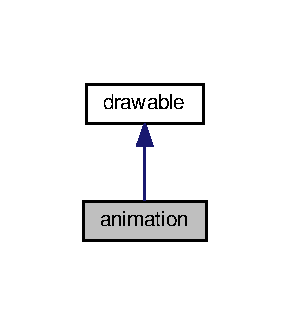
\includegraphics[width=139pt]{classanimation__inherit__graph}
\end{center}
\end{figure}


Collaboration diagram for animation\+:\nopagebreak
\begin{figure}[H]
\begin{center}
\leavevmode
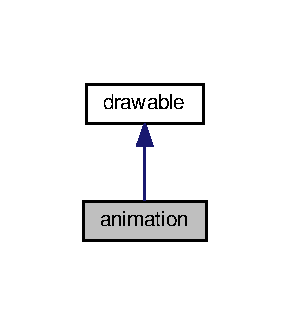
\includegraphics[width=139pt]{classanimation__coll__graph}
\end{center}
\end{figure}
\subsection*{Public Member Functions}
\begin{DoxyCompactItemize}
\item 
\hyperlink{classanimation_ab0a44a89f36d6f04c4e21e868441d693}{animation} (sf\+::\+Vector2f position, std\+::string sheet\+\_\+name)
\begin{DoxyCompactList}\small\item\em constructor \end{DoxyCompactList}\item 
void \hyperlink{classanimation_a20959b66d1c25007890bb40f0e876570}{draw} (sf\+::\+Render\+Window \&window) override
\begin{DoxyCompactList}\small\item\em draw object \end{DoxyCompactList}\item 
sf\+::\+Float\+Rect \hyperlink{classanimation_aae3322323bf3dea83723969f364e18e0}{get\+Global\+Bounds} () override
\begin{DoxyCompactList}\small\item\em get objects floatrect \end{DoxyCompactList}\item 
void \hyperlink{classanimation_ac461adb38b8241427150c4620ee31358}{set\+\_\+position} (sf\+::\+Vector2f new\+\_\+position)
\begin{DoxyCompactList}\small\item\em set position \end{DoxyCompactList}\item 
void \hyperlink{classanimation_a7c0b874294e81f3612590920fd845602}{set\+\_\+size} (sf\+::\+Vector2f new\+\_\+size)
\begin{DoxyCompactList}\small\item\em set size \end{DoxyCompactList}\item 
bool \hyperlink{classanimation_a79260eb98a4f77aa4b9f3b08cc8e5b59}{movement} (float row\+\_\+a)
\begin{DoxyCompactList}\small\item\em This function for animations. \end{DoxyCompactList}\item 
void \hyperlink{classanimation_a30e84ff71206b8ec4f82fd70ad776036}{set\+Texture\+Rect} (const sf\+::\+Int\+Rect \&rectangle)
\begin{DoxyCompactList}\small\item\em set the texture rectangle \end{DoxyCompactList}\end{DoxyCompactItemize}
\subsection*{Additional Inherited Members}


\subsection{Detailed Description}
create sprite on screen with animations 

This class creates an sprite with an image as texture. The image contains all needed images for the animations of that object.

\begin{DoxySeeAlso}{See also}
\hyperlink{classdrawable}{drawable} 

\href{https://www.sfml-dev.org/documentation/2.0/classsf_1_1Sprite.php }{\tt sf\+::\+Sprite} 

\href{https://www.sfml-dev.org/documentation/2.0/classsf_1_1Texture.php}{\tt sf\+::\+Texture} 
\end{DoxySeeAlso}


\subsection{Constructor \& Destructor Documentation}
\mbox{\Hypertarget{classanimation_ab0a44a89f36d6f04c4e21e868441d693}\label{classanimation_ab0a44a89f36d6f04c4e21e868441d693}} 
\index{animation@{animation}!animation@{animation}}
\index{animation@{animation}!animation@{animation}}
\subsubsection{\texorpdfstring{animation()}{animation()}}
{\footnotesize\ttfamily animation\+::animation (\begin{DoxyParamCaption}\item[{sf\+::\+Vector2f}]{position,  }\item[{std\+::string}]{sheet\+\_\+name }\end{DoxyParamCaption})}



constructor 

The constructor tries to load an sheet with the sheet name specified. If it can not load the image it generates an exception that can be caught with an try, catch block.


\begin{DoxyParams}[1]{Parameters}
\mbox{\tt in}  & {\em position} & The objects initial position \\
\hline
\mbox{\tt in}  & {\em image\+\_\+name} & The name of the image that has to be loaded \\
\hline
\end{DoxyParams}
\begin{DoxySeeAlso}{See also}
\hyperlink{classsheet__load__error}{sheet\+\_\+load\+\_\+error} 
\end{DoxySeeAlso}
\begin{DoxyWarning}{Warning}
Make sure you use a Try catch block to capture the exception generated if the image cannot be loaded 
\end{DoxyWarning}


\subsection{Member Function Documentation}
\mbox{\Hypertarget{classanimation_a20959b66d1c25007890bb40f0e876570}\label{classanimation_a20959b66d1c25007890bb40f0e876570}} 
\index{animation@{animation}!draw@{draw}}
\index{draw@{draw}!animation@{animation}}
\subsubsection{\texorpdfstring{draw()}{draw()}}
{\footnotesize\ttfamily void animation\+::draw (\begin{DoxyParamCaption}\item[{sf\+::\+Render\+Window \&}]{window }\end{DoxyParamCaption})\hspace{0.3cm}{\ttfamily [override]}, {\ttfamily [virtual]}}



draw object 

This function is used for calling the draw function on the sfml object created within this class. It also sets the position for before it draws the object. This way if the position changes, it also changes on screen.


\begin{DoxyParams}[1]{Parameters}
\mbox{\tt in,out}  & {\em window} & The render window to draw the object on \\
\hline
\end{DoxyParams}


Implements \hyperlink{classdrawable_a4e49e2c1121704c83ce24c5f48dd910f}{drawable}.

\mbox{\Hypertarget{classanimation_aae3322323bf3dea83723969f364e18e0}\label{classanimation_aae3322323bf3dea83723969f364e18e0}} 
\index{animation@{animation}!get\+Global\+Bounds@{get\+Global\+Bounds}}
\index{get\+Global\+Bounds@{get\+Global\+Bounds}!animation@{animation}}
\subsubsection{\texorpdfstring{get\+Global\+Bounds()}{getGlobalBounds()}}
{\footnotesize\ttfamily sf\+::\+Float\+Rect animation\+::get\+Global\+Bounds (\begin{DoxyParamCaption}{ }\end{DoxyParamCaption})\hspace{0.3cm}{\ttfamily [override]}, {\ttfamily [virtual]}}



get objects floatrect 

This function uses the get\+Global\+Bounds function from te object to get the bounding box of the object. It returns this as a floatrect. This return value can be used to check if the object touches another object.


\begin{DoxyParams}[1]{Parameters}
\mbox{\tt in}  & {\em position} & The objects initial position \\
\hline
\mbox{\tt in}  & {\em image\+\_\+name} & The name of the image that has to be loaded \\
\hline
\end{DoxyParams}

\begin{DoxyRetVals}{Return values}
{\em sf\+::\+Float\+Rect} & \{The bounding box of the sprite object created in this class\} \\
\hline
\end{DoxyRetVals}


Implements \hyperlink{classdrawable_ae013ac0be47538be9ce885d6642daf73}{drawable}.

\mbox{\Hypertarget{classanimation_a79260eb98a4f77aa4b9f3b08cc8e5b59}\label{classanimation_a79260eb98a4f77aa4b9f3b08cc8e5b59}} 
\index{animation@{animation}!movement@{movement}}
\index{movement@{movement}!animation@{animation}}
\subsubsection{\texorpdfstring{movement()}{movement()}}
{\footnotesize\ttfamily bool animation\+::movement (\begin{DoxyParamCaption}\item[{float}]{row\+\_\+a }\end{DoxyParamCaption})}



This function for animations. 


\begin{DoxyParams}[1]{Parameters}
\mbox{\tt in}  & {\em row\+\_\+a} & int indicator for which animation is needed \\
\hline
\end{DoxyParams}
\mbox{\Hypertarget{classanimation_ac461adb38b8241427150c4620ee31358}\label{classanimation_ac461adb38b8241427150c4620ee31358}} 
\index{animation@{animation}!set\+\_\+position@{set\+\_\+position}}
\index{set\+\_\+position@{set\+\_\+position}!animation@{animation}}
\subsubsection{\texorpdfstring{set\+\_\+position()}{set\_position()}}
{\footnotesize\ttfamily void animation\+::set\+\_\+position (\begin{DoxyParamCaption}\item[{sf\+::\+Vector2f}]{new\+\_\+position }\end{DoxyParamCaption})}



set position 

This function sets the position of the object to a new value.


\begin{DoxyParams}[1]{Parameters}
\mbox{\tt in}  & {\em new\+\_\+position} & sf\+::\+Vector2f The position we want to move the object to \\
\hline
\end{DoxyParams}
\begin{DoxySeeAlso}{See also}
\href{https://www.sfml-dev.org/documentation/2.0/classsf_1_1Vector2.php }{\tt sf\+::\+Vector2f} 
\end{DoxySeeAlso}
\mbox{\Hypertarget{classanimation_a7c0b874294e81f3612590920fd845602}\label{classanimation_a7c0b874294e81f3612590920fd845602}} 
\index{animation@{animation}!set\+\_\+size@{set\+\_\+size}}
\index{set\+\_\+size@{set\+\_\+size}!animation@{animation}}
\subsubsection{\texorpdfstring{set\+\_\+size()}{set\_size()}}
{\footnotesize\ttfamily void animation\+::set\+\_\+size (\begin{DoxyParamCaption}\item[{sf\+::\+Vector2f}]{new\+\_\+size }\end{DoxyParamCaption})}



set size 

This function sets the size of the object.


\begin{DoxyParams}[1]{Parameters}
\mbox{\tt in}  & {\em new\+\_\+size} & sf\+::\+Vector2f The size we want to set the object to \\
\hline
\end{DoxyParams}
\begin{DoxySeeAlso}{See also}
\href{https://www.sfml-dev.org/documentation/2.0/classsf_1_1Vector2.php }{\tt sf\+::\+Vector2f} 
\end{DoxySeeAlso}
\mbox{\Hypertarget{classanimation_a30e84ff71206b8ec4f82fd70ad776036}\label{classanimation_a30e84ff71206b8ec4f82fd70ad776036}} 
\index{animation@{animation}!set\+Texture\+Rect@{set\+Texture\+Rect}}
\index{set\+Texture\+Rect@{set\+Texture\+Rect}!animation@{animation}}
\subsubsection{\texorpdfstring{set\+Texture\+Rect()}{setTextureRect()}}
{\footnotesize\ttfamily void animation\+::set\+Texture\+Rect (\begin{DoxyParamCaption}\item[{const sf\+::\+Int\+Rect \&}]{rectangle }\end{DoxyParamCaption})}



set the texture rectangle 

This function can be used to turn the object around while keeping the same upper left corner as the position of the object.


\begin{DoxyParams}[1]{Parameters}
\mbox{\tt in}  & {\em rectangle} & const sf\+::\+Int\+Rect\& The rectangle box to turn around \\
\hline
\end{DoxyParams}
\begin{DoxySeeAlso}{See also}
\href{https://www.sfml-dev.org/documentation/2.0/classsf_1_1Sprite.php#a3fefec419a4e6a90c0fd54c793d82ec2 }{\tt sf\+::\+Sprite\+::set\+Texture\+Rect sf\+::\+Int\+Rect} 
\end{DoxySeeAlso}


The documentation for this class was generated from the following files\+:\begin{DoxyCompactItemize}
\item 
\hyperlink{animation_8hpp}{animation.\+hpp}\item 
animation.\+cpp\end{DoxyCompactItemize}

\hypertarget{classaudio__load__error}{}\section{audio\+\_\+load\+\_\+error Class Reference}
\label{classaudio__load__error}\index{audio\+\_\+load\+\_\+error@{audio\+\_\+load\+\_\+error}}


\hyperlink{classaudio__load__error}{audio\+\_\+load\+\_\+error}  




{\ttfamily \#include $<$exceptions.\+hpp$>$}



Inheritance diagram for audio\+\_\+load\+\_\+error\+:\nopagebreak
\begin{figure}[H]
\begin{center}
\leavevmode
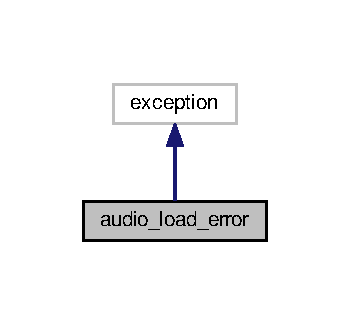
\includegraphics[width=168pt]{classaudio__load__error__inherit__graph}
\end{center}
\end{figure}


Collaboration diagram for audio\+\_\+load\+\_\+error\+:\nopagebreak
\begin{figure}[H]
\begin{center}
\leavevmode
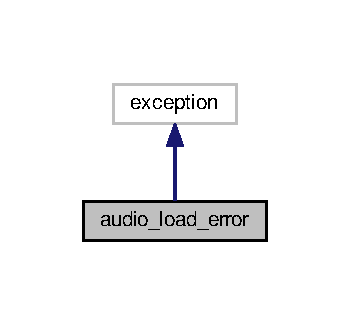
\includegraphics[width=168pt]{classaudio__load__error__coll__graph}
\end{center}
\end{figure}
\subsection*{Public Member Functions}
\begin{DoxyCompactItemize}
\item 
\hyperlink{classaudio__load__error_a6eea512cfea7b3d438afc5c1af8c63aa}{audio\+\_\+load\+\_\+error} (const std\+::string \&audio\+\_\+name)
\begin{DoxyCompactList}\small\item\em constructor \end{DoxyCompactList}\item 
const char $\ast$ \hyperlink{classaudio__load__error_a364ad9c1cb7de37f0cb3e33dbebbaa47}{what} () const noexcept override
\begin{DoxyCompactList}\small\item\em return message \end{DoxyCompactList}\end{DoxyCompactItemize}
\subsection*{Private Attributes}
\begin{DoxyCompactItemize}
\item 
std\+::string \hyperlink{classaudio__load__error_a95628dfb2fb03d93f2864a7e87cf7e79}{msg}
\end{DoxyCompactItemize}


\subsection{Detailed Description}
\hyperlink{classaudio__load__error}{audio\+\_\+load\+\_\+error} 

This class is used to generate a audio load error exception. It inherrits the std\+::exception class so it can be easily caught with an try catch block.

\begin{DoxyDate}{Date}
24-\/1-\/2017 
\end{DoxyDate}


\subsection{Constructor \& Destructor Documentation}
\mbox{\Hypertarget{classaudio__load__error_a6eea512cfea7b3d438afc5c1af8c63aa}\label{classaudio__load__error_a6eea512cfea7b3d438afc5c1af8c63aa}} 
\index{audio\+\_\+load\+\_\+error@{audio\+\_\+load\+\_\+error}!audio\+\_\+load\+\_\+error@{audio\+\_\+load\+\_\+error}}
\index{audio\+\_\+load\+\_\+error@{audio\+\_\+load\+\_\+error}!audio\+\_\+load\+\_\+error@{audio\+\_\+load\+\_\+error}}
\subsubsection{\texorpdfstring{audio\+\_\+load\+\_\+error()}{audio\_load\_error()}}
{\footnotesize\ttfamily audio\+\_\+load\+\_\+error\+::audio\+\_\+load\+\_\+error (\begin{DoxyParamCaption}\item[{const std\+::string \&}]{audio\+\_\+name }\end{DoxyParamCaption})\hspace{0.3cm}{\ttfamily [inline]}}



constructor 

This constructor puts a message into a string and saves that as a private variable. The audio name is also added to the string.


\begin{DoxyParams}[1]{Parameters}
\mbox{\tt in}  & {\em load\+\_\+name} & The name of the image \\
\hline
\end{DoxyParams}


\subsection{Member Function Documentation}
\mbox{\Hypertarget{classaudio__load__error_a364ad9c1cb7de37f0cb3e33dbebbaa47}\label{classaudio__load__error_a364ad9c1cb7de37f0cb3e33dbebbaa47}} 
\index{audio\+\_\+load\+\_\+error@{audio\+\_\+load\+\_\+error}!what@{what}}
\index{what@{what}!audio\+\_\+load\+\_\+error@{audio\+\_\+load\+\_\+error}}
\subsubsection{\texorpdfstring{what()}{what()}}
{\footnotesize\ttfamily const char$\ast$ audio\+\_\+load\+\_\+error\+::what (\begin{DoxyParamCaption}{ }\end{DoxyParamCaption}) const\hspace{0.3cm}{\ttfamily [inline]}, {\ttfamily [override]}, {\ttfamily [noexcept]}}



return message 

This function returns the message so it can be printed. It overrides the what function from the std\+::exception superclass, making it easy to capture.


\begin{DoxyRetVals}{Return values}
{\em const} & char $\ast$ \{The error message as a const char $\ast$\} \\
\hline
\end{DoxyRetVals}


\subsection{Member Data Documentation}
\mbox{\Hypertarget{classaudio__load__error_a95628dfb2fb03d93f2864a7e87cf7e79}\label{classaudio__load__error_a95628dfb2fb03d93f2864a7e87cf7e79}} 
\index{audio\+\_\+load\+\_\+error@{audio\+\_\+load\+\_\+error}!msg@{msg}}
\index{msg@{msg}!audio\+\_\+load\+\_\+error@{audio\+\_\+load\+\_\+error}}
\subsubsection{\texorpdfstring{msg}{msg}}
{\footnotesize\ttfamily std\+::string audio\+\_\+load\+\_\+error\+::msg\hspace{0.3cm}{\ttfamily [private]}}



The documentation for this class was generated from the following file\+:\begin{DoxyCompactItemize}
\item 
\hyperlink{exceptions_8hpp}{exceptions.\+hpp}\end{DoxyCompactItemize}

\hypertarget{classbackground}{}\section{background Class Reference}
\label{classbackground}\index{background@{background}}


{\ttfamily \#include $<$background.\+hpp$>$}



Inheritance diagram for background\+:\nopagebreak
\begin{figure}[H]
\begin{center}
\leavevmode
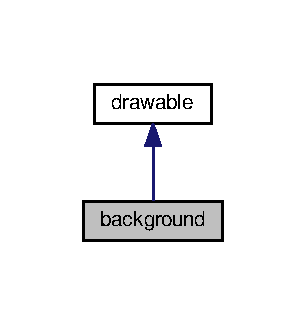
\includegraphics[width=147pt]{classbackground__inherit__graph}
\end{center}
\end{figure}


Collaboration diagram for background\+:\nopagebreak
\begin{figure}[H]
\begin{center}
\leavevmode
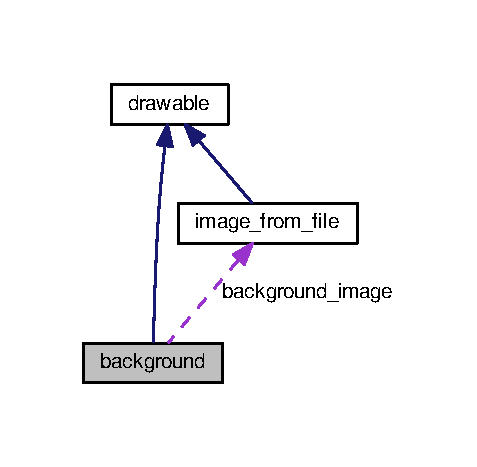
\includegraphics[width=229pt]{classbackground__coll__graph}
\end{center}
\end{figure}
\subsection*{Public Member Functions}
\begin{DoxyCompactItemize}
\item 
\hyperlink{classbackground_ad199eead2ef4a4d867f2542d3a152471}{background} (std\+::string filename, sf\+::\+Vector2f level\+\_\+size)
\begin{DoxyCompactList}\small\item\em constructor for background class \end{DoxyCompactList}\item 
void \hyperlink{classbackground_a41736f9a00defad1e84b3a8099c887e2}{draw} (sf\+::\+Render\+Window \&window) override
\begin{DoxyCompactList}\small\item\em Draw function for background class. \end{DoxyCompactList}\item 
sf\+::\+Float\+Rect \hyperlink{classbackground_ab5f2b627cd58e0d07678f0af01c6bd2d}{get\+Global\+Bounds} () override
\begin{DoxyCompactList}\small\item\em Get the global bounds. \end{DoxyCompactList}\end{DoxyCompactItemize}
\subsection*{Private Attributes}
\begin{DoxyCompactItemize}
\item 
\hyperlink{classimage__from__file}{image\+\_\+from\+\_\+file} \hyperlink{classbackground_a972ef28e3ac5aea925fc9d00e809d5af}{background\+\_\+image}
\end{DoxyCompactItemize}
\subsection*{Additional Inherited Members}


\subsection{Constructor \& Destructor Documentation}
\mbox{\Hypertarget{classbackground_ad199eead2ef4a4d867f2542d3a152471}\label{classbackground_ad199eead2ef4a4d867f2542d3a152471}} 
\index{background@{background}!background@{background}}
\index{background@{background}!background@{background}}
\subsubsection{\texorpdfstring{background()}{background()}}
{\footnotesize\ttfamily background\+::background (\begin{DoxyParamCaption}\item[{std\+::string}]{filename,  }\item[{sf\+::\+Vector2f}]{level\+\_\+size }\end{DoxyParamCaption})}



constructor for background class 

constructor that initializes the file that the background class will use. Default is \char`\"{}x\char`\"{}, if default a default picture will be loaded.


\begin{DoxyParams}[1]{Parameters}
\mbox{\tt in}  & {\em std\+::string} & name of the .png file that will be loaded as a background \\
\hline
\end{DoxyParams}


\subsection{Member Function Documentation}
\mbox{\Hypertarget{classbackground_a41736f9a00defad1e84b3a8099c887e2}\label{classbackground_a41736f9a00defad1e84b3a8099c887e2}} 
\index{background@{background}!draw@{draw}}
\index{draw@{draw}!background@{background}}
\subsubsection{\texorpdfstring{draw()}{draw()}}
{\footnotesize\ttfamily void background\+::draw (\begin{DoxyParamCaption}\item[{sf\+::\+Render\+Window \&}]{window }\end{DoxyParamCaption})\hspace{0.3cm}{\ttfamily [override]}, {\ttfamily [virtual]}}



Draw function for background class. 

defines draw function in super class. Draws the background.


\begin{DoxyParams}[1]{Parameters}
\mbox{\tt in}  & {\em window} & S\+F\+ML window that is used to display the drawable \\
\hline
\end{DoxyParams}


Implements \hyperlink{classdrawable_a4e49e2c1121704c83ce24c5f48dd910f}{drawable}.

\mbox{\Hypertarget{classbackground_ab5f2b627cd58e0d07678f0af01c6bd2d}\label{classbackground_ab5f2b627cd58e0d07678f0af01c6bd2d}} 
\index{background@{background}!get\+Global\+Bounds@{get\+Global\+Bounds}}
\index{get\+Global\+Bounds@{get\+Global\+Bounds}!background@{background}}
\subsubsection{\texorpdfstring{get\+Global\+Bounds()}{getGlobalBounds()}}
{\footnotesize\ttfamily sf\+::\+Float\+Rect background\+::get\+Global\+Bounds (\begin{DoxyParamCaption}{ }\end{DoxyParamCaption})\hspace{0.3cm}{\ttfamily [override]}, {\ttfamily [virtual]}}



Get the global bounds. 

This function returns the global bounds of the \hyperlink{classbackground_a972ef28e3ac5aea925fc9d00e809d5af}{background\+\_\+image}. Those global bounds can be used for things like checking collisions. \begin{DoxyReturn}{Returns}
The global bounds of the \hyperlink{classbackground_a972ef28e3ac5aea925fc9d00e809d5af}{background\+\_\+image} 
\end{DoxyReturn}


Implements \hyperlink{classdrawable_ae013ac0be47538be9ce885d6642daf73}{drawable}.



\subsection{Member Data Documentation}
\mbox{\Hypertarget{classbackground_a972ef28e3ac5aea925fc9d00e809d5af}\label{classbackground_a972ef28e3ac5aea925fc9d00e809d5af}} 
\index{background@{background}!background\+\_\+image@{background\+\_\+image}}
\index{background\+\_\+image@{background\+\_\+image}!background@{background}}
\subsubsection{\texorpdfstring{background\+\_\+image}{background\_image}}
{\footnotesize\ttfamily \hyperlink{classimage__from__file}{image\+\_\+from\+\_\+file} background\+::background\+\_\+image\hspace{0.3cm}{\ttfamily [private]}}



The documentation for this class was generated from the following files\+:\begin{DoxyCompactItemize}
\item 
\hyperlink{background_8hpp}{background.\+hpp}\item 
\hyperlink{background_8cpp}{background.\+cpp}\end{DoxyCompactItemize}

\hypertarget{classbase__level}{}\section{base\+\_\+level Class Reference}
\label{classbase__level}\index{base\+\_\+level@{base\+\_\+level}}


{\ttfamily \#include $<$base\+\_\+level.\+hpp$>$}

\subsection*{Public Member Functions}
\begin{DoxyCompactItemize}
\item 
\hyperlink{classbase__level_addf165fdc5f4e953be3b6a2dcd00459b}{base\+\_\+level} (sf\+::\+Vector2f \hyperlink{classbase__level_a69702ca202fa2a3a4c83faaa807971c2}{screen\+\_\+size})
\begin{DoxyCompactList}\small\item\em constructor screen size \end{DoxyCompactList}\item 
void \hyperlink{classbase__level_a3b2da28cf45cad434103e81ee6c4538d}{push\+\_\+back\+\_\+borders} (\hyperlink{drawable_8hpp_a6c0fdb1dfd0c34dbbdbb5dcd3c608b07}{objects\+\_\+vector} \&objects)
\begin{DoxyCompactList}\small\item\em Put walls in the walls vector. \end{DoxyCompactList}\end{DoxyCompactItemize}
\subsection*{Private Attributes}
\begin{DoxyCompactItemize}
\item 
sf\+::\+Vector2f \hyperlink{classbase__level_a69702ca202fa2a3a4c83faaa807971c2}{screen\+\_\+size}
\item 
\hyperlink{drawable_8hpp_aab5add95f06d2ba25dbfed8eb07274fa}{object\+\_\+ptr} \hyperlink{classbase__level_a196474637fdc953f4f2ed088ace891f7}{lower\+\_\+wall}
\item 
\hyperlink{drawable_8hpp_aab5add95f06d2ba25dbfed8eb07274fa}{object\+\_\+ptr} \hyperlink{classbase__level_a4a1f6a57a83aec4bd0b82072ab21df43}{right\+\_\+wall}
\item 
\hyperlink{drawable_8hpp_aab5add95f06d2ba25dbfed8eb07274fa}{object\+\_\+ptr} \hyperlink{classbase__level_a5e4ab9bce71cb388025305d0f20cb7bf}{upper\+\_\+wall}
\item 
\hyperlink{drawable_8hpp_aab5add95f06d2ba25dbfed8eb07274fa}{object\+\_\+ptr} \hyperlink{classbase__level_a29e885695d2a043bdab849dcb73c5c8e}{left\+\_\+wall}
\end{DoxyCompactItemize}


\subsection{Constructor \& Destructor Documentation}
\mbox{\Hypertarget{classbase__level_addf165fdc5f4e953be3b6a2dcd00459b}\label{classbase__level_addf165fdc5f4e953be3b6a2dcd00459b}} 
\index{base\+\_\+level@{base\+\_\+level}!base\+\_\+level@{base\+\_\+level}}
\index{base\+\_\+level@{base\+\_\+level}!base\+\_\+level@{base\+\_\+level}}
\subsubsection{\texorpdfstring{base\+\_\+level()}{base\_level()}}
{\footnotesize\ttfamily base\+\_\+level\+::base\+\_\+level (\begin{DoxyParamCaption}\item[{sf\+::\+Vector2f}]{screen\+\_\+size }\end{DoxyParamCaption})}



constructor screen size 

This constructor receives the screen size and creates all the walls with the right sizes. It makes them transparent to make sure you can not see the screen borders. It also changes the type of the wall objects to make sure other objects can know that they are not regular wall objects but of a special type. 
\begin{DoxyParams}[1]{Parameters}
\mbox{\tt in}  & {\em screen\+\_\+size} & The size of the screen \\
\hline
\end{DoxyParams}


\subsection{Member Function Documentation}
\mbox{\Hypertarget{classbase__level_a3b2da28cf45cad434103e81ee6c4538d}\label{classbase__level_a3b2da28cf45cad434103e81ee6c4538d}} 
\index{base\+\_\+level@{base\+\_\+level}!push\+\_\+back\+\_\+borders@{push\+\_\+back\+\_\+borders}}
\index{push\+\_\+back\+\_\+borders@{push\+\_\+back\+\_\+borders}!base\+\_\+level@{base\+\_\+level}}
\subsubsection{\texorpdfstring{push\+\_\+back\+\_\+borders()}{push\_back\_borders()}}
{\footnotesize\ttfamily void base\+\_\+level\+::push\+\_\+back\+\_\+borders (\begin{DoxyParamCaption}\item[{\hyperlink{drawable_8hpp_a6c0fdb1dfd0c34dbbdbb5dcd3c608b07}{objects\+\_\+vector} \&}]{objects }\end{DoxyParamCaption})}



Put walls in the walls vector. 

This function puts the level borders in the vector with all the wall objects. This makes sure they are drawn. 
\begin{DoxyParams}[1]{Parameters}
\mbox{\tt in}  & {\em objects} & The vector with al the other wall objects \\
\hline
\end{DoxyParams}


\subsection{Member Data Documentation}
\mbox{\Hypertarget{classbase__level_a29e885695d2a043bdab849dcb73c5c8e}\label{classbase__level_a29e885695d2a043bdab849dcb73c5c8e}} 
\index{base\+\_\+level@{base\+\_\+level}!left\+\_\+wall@{left\+\_\+wall}}
\index{left\+\_\+wall@{left\+\_\+wall}!base\+\_\+level@{base\+\_\+level}}
\subsubsection{\texorpdfstring{left\+\_\+wall}{left\_wall}}
{\footnotesize\ttfamily \hyperlink{drawable_8hpp_aab5add95f06d2ba25dbfed8eb07274fa}{object\+\_\+ptr} base\+\_\+level\+::left\+\_\+wall\hspace{0.3cm}{\ttfamily [private]}}

\mbox{\Hypertarget{classbase__level_a196474637fdc953f4f2ed088ace891f7}\label{classbase__level_a196474637fdc953f4f2ed088ace891f7}} 
\index{base\+\_\+level@{base\+\_\+level}!lower\+\_\+wall@{lower\+\_\+wall}}
\index{lower\+\_\+wall@{lower\+\_\+wall}!base\+\_\+level@{base\+\_\+level}}
\subsubsection{\texorpdfstring{lower\+\_\+wall}{lower\_wall}}
{\footnotesize\ttfamily \hyperlink{drawable_8hpp_aab5add95f06d2ba25dbfed8eb07274fa}{object\+\_\+ptr} base\+\_\+level\+::lower\+\_\+wall\hspace{0.3cm}{\ttfamily [private]}}

\mbox{\Hypertarget{classbase__level_a4a1f6a57a83aec4bd0b82072ab21df43}\label{classbase__level_a4a1f6a57a83aec4bd0b82072ab21df43}} 
\index{base\+\_\+level@{base\+\_\+level}!right\+\_\+wall@{right\+\_\+wall}}
\index{right\+\_\+wall@{right\+\_\+wall}!base\+\_\+level@{base\+\_\+level}}
\subsubsection{\texorpdfstring{right\+\_\+wall}{right\_wall}}
{\footnotesize\ttfamily \hyperlink{drawable_8hpp_aab5add95f06d2ba25dbfed8eb07274fa}{object\+\_\+ptr} base\+\_\+level\+::right\+\_\+wall\hspace{0.3cm}{\ttfamily [private]}}

\mbox{\Hypertarget{classbase__level_a69702ca202fa2a3a4c83faaa807971c2}\label{classbase__level_a69702ca202fa2a3a4c83faaa807971c2}} 
\index{base\+\_\+level@{base\+\_\+level}!screen\+\_\+size@{screen\+\_\+size}}
\index{screen\+\_\+size@{screen\+\_\+size}!base\+\_\+level@{base\+\_\+level}}
\subsubsection{\texorpdfstring{screen\+\_\+size}{screen\_size}}
{\footnotesize\ttfamily sf\+::\+Vector2f base\+\_\+level\+::screen\+\_\+size\hspace{0.3cm}{\ttfamily [private]}}

\mbox{\Hypertarget{classbase__level_a5e4ab9bce71cb388025305d0f20cb7bf}\label{classbase__level_a5e4ab9bce71cb388025305d0f20cb7bf}} 
\index{base\+\_\+level@{base\+\_\+level}!upper\+\_\+wall@{upper\+\_\+wall}}
\index{upper\+\_\+wall@{upper\+\_\+wall}!base\+\_\+level@{base\+\_\+level}}
\subsubsection{\texorpdfstring{upper\+\_\+wall}{upper\_wall}}
{\footnotesize\ttfamily \hyperlink{drawable_8hpp_aab5add95f06d2ba25dbfed8eb07274fa}{object\+\_\+ptr} base\+\_\+level\+::upper\+\_\+wall\hspace{0.3cm}{\ttfamily [private]}}



The documentation for this class was generated from the following files\+:\begin{DoxyCompactItemize}
\item 
\hyperlink{base__level_8hpp}{base\+\_\+level.\+hpp}\item 
\hyperlink{base__level_8cpp}{base\+\_\+level.\+cpp}\end{DoxyCompactItemize}

\hypertarget{classbullet}{}\section{bullet Class Reference}
\label{classbullet}\index{bullet@{bullet}}


class calculates projectile to kill mobs  




{\ttfamily \#include $<$bullet.\+hpp$>$}



Inheritance diagram for bullet\+:\nopagebreak
\begin{figure}[H]
\begin{center}
\leavevmode
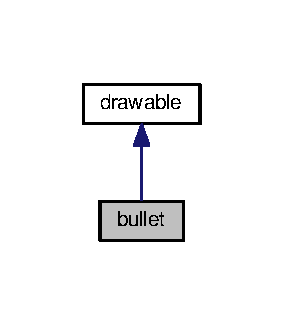
\includegraphics[width=136pt]{classbullet__inherit__graph}
\end{center}
\end{figure}


Collaboration diagram for bullet\+:\nopagebreak
\begin{figure}[H]
\begin{center}
\leavevmode
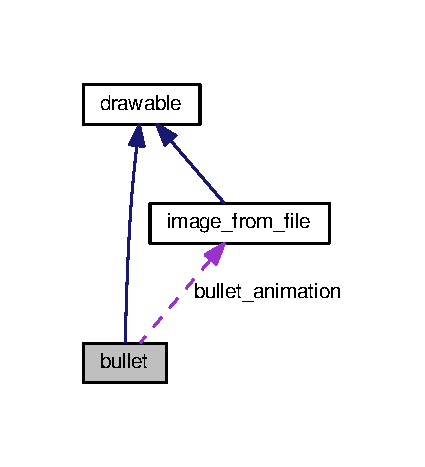
\includegraphics[width=136pt]{classbullet__coll__graph}
\end{center}
\end{figure}
\subsection*{Public Member Functions}
\begin{DoxyCompactItemize}
\item 
\hyperlink{classbullet_a2c8b1e868ab8fe8edf43fc289f8d80b8}{bullet} (sf\+::\+Vector2f position, std\+::string filename, std\+::vector$<$ mob\+\_\+ptr $>$ \&all\+\_\+mobs, objects\+\_\+vector \&objects)
\begin{DoxyCompactList}\small\item\em constructor to initialize the bullet \end{DoxyCompactList}\item 
void \hyperlink{classbullet_ae999b952538687d45ca2ae54164a5cd8}{draw} (sf\+::\+Render\+Window \&window) override
\begin{DoxyCompactList}\small\item\em funtion that draws image \end{DoxyCompactList}\item 
sf\+::\+Float\+Rect \hyperlink{classbullet_a87bda5887249e8e37c5579180449bd93}{get\+Global\+Bounds} () override
\begin{DoxyCompactList}\small\item\em function that gets the globalbounds of the bullet\+\_\+animation \end{DoxyCompactList}\item 
{\footnotesize template$<$typename P $>$ }\\void \hyperlink{classbullet_ab7e5c677bbd642df24a2251bb58249b7}{collision} (P unique\+\_\+object)
\begin{DoxyCompactList}\small\item\em function that checks collision with pointer \end{DoxyCompactList}\item 
void \hyperlink{classbullet_a52d736cad2a486a65c8a25781cff1f70}{shoot} (sf\+::\+Render\+Window \&window, int \&shoot\+\_\+timeout, sf\+::\+Vector2f offset=sf\+::\+Vector2f(0, 0), sf\+::\+Vector2f fire\+\_\+position=sf\+::\+Vector2f(0.\+0, 0.\+0))
\begin{DoxyCompactList}\small\item\em function that manages moving the bullet and checking for collision \end{DoxyCompactList}\item 
\mbox{\Hypertarget{classbullet_af338da31bfb1dd4b2d942ca67316350a}\label{classbullet_af338da31bfb1dd4b2d942ca67316350a}} 
void {\bfseries set\+\_\+position} (sf\+::\+Vector2f new\+\_\+position)
\end{DoxyCompactItemize}
\subsection*{Additional Inherited Members}


\subsection{Detailed Description}
class calculates projectile to kill mobs 

This class is used to calculate a projectile that can kill mobs (if there hit by the object)

\begin{DoxyDate}{Date}
26-\/01-\/2017 
\end{DoxyDate}


\subsection{Constructor \& Destructor Documentation}
\mbox{\Hypertarget{classbullet_a2c8b1e868ab8fe8edf43fc289f8d80b8}\label{classbullet_a2c8b1e868ab8fe8edf43fc289f8d80b8}} 
\index{bullet@{bullet}!bullet@{bullet}}
\index{bullet@{bullet}!bullet@{bullet}}
\subsubsection{\texorpdfstring{bullet()}{bullet()}}
{\footnotesize\ttfamily bullet\+::bullet (\begin{DoxyParamCaption}\item[{sf\+::\+Vector2f}]{position,  }\item[{std\+::string}]{filename,  }\item[{std\+::vector$<$ mob\+\_\+ptr $>$ \&}]{all\+\_\+mobs,  }\item[{objects\+\_\+vector \&}]{objects }\end{DoxyParamCaption})}



constructor to initialize the bullet 

This constructor intializes the position and picture used for the bullet. It also receives two std\+::vectors, one vector for all mobs in the level, the other for all walls in the level


\begin{DoxyParams}[1]{Parameters}
\mbox{\tt in}  & {\em position} & sf\+::\+Vector2f position where the bullet is placed \\
\hline
\mbox{\tt in}  & {\em filename} & std\+::string that is the filename of the image used \\
\hline
\mbox{\tt in}  & {\em all\+\_\+mobs} & std\+::vector with mob shared\+\_\+pointers to all mobs in the level \\
\hline
\mbox{\tt in}  & {\em objects} & std\+::vector with drawable shared\+\_\+pointers to all walls/obstacles in the level \\
\hline
\end{DoxyParams}


\subsection{Member Function Documentation}
\mbox{\Hypertarget{classbullet_ab7e5c677bbd642df24a2251bb58249b7}\label{classbullet_ab7e5c677bbd642df24a2251bb58249b7}} 
\index{bullet@{bullet}!collision@{collision}}
\index{collision@{collision}!bullet@{bullet}}
\subsubsection{\texorpdfstring{collision()}{collision()}}
{\footnotesize\ttfamily template$<$typename P $>$ \\
void bullet\+::collision (\begin{DoxyParamCaption}\item[{P}]{unique\+\_\+object }\end{DoxyParamCaption})}



function that checks collision with pointer 

This function checks if there is collision with either a mob or a wall and sets the boolean hit on true when collision with given object is found otherwide hit is set to false


\begin{DoxyParams}[1]{Parameters}
\mbox{\tt in}  & {\em unique\+\_\+object} & shared\+\_\+pointer or pointer that gives location of object that contains a get\+Global\+Bounds function \\
\hline
\end{DoxyParams}
\mbox{\Hypertarget{classbullet_ae999b952538687d45ca2ae54164a5cd8}\label{classbullet_ae999b952538687d45ca2ae54164a5cd8}} 
\index{bullet@{bullet}!draw@{draw}}
\index{draw@{draw}!bullet@{bullet}}
\subsubsection{\texorpdfstring{draw()}{draw()}}
{\footnotesize\ttfamily void bullet\+::draw (\begin{DoxyParamCaption}\item[{sf\+::\+Render\+Window \&}]{window }\end{DoxyParamCaption})\hspace{0.3cm}{\ttfamily [override]}, {\ttfamily [virtual]}}



funtion that draws image 

This function draws the bullet. This function checkes if the bullet is correctly scaled depending on the direction it is fired. It only draws the bullet when boolean hit is false this happens when a bullet hasn\textquotesingle{}t hit a object.


\begin{DoxyParams}[1]{Parameters}
\mbox{\tt in}  & {\em window} & sf\+::\+Renderwindow that is used to display the window on \\
\hline
\end{DoxyParams}


Implements \hyperlink{classdrawable_a4e49e2c1121704c83ce24c5f48dd910f}{drawable}.

\mbox{\Hypertarget{classbullet_a87bda5887249e8e37c5579180449bd93}\label{classbullet_a87bda5887249e8e37c5579180449bd93}} 
\index{bullet@{bullet}!get\+Global\+Bounds@{get\+Global\+Bounds}}
\index{get\+Global\+Bounds@{get\+Global\+Bounds}!bullet@{bullet}}
\subsubsection{\texorpdfstring{get\+Global\+Bounds()}{getGlobalBounds()}}
{\footnotesize\ttfamily sf\+::\+Float\+Rect bullet\+::get\+Global\+Bounds (\begin{DoxyParamCaption}{ }\end{DoxyParamCaption})\hspace{0.3cm}{\ttfamily [override]}, {\ttfamily [virtual]}}



function that gets the globalbounds of the bullet\+\_\+animation 

This function gets the globalbounds of the bullet\+\_\+animation. The globalbounds is the rectangle around the image.

\begin{DoxyReturn}{Returns}
sf\+::\+Float\+Rect around the image 
\end{DoxyReturn}


Implements \hyperlink{classdrawable_ae013ac0be47538be9ce885d6642daf73}{drawable}.

\mbox{\Hypertarget{classbullet_a52d736cad2a486a65c8a25781cff1f70}\label{classbullet_a52d736cad2a486a65c8a25781cff1f70}} 
\index{bullet@{bullet}!shoot@{shoot}}
\index{shoot@{shoot}!bullet@{bullet}}
\subsubsection{\texorpdfstring{shoot()}{shoot()}}
{\footnotesize\ttfamily void bullet\+::shoot (\begin{DoxyParamCaption}\item[{sf\+::\+Render\+Window \&}]{window,  }\item[{int \&}]{shoot\+\_\+timeout,  }\item[{sf\+::\+Vector2f}]{offset = {\ttfamily sf\+:\+:Vector2f(0,~0)},  }\item[{sf\+::\+Vector2f}]{fire\+\_\+position = {\ttfamily sf\+:\+:Vector2f(0.0,~0.0)} }\end{DoxyParamCaption})}



function that manages moving the bullet and checking for collision 

This function moves bullet with \#bullet\+::projectile() function and then checks for collisions with mobs and walls. If fire\+\_\+position is not entered the bullet moves from its last position. When offset is not entered it usually means the bullet is fired and still on the move in that case the current offset is used to make sure the bullet doesn\textquotesingle{}t follow the unicorn


\begin{DoxyParams}[1]{Parameters}
\mbox{\tt in}  & {\em window} & sf\+::\+Render\+Window that is used to display the bullet \\
\hline
\mbox{\tt in}  & {\em shoot\+\_\+timeout} & int given by reference that is used to reset the shot, when something hits the bullet \\
\hline
\mbox{\tt in}  & {\em offset} & sf\+::\+Vector2f for movement, has negative x-\/coordinate when fired to left side \\
\hline
\mbox{\tt in}  & {\em fire\+\_\+position} & sf\+::\+Vector2f for position for bullet to start projectile. \\
\hline
\end{DoxyParams}


The documentation for this class was generated from the following files\+:\begin{DoxyCompactItemize}
\item 
\hyperlink{bullet_8hpp}{bullet.\+hpp}\item 
bullet.\+cpp\end{DoxyCompactItemize}

\hypertarget{class_button}{}\section{Button Class Reference}
\label{class_button}\index{Button@{Button}}


Creates a button at a specific place on the screen.  




{\ttfamily \#include $<$button.\+hpp$>$}

\subsection*{Public Member Functions}
\begin{DoxyCompactItemize}
\item 
\hyperlink{class_button_a1085aea4e01df12c1400d2f2f666dda2}{Button} (float start\+HeightY=0.\+0, float start\+HeightX=0.\+0, int position=0, std\+::string Whats\+On\+The\+Button=\char`\"{} \char`\"{})
\begin{DoxyCompactList}\small\item\em constructor to make button \end{DoxyCompactList}\item 
void \hyperlink{class_button_adf65892636ea303a84e1391106ea7cb0}{draw} (sf\+::\+Render\+Window \&window)
\begin{DoxyCompactList}\small\item\em Function to draw the button \& the text. \end{DoxyCompactList}\item 
void \hyperlink{class_button_aaf14334dd0ac6a9c286aac71a765caa2}{setup} ()
\begin{DoxyCompactList}\small\item\em Function that decides what gets drawn where. \end{DoxyCompactList}\item 
sf\+::\+Float\+Rect \hyperlink{class_button_af662f717b2230477da7d4760293473d4}{get\+Global\+Bounds} ()
\begin{DoxyCompactList}\small\item\em get objects floatrect \end{DoxyCompactList}\end{DoxyCompactItemize}


\subsection{Detailed Description}
Creates a button at a specific place on the screen. 

This class is used to make a button that is placed at a certain position. Right now a lot of math is done in this class to make sure the button is in the exact middle of the screen, together with the ( adjustable ) text on the button.

Note\+: We would like to transfer all the math done in here to \hyperlink{classmenu}{menu}. However, this has low priority .

\begin{DoxyDate}{Date}
27-\/1-\/2017 
\end{DoxyDate}


\subsection{Constructor \& Destructor Documentation}
\mbox{\Hypertarget{class_button_a1085aea4e01df12c1400d2f2f666dda2}\label{class_button_a1085aea4e01df12c1400d2f2f666dda2}} 
\index{Button@{Button}!Button@{Button}}
\index{Button@{Button}!Button@{Button}}
\subsubsection{\texorpdfstring{Button()}{Button()}}
{\footnotesize\ttfamily Button\+::\+Button (\begin{DoxyParamCaption}\item[{float}]{start\+HeightY = {\ttfamily 0.0},  }\item[{float}]{start\+HeightX = {\ttfamily 0.0},  }\item[{int}]{position = {\ttfamily 0},  }\item[{std\+::string}]{Whats\+On\+The\+Button = {\ttfamily \char`\"{}~\char`\"{}} }\end{DoxyParamCaption})}



constructor to make button 

This constructor receives 2 floats to determine the start position of the button. The position determines at which of the three positions it will render according to screen size. The string is the text that will be displayed on the button.


\begin{DoxyParams}[1]{Parameters}
\mbox{\tt in}  & {\em start\+HeightY} & Starting height Y coordinate \\
\hline
\mbox{\tt in}  & {\em start\+HeightX} & Starting height X coordinate \\
\hline
\mbox{\tt in}  & {\em position} & The postion for the button ( 1 -\/ 2 -\/ 3) \\
\hline
\mbox{\tt in}  & {\em Whats\+On\+The\+Button} & std\+::string, the text on the button \\
\hline
\end{DoxyParams}


\subsection{Member Function Documentation}
\mbox{\Hypertarget{class_button_adf65892636ea303a84e1391106ea7cb0}\label{class_button_adf65892636ea303a84e1391106ea7cb0}} 
\index{Button@{Button}!draw@{draw}}
\index{draw@{draw}!Button@{Button}}
\subsubsection{\texorpdfstring{draw()}{draw()}}
{\footnotesize\ttfamily void Button\+::draw (\begin{DoxyParamCaption}\item[{sf\+::\+Render\+Window \&}]{window }\end{DoxyParamCaption})}



Function to draw the button \& the text. 

Function to draw both the button and the text on the given window.


\begin{DoxyParams}[1]{Parameters}
\mbox{\tt in}  & {\em window} & The display window \\
\hline
\end{DoxyParams}
\mbox{\Hypertarget{class_button_af662f717b2230477da7d4760293473d4}\label{class_button_af662f717b2230477da7d4760293473d4}} 
\index{Button@{Button}!get\+Global\+Bounds@{get\+Global\+Bounds}}
\index{get\+Global\+Bounds@{get\+Global\+Bounds}!Button@{Button}}
\subsubsection{\texorpdfstring{get\+Global\+Bounds()}{getGlobalBounds()}}
{\footnotesize\ttfamily sf\+::\+Float\+Rect Button\+::get\+Global\+Bounds (\begin{DoxyParamCaption}{ }\end{DoxyParamCaption})}



get objects floatrect 

This function uses the get\+Global\+Bounds function from te object to get the bounding box of the object. It returns this as a floatrect. This return value can be used to check if the object touches another object.


\begin{DoxyParams}[1]{Parameters}
\mbox{\tt in}  & {\em position} & The objects initial position \\
\hline
\mbox{\tt in}  & {\em image\+\_\+name} & The name of the image that has to be loaded \\
\hline
\end{DoxyParams}

\begin{DoxyRetVals}{Return values}
{\em sf\+::\+Float\+Rect} & \{The bounding box of the sprite object created in this class\} \\
\hline
\end{DoxyRetVals}
\mbox{\Hypertarget{class_button_aaf14334dd0ac6a9c286aac71a765caa2}\label{class_button_aaf14334dd0ac6a9c286aac71a765caa2}} 
\index{Button@{Button}!setup@{setup}}
\index{setup@{setup}!Button@{Button}}
\subsubsection{\texorpdfstring{setup()}{setup()}}
{\footnotesize\ttfamily void Button\+::setup (\begin{DoxyParamCaption}{ }\end{DoxyParamCaption})}



Function that decides what gets drawn where. 

This function decides where to draw the buttons. The purpose of all the math is to determine the place on the screen for the button, so it sits right in the middle of the screen. The draw position for the text is also adjusted for length of the given std\+::string. This is also the function that uses the position parameter to determine where the position gets drawn. 

The documentation for this class was generated from the following files\+:\begin{DoxyCompactItemize}
\item 
\hyperlink{button_8hpp}{button.\+hpp}\item 
button.\+cpp\end{DoxyCompactItemize}

\hypertarget{classcamera}{}\section{camera Class Reference}
\label{classcamera}\index{camera@{camera}}


object folowing camera  




{\ttfamily \#include $<$camera.\+hpp$>$}

\subsection*{Public Member Functions}
\begin{DoxyCompactItemize}
\item 
\hyperlink{classcamera_ac3c67027b5f4f19c6f12db7d909930b5}{camera} (\hyperlink{typedefs_8hpp_aab5add95f06d2ba25dbfed8eb07274fa}{object\+\_\+ptr} object)
\begin{DoxyCompactList}\small\item\em constructor object \end{DoxyCompactList}\item 
void \hyperlink{classcamera_a1bb99501ba67453e0ca86f3c8aef5cb1}{follow} (sf\+::\+Render\+Window \&window)
\begin{DoxyCompactList}\small\item\em folow in render window \end{DoxyCompactList}\end{DoxyCompactItemize}
\subsection*{Private Attributes}
\begin{DoxyCompactItemize}
\item 
\mbox{\Hypertarget{classcamera_a2f634677bff4e01829c2b7023e302d5b}\label{classcamera_a2f634677bff4e01829c2b7023e302d5b}} 
\hyperlink{typedefs_8hpp_aab5add95f06d2ba25dbfed8eb07274fa}{object\+\_\+ptr} {\bfseries object}
\item 
\mbox{\Hypertarget{classcamera_a9b28d8987a758688f2374fef925c3805}\label{classcamera_a9b28d8987a758688f2374fef925c3805}} 
sf\+::\+View {\bfseries player\+\_\+cam}
\end{DoxyCompactItemize}


\subsection{Detailed Description}
object folowing camera 

This class can be used to follow a specific drawable object with the camera. If the object moves the camera moves with it. 

\subsection{Constructor \& Destructor Documentation}
\mbox{\Hypertarget{classcamera_ac3c67027b5f4f19c6f12db7d909930b5}\label{classcamera_ac3c67027b5f4f19c6f12db7d909930b5}} 
\index{camera@{camera}!camera@{camera}}
\index{camera@{camera}!camera@{camera}}
\subsubsection{\texorpdfstring{camera()}{camera()}}
{\footnotesize\ttfamily camera\+::camera (\begin{DoxyParamCaption}\item[{\hyperlink{typedefs_8hpp_aab5add95f06d2ba25dbfed8eb07274fa}{object\+\_\+ptr}}]{object }\end{DoxyParamCaption})}



constructor object 

Constructor to make a camera that follows the player.


\begin{DoxyParams}[1]{Parameters}
\mbox{\tt in}  & {\em object} & The object to follow \\
\hline
\end{DoxyParams}


\subsection{Member Function Documentation}
\mbox{\Hypertarget{classcamera_a1bb99501ba67453e0ca86f3c8aef5cb1}\label{classcamera_a1bb99501ba67453e0ca86f3c8aef5cb1}} 
\index{camera@{camera}!follow@{follow}}
\index{follow@{follow}!camera@{camera}}
\subsubsection{\texorpdfstring{follow()}{follow()}}
{\footnotesize\ttfamily void camera\+::follow (\begin{DoxyParamCaption}\item[{sf\+::\+Render\+Window \&}]{window }\end{DoxyParamCaption})}



folow in render window 

Follow the player in a specified render window.


\begin{DoxyParams}[1]{Parameters}
\mbox{\tt in}  & {\em window} & S\+F\+ML window that is used to display the camera. \\
\hline
\end{DoxyParams}


The documentation for this class was generated from the following files\+:\begin{DoxyCompactItemize}
\item 
\hyperlink{camera_8hpp}{camera.\+hpp}\item 
camera.\+cpp\end{DoxyCompactItemize}

\hypertarget{structcollision}{}\section{collision Struct Reference}
\label{structcollision}\index{collision@{collision}}


a collision  




{\ttfamily \#include $<$drawable.\+hpp$>$}

\subsection*{Public Member Functions}
\begin{DoxyCompactItemize}
\item 
\hyperlink{structcollision_a8e4d3b4a9355c8946c0ad06ccc6e8d36}{collision} (\hyperlink{drawable_8hpp_aab5add95f06d2ba25dbfed8eb07274fa}{object\+\_\+ptr} the\+\_\+object)
\begin{DoxyCompactList}\small\item\em constructor object ptr \end{DoxyCompactList}\item 
bool \hyperlink{structcollision_ab1721e643a7906b3e4319a86315fce1b}{operator==} (const \hyperlink{structcollision}{collision} \&rhs)
\begin{DoxyCompactList}\small\item\em operator== \end{DoxyCompactList}\end{DoxyCompactItemize}
\subsection*{Public Attributes}
\begin{DoxyCompactItemize}
\item 
\mbox{\Hypertarget{structcollision_a7ed36890448403a8a50bf90565255e42}\label{structcollision_a7ed36890448403a8a50bf90565255e42}} 
\hyperlink{drawable_8hpp_aab5add95f06d2ba25dbfed8eb07274fa}{object\+\_\+ptr} {\bfseries the\+\_\+object} = nullptr
\item 
\mbox{\Hypertarget{structcollision_a650a2bb40b437483c892b299c21920e8}\label{structcollision_a650a2bb40b437483c892b299c21920e8}} 
bool {\bfseries D} = false
\item 
\mbox{\Hypertarget{structcollision_a01f73e208a2d2c858a157ab895a58509}\label{structcollision_a01f73e208a2d2c858a157ab895a58509}} 
bool {\bfseries U} = false
\item 
\mbox{\Hypertarget{structcollision_ae07e40f8555ca518bf68ab3d85fcdb8e}\label{structcollision_ae07e40f8555ca518bf68ab3d85fcdb8e}} 
bool {\bfseries L} = false
\item 
\mbox{\Hypertarget{structcollision_a89956863ae123b47eaf477b785a60a58}\label{structcollision_a89956863ae123b47eaf477b785a60a58}} 
bool {\bfseries R} = false
\end{DoxyCompactItemize}


\subsection{Detailed Description}
a collision 

This struct can be used to find out what side a collision happened. 

\subsection{Constructor \& Destructor Documentation}
\mbox{\Hypertarget{structcollision_a8e4d3b4a9355c8946c0ad06ccc6e8d36}\label{structcollision_a8e4d3b4a9355c8946c0ad06ccc6e8d36}} 
\index{collision@{collision}!collision@{collision}}
\index{collision@{collision}!collision@{collision}}
\subsubsection{\texorpdfstring{collision()}{collision()}}
{\footnotesize\ttfamily collision\+::collision (\begin{DoxyParamCaption}\item[{\hyperlink{drawable_8hpp_aab5add95f06d2ba25dbfed8eb07274fa}{object\+\_\+ptr}}]{the\+\_\+object }\end{DoxyParamCaption})\hspace{0.3cm}{\ttfamily [inline]}}



constructor object ptr 


\begin{DoxyParams}[1]{Parameters}
\mbox{\tt in}  & {\em the\+\_\+object} & The object we have a collision with \\
\hline
\end{DoxyParams}


\subsection{Member Function Documentation}
\mbox{\Hypertarget{structcollision_ab1721e643a7906b3e4319a86315fce1b}\label{structcollision_ab1721e643a7906b3e4319a86315fce1b}} 
\index{collision@{collision}!operator==@{operator==}}
\index{operator==@{operator==}!collision@{collision}}
\subsubsection{\texorpdfstring{operator==()}{operator==()}}
{\footnotesize\ttfamily bool collision\+::operator== (\begin{DoxyParamCaption}\item[{const \hyperlink{structcollision}{collision} \&}]{rhs }\end{DoxyParamCaption})\hspace{0.3cm}{\ttfamily [inline]}}



operator== 

This operator is for checking if every element of a collision is the same as another collision.


\begin{DoxyParams}{Parameters}
{\em rhs} & collision\& The other object for the check \\
\hline
\end{DoxyParams}
\begin{DoxyReturn}{Returns}
bool Returns if the objects variables are the same 
\end{DoxyReturn}


The documentation for this struct was generated from the following file\+:\begin{DoxyCompactItemize}
\item 
\hyperlink{drawable_8hpp}{drawable.\+hpp}\end{DoxyCompactItemize}

\hypertarget{classdrawable}{}\section{drawable Class Reference}
\label{classdrawable}\index{drawable@{drawable}}


class that is inherited by all objects that are drawable  




{\ttfamily \#include \char`\"{}drawable.\+hpp\char`\"{}}



Inheritance diagram for drawable\+:\nopagebreak
\begin{figure}[H]
\begin{center}
\leavevmode
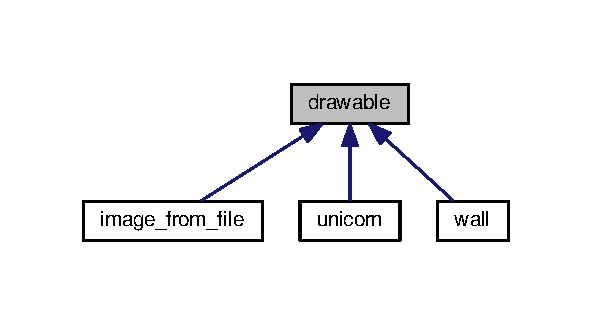
\includegraphics[width=350pt]{classdrawable__inherit__graph}
\end{center}
\end{figure}
\subsection*{Public Member Functions}
\begin{DoxyCompactItemize}
\item 
\hyperlink{classdrawable_a4e7881285581530d21b5c9fd59879b30}{drawable} (const sf\+::\+Vector2f \&position, const sf\+::\+Vector2f \&size, std\+::string name)
\begin{DoxyCompactList}\small\item\em constructor for a drawable \end{DoxyCompactList}\item 
virtual void \hyperlink{classdrawable_a4e49e2c1121704c83ce24c5f48dd910f}{draw} (sf\+::\+Render\+Window \&window)=0
\begin{DoxyCompactList}\small\item\em virtual draw function for a drawable \end{DoxyCompactList}\item 
virtual void \hyperlink{classdrawable_ad0d3930c045cc6776aa2c3965be32491}{move} (sf\+::\+Vector2f delta)
\begin{DoxyCompactList}\small\item\em Move function for a drawable. \end{DoxyCompactList}\item 
virtual void \hyperlink{classdrawable_ac39691470b7874f5dec59efe649d3981}{jump} ()
\begin{DoxyCompactList}\small\item\em virtual draw function for a drawable \end{DoxyCompactList}\item 
virtual sf\+::\+Float\+Rect \hyperlink{classdrawable_ae013ac0be47538be9ce885d6642daf73}{get\+Global\+Bounds} ()=0
\begin{DoxyCompactList}\small\item\em virtual get\+Global\+Bounds function \end{DoxyCompactList}\item 
virtual void \hyperlink{classdrawable_a715df01a318331e5611a2b0ad30109ff}{run\+\_\+actions} (object\+\_\+ptr object)
\begin{DoxyCompactList}\small\item\em check and execute actions \end{DoxyCompactList}\item 
virtual bool \hyperlink{classdrawable_a0d3278e4e888fc8289468e8893dd8329}{within} (float x, float a, float b)
\begin{DoxyCompactList}\small\item\em check x between a and b \end{DoxyCompactList}\item 
virtual bool \hyperlink{classdrawable_ab5c0e1af885f214bc9ef0da47cdb5ac9}{within\+\_\+range} (float x, float y, float a, float b)
\begin{DoxyCompactList}\small\item\em check all pixels between x and y \end{DoxyCompactList}\item 
virtual void \hyperlink{classdrawable_af0ddd3660d258629598dc76b31d1cc49}{collapse} (object\+\_\+ptr object, collisions \&the\+\_\+collisions)
\begin{DoxyCompactList}\small\item\em check for collision with object \end{DoxyCompactList}\item 
virtual sf\+::\+Vector2f \hyperlink{classdrawable_a6a31ea381be2964d0115b782a66d3414}{get\+\_\+position} ()
\begin{DoxyCompactList}\small\item\em Get the position. \end{DoxyCompactList}\item 
virtual sf\+::\+Vector2f \hyperlink{classdrawable_a58cb3ab0406d40e9cea3aefac1e4bf05}{get\+\_\+size} ()
\begin{DoxyCompactList}\small\item\em get size \end{DoxyCompactList}\item 
virtual \hyperlink{structcollision}{collision} \hyperlink{classdrawable_abbc6e0089d502ba48c3fcb9c96e3966e}{check\+\_\+for\+\_\+collisions} (char c)
\begin{DoxyCompactList}\small\item\em check for collisions \end{DoxyCompactList}\item 
virtual std\+::string \hyperlink{classdrawable_a2ed0f8bb53f33477f7722efa7bb24583}{object\+\_\+information} ()
\begin{DoxyCompactList}\small\item\em object information as string \end{DoxyCompactList}\item 
virtual std\+::string \hyperlink{classdrawable_add3d8569fe2616ae0ed503b19c92c08e}{string\+\_\+from\+\_\+color} (sf\+::\+Color \&col)
\begin{DoxyCompactList}\small\item\em object information as string \end{DoxyCompactList}\item 
std\+::string \hyperlink{classdrawable_a329e564296d591dc8bd2f6dc5a205213}{get\+\_\+type} ()
\begin{DoxyCompactList}\small\item\em Get the type. \end{DoxyCompactList}\item 
void \hyperlink{classdrawable_aa019787b726542ca470fb817251e7b09}{set\+\_\+type} (std\+::string s)
\begin{DoxyCompactList}\small\item\em Set the type. \end{DoxyCompactList}\item 
void \hyperlink{classdrawable_a34b6b50f342c41f550f09e0465f95f61}{set\+\_\+size} (sf\+::\+Vector2f new\+\_\+size)
\begin{DoxyCompactList}\small\item\em Set the size. \end{DoxyCompactList}\item 
void \hyperlink{classdrawable_a5e40f2621daaca4ac32ef26b8c01b9a6}{set\+\_\+position} (sf\+::\+Vector2f new\+\_\+position)
\begin{DoxyCompactList}\small\item\em Set the position. \end{DoxyCompactList}\end{DoxyCompactItemize}
\subsection*{Protected Attributes}
\begin{DoxyCompactItemize}
\item 
\mbox{\Hypertarget{classdrawable_a34679fa5ae82eee65dfd6b1b9f3c7cb6}\label{classdrawable_a34679fa5ae82eee65dfd6b1b9f3c7cb6}} 
sf\+::\+Vector2f {\bfseries position}
\item 
\mbox{\Hypertarget{classdrawable_aa3900dd7b69b439a3514e6acdb4a17b9}\label{classdrawable_aa3900dd7b69b439a3514e6acdb4a17b9}} 
sf\+::\+Vector2f {\bfseries size}
\item 
\mbox{\Hypertarget{classdrawable_ad5a982912d20a94b0e69de86cc9b53cb}\label{classdrawable_ad5a982912d20a94b0e69de86cc9b53cb}} 
std\+::string {\bfseries type}
\end{DoxyCompactItemize}


\subsection{Detailed Description}
class that is inherited by all objects that are drawable 

class with a position, size and type, that is inherited by all object that can be drawn on the screen. 

\subsection{Constructor \& Destructor Documentation}
\mbox{\Hypertarget{classdrawable_a4e7881285581530d21b5c9fd59879b30}\label{classdrawable_a4e7881285581530d21b5c9fd59879b30}} 
\index{drawable@{drawable}!drawable@{drawable}}
\index{drawable@{drawable}!drawable@{drawable}}
\subsubsection{\texorpdfstring{drawable()}{drawable()}}
{\footnotesize\ttfamily drawable\+::drawable (\begin{DoxyParamCaption}\item[{const sf\+::\+Vector2f \&}]{position,  }\item[{const sf\+::\+Vector2f \&}]{size,  }\item[{std\+::string}]{name }\end{DoxyParamCaption})}



constructor for a drawable 

constructor that initializes position, size and name of drawable


\begin{DoxyParams}[1]{Parameters}
\mbox{\tt in}  & {\em position} & Position of drawable, this is a sf\+::\+Vector2f and const \\
\hline
\mbox{\tt in}  & {\em size} & Tize of drawable, this is a sf\+::\+Vector2f and const \\
\hline
\mbox{\tt in}  & {\em name} & This is the name of the drawable and is an std\+::string \\
\hline
\end{DoxyParams}


\subsection{Member Function Documentation}
\mbox{\Hypertarget{classdrawable_abbc6e0089d502ba48c3fcb9c96e3966e}\label{classdrawable_abbc6e0089d502ba48c3fcb9c96e3966e}} 
\index{drawable@{drawable}!check\+\_\+for\+\_\+collisions@{check\+\_\+for\+\_\+collisions}}
\index{check\+\_\+for\+\_\+collisions@{check\+\_\+for\+\_\+collisions}!drawable@{drawable}}
\subsubsection{\texorpdfstring{check\+\_\+for\+\_\+collisions()}{check\_for\_collisions()}}
{\footnotesize\ttfamily virtual \hyperlink{structcollision}{collision} drawable\+::check\+\_\+for\+\_\+collisions (\begin{DoxyParamCaption}\item[{char}]{c }\end{DoxyParamCaption})\hspace{0.3cm}{\ttfamily [inline]}, {\ttfamily [virtual]}}



check for collisions 

This function returns a collision struct type that is empty. The function needs to be fully implemented in subclasses if they need it.


\begin{DoxyParams}[1]{Parameters}
\mbox{\tt in}  & {\em c} & The collision side that needs to be checked \\
\hline
\end{DoxyParams}


Reimplemented in \hyperlink{classunicorn_a40fe782f273abf46f6121db9aa4bf77a}{unicorn}.

\mbox{\Hypertarget{classdrawable_af0ddd3660d258629598dc76b31d1cc49}\label{classdrawable_af0ddd3660d258629598dc76b31d1cc49}} 
\index{drawable@{drawable}!collapse@{collapse}}
\index{collapse@{collapse}!drawable@{drawable}}
\subsubsection{\texorpdfstring{collapse()}{collapse()}}
{\footnotesize\ttfamily void drawable\+::collapse (\begin{DoxyParamCaption}\item[{object\+\_\+ptr}]{object,  }\item[{collisions \&}]{the\+\_\+collisions }\end{DoxyParamCaption})\hspace{0.3cm}{\ttfamily [virtual]}}



check for collision with object 

This function checks if this object is colliding with another object. The output is put into a vector of collisions.


\begin{DoxyParams}[1]{Parameters}
\mbox{\tt in}  & {\em object} & The other object for the collision check \\
\hline
\mbox{\tt out}  & {\em the\+\_\+collisions} & The vector to put the collision in \\
\hline
\end{DoxyParams}
\mbox{\Hypertarget{classdrawable_a4e49e2c1121704c83ce24c5f48dd910f}\label{classdrawable_a4e49e2c1121704c83ce24c5f48dd910f}} 
\index{drawable@{drawable}!draw@{draw}}
\index{draw@{draw}!drawable@{drawable}}
\subsubsection{\texorpdfstring{draw()}{draw()}}
{\footnotesize\ttfamily virtual void drawable\+::draw (\begin{DoxyParamCaption}\item[{sf\+::\+Render\+Window \&}]{window }\end{DoxyParamCaption})\hspace{0.3cm}{\ttfamily [pure virtual]}}



virtual draw function for a drawable 

virtual function that is defined in the subclasses of drawable


\begin{DoxyParams}[1]{Parameters}
\mbox{\tt in}  & {\em window} & S\+F\+ML window that is used to display the drawable \\
\hline
\end{DoxyParams}


Implemented in \hyperlink{classanimation_a20959b66d1c25007890bb40f0e876570}{animation}, \hyperlink{classbullet_ae999b952538687d45ca2ae54164a5cd8}{bullet}, \hyperlink{classunicorn_a570c34d5669a8d2a61bdc1481e6f9dee}{unicorn}, \hyperlink{classimage__from__file_a26eae6c872ca9033cacc3f6eb2762983}{image\+\_\+from\+\_\+file}, \hyperlink{classmob_a52f5e29b2ac2d87c8c1be7e0ff5ec96b}{mob}, \hyperlink{classbackground_a41736f9a00defad1e84b3a8099c887e2}{background}, and \hyperlink{classwall_aa25b8377e1d9a209fabd2271294f05d0}{wall}.

\mbox{\Hypertarget{classdrawable_a6a31ea381be2964d0115b782a66d3414}\label{classdrawable_a6a31ea381be2964d0115b782a66d3414}} 
\index{drawable@{drawable}!get\+\_\+position@{get\+\_\+position}}
\index{get\+\_\+position@{get\+\_\+position}!drawable@{drawable}}
\subsubsection{\texorpdfstring{get\+\_\+position()}{get\_position()}}
{\footnotesize\ttfamily sf\+::\+Vector2f drawable\+::get\+\_\+position (\begin{DoxyParamCaption}{ }\end{DoxyParamCaption})\hspace{0.3cm}{\ttfamily [virtual]}}



Get the position. 

This function returns the position of the object. \mbox{\Hypertarget{classdrawable_a58cb3ab0406d40e9cea3aefac1e4bf05}\label{classdrawable_a58cb3ab0406d40e9cea3aefac1e4bf05}} 
\index{drawable@{drawable}!get\+\_\+size@{get\+\_\+size}}
\index{get\+\_\+size@{get\+\_\+size}!drawable@{drawable}}
\subsubsection{\texorpdfstring{get\+\_\+size()}{get\_size()}}
{\footnotesize\ttfamily sf\+::\+Vector2f drawable\+::get\+\_\+size (\begin{DoxyParamCaption}{ }\end{DoxyParamCaption})\hspace{0.3cm}{\ttfamily [virtual]}}



get size 

This function returns the size of the object.

\begin{DoxyReturn}{Returns}
The size of the object 
\end{DoxyReturn}
\mbox{\Hypertarget{classdrawable_a329e564296d591dc8bd2f6dc5a205213}\label{classdrawable_a329e564296d591dc8bd2f6dc5a205213}} 
\index{drawable@{drawable}!get\+\_\+type@{get\+\_\+type}}
\index{get\+\_\+type@{get\+\_\+type}!drawable@{drawable}}
\subsubsection{\texorpdfstring{get\+\_\+type()}{get\_type()}}
{\footnotesize\ttfamily std\+::string drawable\+::get\+\_\+type (\begin{DoxyParamCaption}{ }\end{DoxyParamCaption})}



Get the type. 

This function returns the type of the object.

\begin{DoxyReturn}{Returns}
The type of the object 
\end{DoxyReturn}
\mbox{\Hypertarget{classdrawable_ae013ac0be47538be9ce885d6642daf73}\label{classdrawable_ae013ac0be47538be9ce885d6642daf73}} 
\index{drawable@{drawable}!get\+Global\+Bounds@{get\+Global\+Bounds}}
\index{get\+Global\+Bounds@{get\+Global\+Bounds}!drawable@{drawable}}
\subsubsection{\texorpdfstring{get\+Global\+Bounds()}{getGlobalBounds()}}
{\footnotesize\ttfamily virtual sf\+::\+Float\+Rect drawable\+::get\+Global\+Bounds (\begin{DoxyParamCaption}{ }\end{DoxyParamCaption})\hspace{0.3cm}{\ttfamily [pure virtual]}}



virtual get\+Global\+Bounds function 

virtual function that gives \#sf\+::\+Floatrect of perimeter from the drawable 

Implemented in \hyperlink{classanimation_aae3322323bf3dea83723969f364e18e0}{animation}, \hyperlink{classunicorn_a1bac09fc59b04f14f5a093bc4daa04da}{unicorn}, \hyperlink{classbullet_a87bda5887249e8e37c5579180449bd93}{bullet}, \hyperlink{classimage__from__file_a971a591f906fa5c6e85b4e32cfc3d6a0}{image\+\_\+from\+\_\+file}, \hyperlink{classmob_af3859378fad2a5f93a1c4d833ff74d5d}{mob}, \hyperlink{classbackground_ab5f2b627cd58e0d07678f0af01c6bd2d}{background}, and \hyperlink{classwall_a317a464c879cfdf9464bd6f1b62d9101}{wall}.

\mbox{\Hypertarget{classdrawable_ac39691470b7874f5dec59efe649d3981}\label{classdrawable_ac39691470b7874f5dec59efe649d3981}} 
\index{drawable@{drawable}!jump@{jump}}
\index{jump@{jump}!drawable@{drawable}}
\subsubsection{\texorpdfstring{jump()}{jump()}}
{\footnotesize\ttfamily virtual void drawable\+::jump (\begin{DoxyParamCaption}{ }\end{DoxyParamCaption})\hspace{0.3cm}{\ttfamily [inline]}, {\ttfamily [virtual]}}



virtual draw function for a drawable 

Virtual function that changes position of drawable to new location given 

Reimplemented in \hyperlink{classunicorn_a07d5ca4e66632c0e871221a27146805a}{unicorn}.

\mbox{\Hypertarget{classdrawable_ad0d3930c045cc6776aa2c3965be32491}\label{classdrawable_ad0d3930c045cc6776aa2c3965be32491}} 
\index{drawable@{drawable}!move@{move}}
\index{move@{move}!drawable@{drawable}}
\subsubsection{\texorpdfstring{move()}{move()}}
{\footnotesize\ttfamily void drawable\+::move (\begin{DoxyParamCaption}\item[{sf\+::\+Vector2f}]{delta }\end{DoxyParamCaption})\hspace{0.3cm}{\ttfamily [virtual]}}



Move function for a drawable. 

Function that moves the drawable with a certian delta


\begin{DoxyParams}[1]{Parameters}
\mbox{\tt in}  & {\em delta} & The delta with wich to move the object. \\
\hline
\end{DoxyParams}


Reimplemented in \hyperlink{classunicorn_a162f200a68342f7bc0baaf17c8cf3f9f}{unicorn}.

\mbox{\Hypertarget{classdrawable_a2ed0f8bb53f33477f7722efa7bb24583}\label{classdrawable_a2ed0f8bb53f33477f7722efa7bb24583}} 
\index{drawable@{drawable}!object\+\_\+information@{object\+\_\+information}}
\index{object\+\_\+information@{object\+\_\+information}!drawable@{drawable}}
\subsubsection{\texorpdfstring{object\+\_\+information()}{object\_information()}}
{\footnotesize\ttfamily std\+::string drawable\+::object\+\_\+information (\begin{DoxyParamCaption}{ }\end{DoxyParamCaption})\hspace{0.3cm}{\ttfamily [virtual]}}



object information as string 

This function returns al the object information. The information is returned as a string an contains the type and the position.

output example\+: W\+A\+LL (0.\+000000,700.\+000000) \begin{DoxyReturn}{Returns}
The object information 
\end{DoxyReturn}


Reimplemented in \hyperlink{classwall_aab1de4f144f176b134a967ba08747932}{wall}.

\mbox{\Hypertarget{classdrawable_a715df01a318331e5611a2b0ad30109ff}\label{classdrawable_a715df01a318331e5611a2b0ad30109ff}} 
\index{drawable@{drawable}!run\+\_\+actions@{run\+\_\+actions}}
\index{run\+\_\+actions@{run\+\_\+actions}!drawable@{drawable}}
\subsubsection{\texorpdfstring{run\+\_\+actions()}{run\_actions()}}
{\footnotesize\ttfamily virtual void drawable\+::run\+\_\+actions (\begin{DoxyParamCaption}\item[{object\+\_\+ptr}]{object }\end{DoxyParamCaption})\hspace{0.3cm}{\ttfamily [inline]}, {\ttfamily [virtual]}}



check and execute actions 

This function is used to call the operator() on all the actions The run\+\_\+actions function in this superclass is empty. This is for the fact that some subclasses do not have actions. 
\begin{DoxyParams}[1]{Parameters}
\mbox{\tt in}  & {\em object} & The object to use in certain actions \\
\hline
\end{DoxyParams}
\begin{DoxyReturn}{Returns}
sf\+::\+Float\+Rect with the globalbounds 
\end{DoxyReturn}


Reimplemented in \hyperlink{classunicorn_aadb47a9981c46d6add8704074df117df}{unicorn}.

\mbox{\Hypertarget{classdrawable_a5e40f2621daaca4ac32ef26b8c01b9a6}\label{classdrawable_a5e40f2621daaca4ac32ef26b8c01b9a6}} 
\index{drawable@{drawable}!set\+\_\+position@{set\+\_\+position}}
\index{set\+\_\+position@{set\+\_\+position}!drawable@{drawable}}
\subsubsection{\texorpdfstring{set\+\_\+position()}{set\_position()}}
{\footnotesize\ttfamily void drawable\+::set\+\_\+position (\begin{DoxyParamCaption}\item[{sf\+::\+Vector2f}]{new\+\_\+position }\end{DoxyParamCaption})}



Set the position. 

This function sets the position of an object to a new position.


\begin{DoxyParams}[1]{Parameters}
\mbox{\tt in}  & {\em new\+\_\+position} & The new position for the object \\
\hline
\end{DoxyParams}
\mbox{\Hypertarget{classdrawable_a34b6b50f342c41f550f09e0465f95f61}\label{classdrawable_a34b6b50f342c41f550f09e0465f95f61}} 
\index{drawable@{drawable}!set\+\_\+size@{set\+\_\+size}}
\index{set\+\_\+size@{set\+\_\+size}!drawable@{drawable}}
\subsubsection{\texorpdfstring{set\+\_\+size()}{set\_size()}}
{\footnotesize\ttfamily void drawable\+::set\+\_\+size (\begin{DoxyParamCaption}\item[{sf\+::\+Vector2f}]{new\+\_\+size }\end{DoxyParamCaption})}



Set the size. 

This function sets the size of an object to a new size.


\begin{DoxyParams}[1]{Parameters}
\mbox{\tt in}  & {\em new\+\_\+size} & The new size for the object \\
\hline
\end{DoxyParams}
\mbox{\Hypertarget{classdrawable_aa019787b726542ca470fb817251e7b09}\label{classdrawable_aa019787b726542ca470fb817251e7b09}} 
\index{drawable@{drawable}!set\+\_\+type@{set\+\_\+type}}
\index{set\+\_\+type@{set\+\_\+type}!drawable@{drawable}}
\subsubsection{\texorpdfstring{set\+\_\+type()}{set\_type()}}
{\footnotesize\ttfamily void drawable\+::set\+\_\+type (\begin{DoxyParamCaption}\item[{std\+::string}]{s }\end{DoxyParamCaption})}



Set the type. 

This function sets the type of the object to a new type.


\begin{DoxyParams}[1]{Parameters}
\mbox{\tt in}  & {\em s} & The new type for the object \\
\hline
\end{DoxyParams}
\mbox{\Hypertarget{classdrawable_add3d8569fe2616ae0ed503b19c92c08e}\label{classdrawable_add3d8569fe2616ae0ed503b19c92c08e}} 
\index{drawable@{drawable}!string\+\_\+from\+\_\+color@{string\+\_\+from\+\_\+color}}
\index{string\+\_\+from\+\_\+color@{string\+\_\+from\+\_\+color}!drawable@{drawable}}
\subsubsection{\texorpdfstring{string\+\_\+from\+\_\+color()}{string\_from\_color()}}
{\footnotesize\ttfamily std\+::string drawable\+::string\+\_\+from\+\_\+color (\begin{DoxyParamCaption}\item[{sf\+::\+Color \&}]{col }\end{DoxyParamCaption})\hspace{0.3cm}{\ttfamily [virtual]}}



object information as string 

This function returns the color of an object. It requires a color as parameter and converts this to a string.


\begin{DoxyParams}[1]{Parameters}
\mbox{\tt in}  & {\em col} & The color that needs to be converted \\
\hline
\end{DoxyParams}
\begin{DoxyReturn}{Returns}
The color as a string 
\end{DoxyReturn}
\mbox{\Hypertarget{classdrawable_a0d3278e4e888fc8289468e8893dd8329}\label{classdrawable_a0d3278e4e888fc8289468e8893dd8329}} 
\index{drawable@{drawable}!within@{within}}
\index{within@{within}!drawable@{drawable}}
\subsubsection{\texorpdfstring{within()}{within()}}
{\footnotesize\ttfamily bool drawable\+::within (\begin{DoxyParamCaption}\item[{float}]{x,  }\item[{float}]{a,  }\item[{float}]{b }\end{DoxyParamCaption})\hspace{0.3cm}{\ttfamily [virtual]}}



check x between a and b 

This function checks if the x parameter is between the a and b parameters.


\begin{DoxyParams}[1]{Parameters}
\mbox{\tt in}  & {\em x} & The x variable for the check \\
\hline
\mbox{\tt in}  & {\em a} & The a variable for the check \\
\hline
\mbox{\tt in}  & {\em b} & The b variable for the check\\
\hline
\end{DoxyParams}
\begin{DoxyReturn}{Returns}
Returns if x is between a and b 
\end{DoxyReturn}
\mbox{\Hypertarget{classdrawable_ab5c0e1af885f214bc9ef0da47cdb5ac9}\label{classdrawable_ab5c0e1af885f214bc9ef0da47cdb5ac9}} 
\index{drawable@{drawable}!within\+\_\+range@{within\+\_\+range}}
\index{within\+\_\+range@{within\+\_\+range}!drawable@{drawable}}
\subsubsection{\texorpdfstring{within\+\_\+range()}{within\_range()}}
{\footnotesize\ttfamily bool drawable\+::within\+\_\+range (\begin{DoxyParamCaption}\item[{float}]{x,  }\item[{float}]{y,  }\item[{float}]{a,  }\item[{float}]{b }\end{DoxyParamCaption})\hspace{0.3cm}{\ttfamily [virtual]}}



check all pixels between x and y 

This function checks if any pixel between x and y is between a and b.


\begin{DoxyParams}[1]{Parameters}
\mbox{\tt in}  & {\em x} & float The x value of the range of pixels to check \\
\hline
\mbox{\tt in}  & {\em y} & float The y value of the range of pixels to check \\
\hline
\mbox{\tt in}  & {\em a} & float The first value used for checking (a$>$=pixel) \\
\hline
\mbox{\tt in}  & {\em b} & float The second value used for checking (b$<$=pixel)\\
\hline
\end{DoxyParams}
\begin{DoxyReturn}{Returns}
Returns if all pixels between x and y are between a and b 
\end{DoxyReturn}


The documentation for this class was generated from the following files\+:\begin{DoxyCompactItemize}
\item 
\hyperlink{drawable_8hpp}{drawable.\+hpp}\item 
drawable.\+cpp\end{DoxyCompactItemize}

\hypertarget{classend__of__file}{}\section{end\+\_\+of\+\_\+file Class Reference}
\label{classend__of__file}\index{end\+\_\+of\+\_\+file@{end\+\_\+of\+\_\+file}}


End of file error.  




{\ttfamily \#include $<$exceptions.\+hpp$>$}



Inheritance diagram for end\+\_\+of\+\_\+file\+:\nopagebreak
\begin{figure}[H]
\begin{center}
\leavevmode
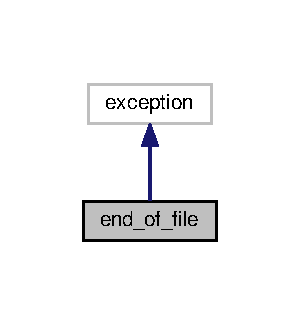
\includegraphics[width=144pt]{classend__of__file__inherit__graph}
\end{center}
\end{figure}


Collaboration diagram for end\+\_\+of\+\_\+file\+:\nopagebreak
\begin{figure}[H]
\begin{center}
\leavevmode
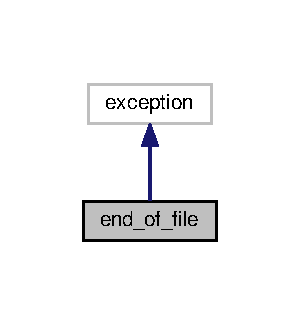
\includegraphics[width=144pt]{classend__of__file__coll__graph}
\end{center}
\end{figure}
\subsection*{Public Member Functions}
\begin{DoxyCompactItemize}
\item 
\hyperlink{classend__of__file_a4e87a15d753f94fad00deee27aa4dc02}{end\+\_\+of\+\_\+file} ()
\begin{DoxyCompactList}\small\item\em Default constructor. \end{DoxyCompactList}\item 
const char $\ast$ \hyperlink{classend__of__file_a32e8c4c2f39a8484c2f39f9a98d5dfb8}{what} () const noexcept override
\begin{DoxyCompactList}\small\item\em Return message. \end{DoxyCompactList}\end{DoxyCompactItemize}


\subsection{Detailed Description}
End of file error. 

This class is used to generate a end of file exception. It inherrits the std\+::exception class so it can be easily caught with an try catch block.

\begin{DoxyDate}{Date}
26-\/1-\/2017 
\end{DoxyDate}


\subsection{Constructor \& Destructor Documentation}
\mbox{\Hypertarget{classend__of__file_a4e87a15d753f94fad00deee27aa4dc02}\label{classend__of__file_a4e87a15d753f94fad00deee27aa4dc02}} 
\index{end\+\_\+of\+\_\+file@{end\+\_\+of\+\_\+file}!end\+\_\+of\+\_\+file@{end\+\_\+of\+\_\+file}}
\index{end\+\_\+of\+\_\+file@{end\+\_\+of\+\_\+file}!end\+\_\+of\+\_\+file@{end\+\_\+of\+\_\+file}}
\subsubsection{\texorpdfstring{end\+\_\+of\+\_\+file()}{end\_of\_file()}}
{\footnotesize\ttfamily end\+\_\+of\+\_\+file\+::end\+\_\+of\+\_\+file (\begin{DoxyParamCaption}{ }\end{DoxyParamCaption})\hspace{0.3cm}{\ttfamily [inline]}}



Default constructor. 

This constructor puts a message into a string and saves that as a private variable. 

\subsection{Member Function Documentation}
\mbox{\Hypertarget{classend__of__file_a32e8c4c2f39a8484c2f39f9a98d5dfb8}\label{classend__of__file_a32e8c4c2f39a8484c2f39f9a98d5dfb8}} 
\index{end\+\_\+of\+\_\+file@{end\+\_\+of\+\_\+file}!what@{what}}
\index{what@{what}!end\+\_\+of\+\_\+file@{end\+\_\+of\+\_\+file}}
\subsubsection{\texorpdfstring{what()}{what()}}
{\footnotesize\ttfamily const char$\ast$ end\+\_\+of\+\_\+file\+::what (\begin{DoxyParamCaption}{ }\end{DoxyParamCaption}) const\hspace{0.3cm}{\ttfamily [inline]}, {\ttfamily [override]}, {\ttfamily [noexcept]}}



Return message. 

This function returns the message so it can be printed. It overrides the what function from the std\+::exception superclass, making it easy to capture.


\begin{DoxyRetVals}{Return values}
{\em const} & char $\ast$ \{The error message as a const char $\ast$\} \\
\hline
\end{DoxyRetVals}


The documentation for this class was generated from the following file\+:\begin{DoxyCompactItemize}
\item 
\hyperlink{exceptions_8hpp}{exceptions.\+hpp}\end{DoxyCompactItemize}

\hypertarget{classfactory}{}\section{factory Class Reference}
\label{classfactory}\index{factory@{factory}}


Factory for reading in levels.  




{\ttfamily \#include $<$factory.\+hpp$>$}

\subsection*{Public Member Functions}
\begin{DoxyCompactItemize}
\item 
\hyperlink{classfactory_af422815046ef8b9e95a4d8cb747fc43f}{factory} (std\+::string filename)
\begin{DoxyCompactList}\small\item\em constructor input file \end{DoxyCompactList}\item 
void \hyperlink{classfactory_a9e164a8fbb65188de99c39d55d7cc384}{change\+\_\+input\+\_\+to} (std\+::string new\+\_\+filename)
\begin{DoxyCompactList}\small\item\em Change the input. \end{DoxyCompactList}\item 
\hyperlink{typedefs_8hpp_aab5add95f06d2ba25dbfed8eb07274fa}{object\+\_\+ptr} \hyperlink{classfactory_a82385866bc910c1b3a3e82d56487dd24}{read\+\_\+line} ()
\begin{DoxyCompactList}\small\item\em Read one line from the filestream. \end{DoxyCompactList}\item 
\hyperlink{typedefs_8hpp_a6c0fdb1dfd0c34dbbdbb5dcd3c608b07}{objects\+\_\+vector} \hyperlink{classfactory_afb2fad4ac9b0f39b1bfc3f3fc8d218b6}{objects\+\_\+from\+\_\+file} ()
\begin{DoxyCompactList}\small\item\em Read multiple objects. \end{DoxyCompactList}\item 
void \hyperlink{classfactory_af17f2a44d75cf8ccf712384341c2fcde}{write\+\_\+information\+\_\+to\+\_\+file} (\hyperlink{typedefs_8hpp_a6c0fdb1dfd0c34dbbdbb5dcd3c608b07}{objects\+\_\+vector} \&objects, std\+::string new\+\_\+filename)
\begin{DoxyCompactList}\small\item\em Write information to file. \end{DoxyCompactList}\item 
sf\+::\+Vector2f \hyperlink{classfactory_a3c3a039b8f76a947267dbe659166550b}{get\+\_\+spawn} ()
\begin{DoxyCompactList}\small\item\em Get spawn location. \end{DoxyCompactList}\item 
sf\+::\+Vector2f \hyperlink{classfactory_af9bb026273b34fc032ca5ac73d457611}{get\+\_\+level\+\_\+size} ()
\begin{DoxyCompactList}\small\item\em Get the level size. \end{DoxyCompactList}\end{DoxyCompactItemize}


\subsection{Detailed Description}
Factory for reading in levels. 

This class is for reading in levels using a factory pattern. It uses smart pointers for making sure that destruction of the created heap objects is done correctly. \begin{DoxyDate}{Date}
26-\/1-\/17 
\end{DoxyDate}


\subsection{Constructor \& Destructor Documentation}
\mbox{\Hypertarget{classfactory_af422815046ef8b9e95a4d8cb747fc43f}\label{classfactory_af422815046ef8b9e95a4d8cb747fc43f}} 
\index{factory@{factory}!factory@{factory}}
\index{factory@{factory}!factory@{factory}}
\subsubsection{\texorpdfstring{factory()}{factory()}}
{\footnotesize\ttfamily factory\+::factory (\begin{DoxyParamCaption}\item[{std\+::string}]{filename }\end{DoxyParamCaption})}



constructor input file 

This constructor receives an input file to read the level out of. That level can be changed later to read in new levels using the \hyperlink{classfactory_a9e164a8fbb65188de99c39d55d7cc384}{factory\+::change\+\_\+input\+\_\+to()} function. The received file name gets the .properties extension and a filestream object is created. 
\begin{DoxyParams}[1]{Parameters}
\mbox{\tt in}  & {\em filename} & The file to open as a filestream object \\
\hline
\end{DoxyParams}
\begin{DoxyNote}{Note}
The filename automatically gets the extension .properties 
\end{DoxyNote}


\subsection{Member Function Documentation}
\mbox{\Hypertarget{classfactory_a9e164a8fbb65188de99c39d55d7cc384}\label{classfactory_a9e164a8fbb65188de99c39d55d7cc384}} 
\index{factory@{factory}!change\+\_\+input\+\_\+to@{change\+\_\+input\+\_\+to}}
\index{change\+\_\+input\+\_\+to@{change\+\_\+input\+\_\+to}!factory@{factory}}
\subsubsection{\texorpdfstring{change\+\_\+input\+\_\+to()}{change\_input\_to()}}
{\footnotesize\ttfamily void factory\+::change\+\_\+input\+\_\+to (\begin{DoxyParamCaption}\item[{std\+::string}]{new\+\_\+filename }\end{DoxyParamCaption})}



Change the input. 

This function changes the input to a new specified file. It also closes the old file if it is open. 
\begin{DoxyParams}[1]{Parameters}
\mbox{\tt in}  & {\em new\+\_\+filename} & The name of the new file to open \\
\hline
\end{DoxyParams}
\mbox{\Hypertarget{classfactory_af9bb026273b34fc032ca5ac73d457611}\label{classfactory_af9bb026273b34fc032ca5ac73d457611}} 
\index{factory@{factory}!get\+\_\+level\+\_\+size@{get\+\_\+level\+\_\+size}}
\index{get\+\_\+level\+\_\+size@{get\+\_\+level\+\_\+size}!factory@{factory}}
\subsubsection{\texorpdfstring{get\+\_\+level\+\_\+size()}{get\_level\_size()}}
{\footnotesize\ttfamily sf\+::\+Vector2f factory\+::get\+\_\+level\+\_\+size (\begin{DoxyParamCaption}{ }\end{DoxyParamCaption})}



Get the level size. 

This function returns the level size.

\begin{DoxyReturn}{Returns}
The level size 
\end{DoxyReturn}
\mbox{\Hypertarget{classfactory_a3c3a039b8f76a947267dbe659166550b}\label{classfactory_a3c3a039b8f76a947267dbe659166550b}} 
\index{factory@{factory}!get\+\_\+spawn@{get\+\_\+spawn}}
\index{get\+\_\+spawn@{get\+\_\+spawn}!factory@{factory}}
\subsubsection{\texorpdfstring{get\+\_\+spawn()}{get\_spawn()}}
{\footnotesize\ttfamily sf\+::\+Vector2f factory\+::get\+\_\+spawn (\begin{DoxyParamCaption}{ }\end{DoxyParamCaption})}



Get spawn location. 

This function returns the spawn location for the level

\begin{DoxyReturn}{Returns}
The spawn location 
\end{DoxyReturn}
\mbox{\Hypertarget{classfactory_afb2fad4ac9b0f39b1bfc3f3fc8d218b6}\label{classfactory_afb2fad4ac9b0f39b1bfc3f3fc8d218b6}} 
\index{factory@{factory}!objects\+\_\+from\+\_\+file@{objects\+\_\+from\+\_\+file}}
\index{objects\+\_\+from\+\_\+file@{objects\+\_\+from\+\_\+file}!factory@{factory}}
\subsubsection{\texorpdfstring{objects\+\_\+from\+\_\+file()}{objects\_from\_file()}}
{\footnotesize\ttfamily \hyperlink{typedefs_8hpp_a6c0fdb1dfd0c34dbbdbb5dcd3c608b07}{objects\+\_\+vector} factory\+::objects\+\_\+from\+\_\+file (\begin{DoxyParamCaption}{ }\end{DoxyParamCaption})}



Read multiple objects. 

This function continuesly calls the \hyperlink{classfactory_a82385866bc910c1b3a3e82d56487dd24}{factory\+::read\+\_\+line()} function and fills an \hyperlink{typedefs_8hpp_a6c0fdb1dfd0c34dbbdbb5dcd3c608b07}{objects\+\_\+vector} with \hyperlink{classdrawable}{drawable} objects. This filled vector is returned. The errors returned by the \hyperlink{classfactory_a82385866bc910c1b3a3e82d56487dd24}{read\+\_\+line()} function are also handled in this function. \begin{DoxyReturn}{Returns}
The vector with the created objects 
\end{DoxyReturn}
\mbox{\Hypertarget{classfactory_a82385866bc910c1b3a3e82d56487dd24}\label{classfactory_a82385866bc910c1b3a3e82d56487dd24}} 
\index{factory@{factory}!read\+\_\+line@{read\+\_\+line}}
\index{read\+\_\+line@{read\+\_\+line}!factory@{factory}}
\subsubsection{\texorpdfstring{read\+\_\+line()}{read\_line()}}
{\footnotesize\ttfamily \hyperlink{typedefs_8hpp_aab5add95f06d2ba25dbfed8eb07274fa}{object\+\_\+ptr} factory\+::read\+\_\+line (\begin{DoxyParamCaption}{ }\end{DoxyParamCaption})}



Read one line from the filestream. 

This function reads one line from the filestream opened in the constructor. It returns a smart pointer to the object it received or a number of different kind of errors. The errors that can be thrown back are\+: \hyperlink{classunknown__type}{unknown\+\_\+type}, \char`\"{}\+L\+E\+V\+E\+L\+\_\+\+S\+I\+Z\+E\char`\"{} and \char`\"{}\+S\+P\+A\+W\+N\char`\"{}. The level\+\_\+size and spawn errors are for when the code receives the spawn and level size from the file it is reading. \begin{DoxyReturn}{Returns}
The shared pointer to the drawable object 
\end{DoxyReturn}
\mbox{\Hypertarget{classfactory_af17f2a44d75cf8ccf712384341c2fcde}\label{classfactory_af17f2a44d75cf8ccf712384341c2fcde}} 
\index{factory@{factory}!write\+\_\+information\+\_\+to\+\_\+file@{write\+\_\+information\+\_\+to\+\_\+file}}
\index{write\+\_\+information\+\_\+to\+\_\+file@{write\+\_\+information\+\_\+to\+\_\+file}!factory@{factory}}
\subsubsection{\texorpdfstring{write\+\_\+information\+\_\+to\+\_\+file()}{write\_information\_to\_file()}}
{\footnotesize\ttfamily void factory\+::write\+\_\+information\+\_\+to\+\_\+file (\begin{DoxyParamCaption}\item[{\hyperlink{typedefs_8hpp_a6c0fdb1dfd0c34dbbdbb5dcd3c608b07}{objects\+\_\+vector} \&}]{objects,  }\item[{std\+::string}]{new\+\_\+filename }\end{DoxyParamCaption})}



Write information to file. 

This function writes all the information on the objects to an output file that is specified in the parameters. It first closes any input files and then opens the output file. After this it outputs the spawn location and level size calls the \hyperlink{classdrawable_a2ed0f8bb53f33477f7722efa7bb24583}{drawable\+::object\+\_\+information()} function on every item in the vector. You end up with an output like this\+: S\+P\+A\+WN (1030,1500) L\+E\+V\+E\+L\+\_\+\+S\+I\+ZE (4000,3350) W\+A\+LL (1020.\+000000,2000.\+000000) (100.\+000000,20.\+000000) green grass.\+png 
\begin{DoxyParams}[1]{Parameters}
\mbox{\tt in}  & {\em objects} & The \hyperlink{typedefs_8hpp_a6c0fdb1dfd0c34dbbdbb5dcd3c608b07}{objects\+\_\+vector} that contains all the objects we want to write to the file \\
\hline
\mbox{\tt in}  & {\em new\+\_\+filename} & The file to write the information to \\
\hline
\end{DoxyParams}


The documentation for this class was generated from the following files\+:\begin{DoxyCompactItemize}
\item 
\hyperlink{factory_8hpp}{factory.\+hpp}\item 
factory.\+cpp\end{DoxyCompactItemize}

\hypertarget{classfile__management}{}\section{file\+\_\+management Class Reference}
\label{classfile__management}\index{file\+\_\+management@{file\+\_\+management}}


file manager for the save-\/files  




{\ttfamily \#include $<$management.\+hpp$>$}



Collaboration diagram for file\+\_\+management\+:
\nopagebreak
\begin{figure}[H]
\begin{center}
\leavevmode
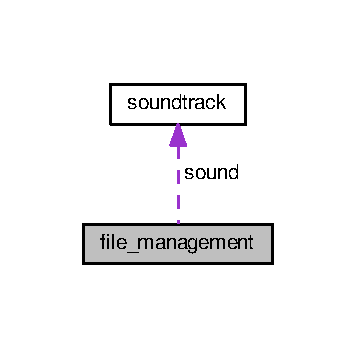
\includegraphics[width=171pt]{classfile__management__coll__graph}
\end{center}
\end{figure}
\subsection*{Public Member Functions}
\begin{DoxyCompactItemize}
\item 
\hyperlink{classfile__management_a1c9de5c140a469a9d0f82970929f4a83}{file\+\_\+management} (std\+::string pathfile, sf\+::\+Render\+Window \&window, \hyperlink{classsoundtrack}{soundtrack} \&sound)
\begin{DoxyCompactList}\small\item\em constructor to initialize pathfile \end{DoxyCompactList}\item 
void \hyperlink{classfile__management_a090d9aba4dd5a795428ccbfe8d4037e6}{set\+\_\+input} (std\+::string new\+\_\+filename)
\begin{DoxyCompactList}\small\item\em function that changes input that is used for information \end{DoxyCompactList}\item 
std\+::string \hyperlink{classfile__management_a6c3f90ce958156adea878510097d64ef}{get\+\_\+files} ()
\begin{DoxyCompactList}\small\item\em function that loads input from file \end{DoxyCompactList}\item 
std\+::string \hyperlink{classfile__management_a58233800263bf74ae074a9a46f4a7bd0}{get\+\_\+level\+\_\+file} (std\+::string save\+\_\+file)
\begin{DoxyCompactList}\small\item\em function that returns path to level given save-\/file \end{DoxyCompactList}\item 
\hyperlink{classmenu}{menu} \hyperlink{classfile__management_a97eda13bca5dbe703663bf81f83a77a0}{make\+\_\+save\+\_\+file\+\_\+menu} (sf\+::\+Render\+Window \&window)
\begin{DoxyCompactList}\small\item\em function that rerturns menu-\/object \end{DoxyCompactList}\item 
std\+::string \hyperlink{classfile__management_a75689c420580c71f0621dfbcc4c2a06f}{next\+\_\+level} ()
\begin{DoxyCompactList}\small\item\em function that returns next level path \end{DoxyCompactList}\item 
void \hyperlink{classfile__management_a291475384add5bdb8002127c71c568ac}{set\+\_\+counter} (int value)
\begin{DoxyCompactList}\small\item\em function that sets counter \end{DoxyCompactList}\item 
int \& \hyperlink{classfile__management_ae6291547fab57a5b861c52e970175854}{get\+\_\+counter} ()
\begin{DoxyCompactList}\small\item\em getter for the counter of the level \end{DoxyCompactList}\item 
std\+::string \hyperlink{classfile__management_a92ece2d05964c828dcb9bf6c59043327}{get\+\_\+save\+\_\+file} (int menu\+\_\+index)
\begin{DoxyCompactList}\small\item\em function that returns path to save-\/file given menu item pushed \end{DoxyCompactList}\item 
void \hyperlink{classfile__management_a79e6ae7cec63aa959d7d0730d6ffa5a3}{save\+\_\+game} ()
\begin{DoxyCompactList}\small\item\em function that saves game \end{DoxyCompactList}\end{DoxyCompactItemize}
\subsection*{Private Attributes}
\begin{DoxyCompactItemize}
\item 
\mbox{\Hypertarget{classfile__management_ae918c94705d91703f7305439f34e07f8}\label{classfile__management_ae918c94705d91703f7305439f34e07f8}} 
sf\+::\+Render\+Window \& {\bfseries window}
\item 
\mbox{\Hypertarget{classfile__management_ae7074fbc5ae0481d0d94c33c4e5890e4}\label{classfile__management_ae7074fbc5ae0481d0d94c33c4e5890e4}} 
\hyperlink{classsoundtrack}{soundtrack} \& {\bfseries sound}
\item 
\mbox{\Hypertarget{classfile__management_aa5b855928609e6725e9912d4d5113455}\label{classfile__management_aa5b855928609e6725e9912d4d5113455}} 
std\+::ifstream {\bfseries input}
\item 
\mbox{\Hypertarget{classfile__management_af8152191fda966b0f308a33f530278da}\label{classfile__management_af8152191fda966b0f308a33f530278da}} 
std\+::ofstream {\bfseries output}
\item 
\mbox{\Hypertarget{classfile__management_a503b8f617941c7bcce5fd6d1898fceae}\label{classfile__management_a503b8f617941c7bcce5fd6d1898fceae}} 
std\+::string {\bfseries save\+\_\+file\+\_\+1}
\item 
\mbox{\Hypertarget{classfile__management_aa5040a08dff914b113025893ef56ad45}\label{classfile__management_aa5040a08dff914b113025893ef56ad45}} 
std\+::string {\bfseries save\+\_\+file\+\_\+2}
\item 
\mbox{\Hypertarget{classfile__management_a93097112df7cf7b9783004c8c8ce19eb}\label{classfile__management_a93097112df7cf7b9783004c8c8ce19eb}} 
int {\bfseries counter}
\item 
\mbox{\Hypertarget{classfile__management_a3089e02713d9608fa342ea5673a88845}\label{classfile__management_a3089e02713d9608fa342ea5673a88845}} 
int {\bfseries current\+\_\+save\+\_\+file} = 0
\item 
\mbox{\Hypertarget{classfile__management_ab08321ef015c6e8843b4632b3ae9c463}\label{classfile__management_ab08321ef015c6e8843b4632b3ae9c463}} 
std\+::string {\bfseries standard\+\_\+path} = \char`\"{}levels/\char`\"{}
\end{DoxyCompactItemize}


\subsection{Detailed Description}
file manager for the save-\/files 

This class reads the save-\/files and gives back the path to the level in the save file. This function can also be used for loading the path to the level after the one your currently playing

\begin{DoxyDate}{Date}
30-\/1-\/17 
\end{DoxyDate}


\subsection{Constructor \& Destructor Documentation}
\mbox{\Hypertarget{classfile__management_a1c9de5c140a469a9d0f82970929f4a83}\label{classfile__management_a1c9de5c140a469a9d0f82970929f4a83}} 
\index{file\+\_\+management@{file\+\_\+management}!file\+\_\+management@{file\+\_\+management}}
\index{file\+\_\+management@{file\+\_\+management}!file\+\_\+management@{file\+\_\+management}}
\subsubsection{\texorpdfstring{file\+\_\+management()}{file\_management()}}
{\footnotesize\ttfamily file\+\_\+management\+::file\+\_\+management (\begin{DoxyParamCaption}\item[{std\+::string}]{pathfile,  }\item[{sf\+::\+Render\+Window \&}]{window,  }\item[{\hyperlink{classsoundtrack}{soundtrack} \&}]{sound }\end{DoxyParamCaption})}



constructor to initialize pathfile 

This constructor sets input equal to the pathfile given.


\begin{DoxyParams}[1]{Parameters}
\mbox{\tt in}  & {\em pathfile} & The pathfile that contains all save\+\_\+file paths \\
\hline
\end{DoxyParams}


\subsection{Member Function Documentation}
\mbox{\Hypertarget{classfile__management_ae6291547fab57a5b861c52e970175854}\label{classfile__management_ae6291547fab57a5b861c52e970175854}} 
\index{file\+\_\+management@{file\+\_\+management}!get\+\_\+counter@{get\+\_\+counter}}
\index{get\+\_\+counter@{get\+\_\+counter}!file\+\_\+management@{file\+\_\+management}}
\subsubsection{\texorpdfstring{get\+\_\+counter()}{get\_counter()}}
{\footnotesize\ttfamily int \& file\+\_\+management\+::get\+\_\+counter (\begin{DoxyParamCaption}{ }\end{DoxyParamCaption})}



getter for the counter of the level 

returns the counter in reference so it makes the counter lookable every moment \mbox{\Hypertarget{classfile__management_a6c3f90ce958156adea878510097d64ef}\label{classfile__management_a6c3f90ce958156adea878510097d64ef}} 
\index{file\+\_\+management@{file\+\_\+management}!get\+\_\+files@{get\+\_\+files}}
\index{get\+\_\+files@{get\+\_\+files}!file\+\_\+management@{file\+\_\+management}}
\subsubsection{\texorpdfstring{get\+\_\+files()}{get\_files()}}
{\footnotesize\ttfamily std\+::string file\+\_\+management\+::get\+\_\+files (\begin{DoxyParamCaption}{ }\end{DoxyParamCaption})}



function that loads input from file 

This function loads input from file that is used as input file. returns one line at the time.

\begin{DoxyReturn}{Returns}
std\+::string that is the content of the line of the file 
\end{DoxyReturn}
\mbox{\Hypertarget{classfile__management_a58233800263bf74ae074a9a46f4a7bd0}\label{classfile__management_a58233800263bf74ae074a9a46f4a7bd0}} 
\index{file\+\_\+management@{file\+\_\+management}!get\+\_\+level\+\_\+file@{get\+\_\+level\+\_\+file}}
\index{get\+\_\+level\+\_\+file@{get\+\_\+level\+\_\+file}!file\+\_\+management@{file\+\_\+management}}
\subsubsection{\texorpdfstring{get\+\_\+level\+\_\+file()}{get\_level\_file()}}
{\footnotesize\ttfamily std\+::string file\+\_\+management\+::get\+\_\+level\+\_\+file (\begin{DoxyParamCaption}\item[{std\+::string}]{save\+\_\+file }\end{DoxyParamCaption})}



function that returns path to level given save-\/file 

This function gets the path of the level currently in the save-\/file, it also reads this string and determines which level the file is. Then sets the counter to that level.


\begin{DoxyParams}[1]{Parameters}
\mbox{\tt in}  & {\em save\+\_\+file} & path to file that contains path to level\\
\hline
\end{DoxyParams}
\begin{DoxyReturn}{Returns}
std\+::string that contains path to level in save\+\_\+file 
\end{DoxyReturn}
\mbox{\Hypertarget{classfile__management_a92ece2d05964c828dcb9bf6c59043327}\label{classfile__management_a92ece2d05964c828dcb9bf6c59043327}} 
\index{file\+\_\+management@{file\+\_\+management}!get\+\_\+save\+\_\+file@{get\+\_\+save\+\_\+file}}
\index{get\+\_\+save\+\_\+file@{get\+\_\+save\+\_\+file}!file\+\_\+management@{file\+\_\+management}}
\subsubsection{\texorpdfstring{get\+\_\+save\+\_\+file()}{get\_save\_file()}}
{\footnotesize\ttfamily std\+::string file\+\_\+management\+::get\+\_\+save\+\_\+file (\begin{DoxyParamCaption}\item[{int}]{menu\+\_\+index }\end{DoxyParamCaption})}



function that returns path to save-\/file given menu item pushed 

This function returns the path to the save-\/file of the given menu\+\_\+index, for example\+: If the first menu item (in this game \char`\"{}\+S\+A\+V\+E 1\char`\"{}) is pressed. The menu\+\_\+index is entered (1) and the return is the path to save file 1


\begin{DoxyParams}[1]{Parameters}
\mbox{\tt in}  & {\em menu\+\_\+index} & index of the menu button pressed.\\
\hline
\end{DoxyParams}
\begin{DoxyReturn}{Returns}
std\+::string that contains path to save-\/file 
\end{DoxyReturn}
\mbox{\Hypertarget{classfile__management_a97eda13bca5dbe703663bf81f83a77a0}\label{classfile__management_a97eda13bca5dbe703663bf81f83a77a0}} 
\index{file\+\_\+management@{file\+\_\+management}!make\+\_\+save\+\_\+file\+\_\+menu@{make\+\_\+save\+\_\+file\+\_\+menu}}
\index{make\+\_\+save\+\_\+file\+\_\+menu@{make\+\_\+save\+\_\+file\+\_\+menu}!file\+\_\+management@{file\+\_\+management}}
\subsubsection{\texorpdfstring{make\+\_\+save\+\_\+file\+\_\+menu()}{make\_save\_file\_menu()}}
{\footnotesize\ttfamily \hyperlink{classmenu}{menu} file\+\_\+management\+::make\+\_\+save\+\_\+file\+\_\+menu (\begin{DoxyParamCaption}\item[{sf\+::\+Render\+Window \&}]{window }\end{DoxyParamCaption})}



function that rerturns menu-\/object 

This function makes a menu containing the save-\/files. The size of the menu depends on the amount of save-\/files. This function reads all save\+\_\+files (it also saves them as a private variable) and determines how many menu items it has to make. It returns the created menu.


\begin{DoxyParams}[1]{Parameters}
\mbox{\tt in}  & {\em window} & sf\+::\+Render\+Window from S\+F\+ML that is used to display the menu on\\
\hline
\end{DoxyParams}
\begin{DoxyReturn}{Returns}
menu-\/object that is used in \hyperlink{classmenu__management}{menu\+\_\+management} 
\end{DoxyReturn}
\mbox{\Hypertarget{classfile__management_a75689c420580c71f0621dfbcc4c2a06f}\label{classfile__management_a75689c420580c71f0621dfbcc4c2a06f}} 
\index{file\+\_\+management@{file\+\_\+management}!next\+\_\+level@{next\+\_\+level}}
\index{next\+\_\+level@{next\+\_\+level}!file\+\_\+management@{file\+\_\+management}}
\subsubsection{\texorpdfstring{next\+\_\+level()}{next\_level()}}
{\footnotesize\ttfamily std\+::string file\+\_\+management\+::next\+\_\+level (\begin{DoxyParamCaption}{ }\end{DoxyParamCaption})}



function that returns next level path 

This function return string ( that can be fabricated by standard\+\_\+path and the counter) that is used as a path to the next level.

\begin{DoxyReturn}{Returns}
std\+::string that contains path to next level 
\end{DoxyReturn}
\mbox{\Hypertarget{classfile__management_a79e6ae7cec63aa959d7d0730d6ffa5a3}\label{classfile__management_a79e6ae7cec63aa959d7d0730d6ffa5a3}} 
\index{file\+\_\+management@{file\+\_\+management}!save\+\_\+game@{save\+\_\+game}}
\index{save\+\_\+game@{save\+\_\+game}!file\+\_\+management@{file\+\_\+management}}
\subsubsection{\texorpdfstring{save\+\_\+game()}{save\_game()}}
{\footnotesize\ttfamily void file\+\_\+management\+::save\+\_\+game (\begin{DoxyParamCaption}{ }\end{DoxyParamCaption})}



function that saves game 

This function saves your current level path in a save-\/file. Which save file is used to save the path in depends on the save-\/file clicked by the user in the beginning. If you click \char`\"{}new game\char`\"{} the save-\/file is most of the time save-\/file-\/1 only when save-\/file-\/2 is empty it is chosen to write in. \mbox{\Hypertarget{classfile__management_a291475384add5bdb8002127c71c568ac}\label{classfile__management_a291475384add5bdb8002127c71c568ac}} 
\index{file\+\_\+management@{file\+\_\+management}!set\+\_\+counter@{set\+\_\+counter}}
\index{set\+\_\+counter@{set\+\_\+counter}!file\+\_\+management@{file\+\_\+management}}
\subsubsection{\texorpdfstring{set\+\_\+counter()}{set\_counter()}}
{\footnotesize\ttfamily void file\+\_\+management\+::set\+\_\+counter (\begin{DoxyParamCaption}\item[{int}]{value }\end{DoxyParamCaption})}



function that sets counter 

This function sets counter to given value.


\begin{DoxyParams}[1]{Parameters}
\mbox{\tt in}  & {\em value} & integer you want to set value to \\
\hline
\end{DoxyParams}
\mbox{\Hypertarget{classfile__management_a090d9aba4dd5a795428ccbfe8d4037e6}\label{classfile__management_a090d9aba4dd5a795428ccbfe8d4037e6}} 
\index{file\+\_\+management@{file\+\_\+management}!set\+\_\+input@{set\+\_\+input}}
\index{set\+\_\+input@{set\+\_\+input}!file\+\_\+management@{file\+\_\+management}}
\subsubsection{\texorpdfstring{set\+\_\+input()}{set\_input()}}
{\footnotesize\ttfamily void file\+\_\+management\+::set\+\_\+input (\begin{DoxyParamCaption}\item[{std\+::string}]{new\+\_\+filename }\end{DoxyParamCaption})}



function that changes input that is used for information 

This function is used to change the std\+::ifstream to the given file in the parameter


\begin{DoxyParams}[1]{Parameters}
\mbox{\tt in}  & {\em new\+\_\+filename} & Filepath you want to use as input file \\
\hline
\end{DoxyParams}


The documentation for this class was generated from the following files\+:\begin{DoxyCompactItemize}
\item 
\hyperlink{management_8hpp}{management.\+hpp}\item 
management.\+cpp\end{DoxyCompactItemize}

\hypertarget{classfont__load__error}{}\section{font\+\_\+load\+\_\+error Class Reference}
\label{classfont__load__error}\index{font\+\_\+load\+\_\+error@{font\+\_\+load\+\_\+error}}


Can not load font.  




{\ttfamily \#include $<$exceptions.\+hpp$>$}



Inheritance diagram for font\+\_\+load\+\_\+error\+:\nopagebreak
\begin{figure}[H]
\begin{center}
\leavevmode
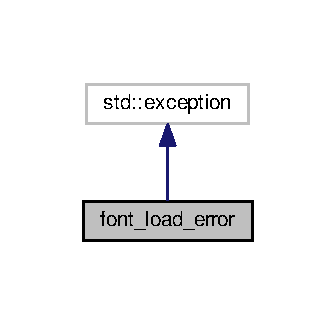
\includegraphics[width=161pt]{classfont__load__error__inherit__graph}
\end{center}
\end{figure}


Collaboration diagram for font\+\_\+load\+\_\+error\+:\nopagebreak
\begin{figure}[H]
\begin{center}
\leavevmode
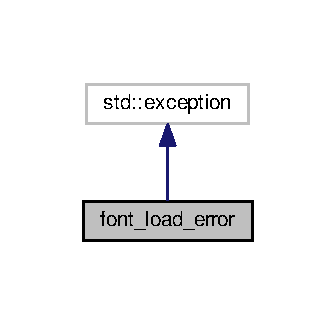
\includegraphics[width=161pt]{classfont__load__error__coll__graph}
\end{center}
\end{figure}
\subsection*{Public Member Functions}
\begin{DoxyCompactItemize}
\item 
\hyperlink{classfont__load__error_ae7d125fc4bd751d97556cb343a6c6fc4}{font\+\_\+load\+\_\+error} (const std\+::string font)
\begin{DoxyCompactList}\small\item\em Constructor. \end{DoxyCompactList}\item 
const char $\ast$ \hyperlink{classfont__load__error_a17c3014c5953ab5863585e4cbf8865c3}{what} () const noexcept override
\begin{DoxyCompactList}\small\item\em Return message. \end{DoxyCompactList}\end{DoxyCompactItemize}
\subsection*{Private Attributes}
\begin{DoxyCompactItemize}
\item 
\mbox{\Hypertarget{classfont__load__error_a7e5ccc82a1685b59ac6ecaadbc956397}\label{classfont__load__error_a7e5ccc82a1685b59ac6ecaadbc956397}} 
std\+::string {\bfseries msg}
\end{DoxyCompactItemize}


\subsection{Detailed Description}
Can not load font. 

This class is used to generate a ufont load exception. It inherrits the std\+::exception class so it can be easily caught with an try catch block.

\begin{DoxyDate}{Date}
31-\/1-\/2017 
\end{DoxyDate}


\subsection{Constructor \& Destructor Documentation}
\mbox{\Hypertarget{classfont__load__error_ae7d125fc4bd751d97556cb343a6c6fc4}\label{classfont__load__error_ae7d125fc4bd751d97556cb343a6c6fc4}} 
\index{font\+\_\+load\+\_\+error@{font\+\_\+load\+\_\+error}!font\+\_\+load\+\_\+error@{font\+\_\+load\+\_\+error}}
\index{font\+\_\+load\+\_\+error@{font\+\_\+load\+\_\+error}!font\+\_\+load\+\_\+error@{font\+\_\+load\+\_\+error}}
\subsubsection{\texorpdfstring{font\+\_\+load\+\_\+error()}{font\_load\_error()}}
{\footnotesize\ttfamily font\+\_\+load\+\_\+error\+::font\+\_\+load\+\_\+error (\begin{DoxyParamCaption}\item[{const std\+::string}]{font }\end{DoxyParamCaption})\hspace{0.3cm}{\ttfamily [inline]}}



Constructor. 

This constructor puts a message into a string and saves that as a private variable. The font name is also added to the string.


\begin{DoxyParams}[1]{Parameters}
\mbox{\tt in}  & {\em font} & The name of the font \\
\hline
\end{DoxyParams}


\subsection{Member Function Documentation}
\mbox{\Hypertarget{classfont__load__error_a17c3014c5953ab5863585e4cbf8865c3}\label{classfont__load__error_a17c3014c5953ab5863585e4cbf8865c3}} 
\index{font\+\_\+load\+\_\+error@{font\+\_\+load\+\_\+error}!what@{what}}
\index{what@{what}!font\+\_\+load\+\_\+error@{font\+\_\+load\+\_\+error}}
\subsubsection{\texorpdfstring{what()}{what()}}
{\footnotesize\ttfamily const char$\ast$ font\+\_\+load\+\_\+error\+::what (\begin{DoxyParamCaption}{ }\end{DoxyParamCaption}) const\hspace{0.3cm}{\ttfamily [inline]}, {\ttfamily [override]}, {\ttfamily [noexcept]}}



Return message. 

This function returns the message so it can be printed. It overrides the what function from the std\+::exception superclass, making it easy to capture.


\begin{DoxyRetVals}{Return values}
{\em const} & char $\ast$ \{The error message as a const char $\ast$\} \\
\hline
\end{DoxyRetVals}


The documentation for this class was generated from the following file\+:\begin{DoxyCompactItemize}
\item 
\hyperlink{exceptions_8hpp}{exceptions.\+hpp}\end{DoxyCompactItemize}

\hypertarget{classimage__from__file}{}\section{image\+\_\+from\+\_\+file Class Reference}
\label{classimage__from__file}\index{image\+\_\+from\+\_\+file@{image\+\_\+from\+\_\+file}}


create sprite on screen  




{\ttfamily \#include $<$image.\+hpp$>$}



Inheritance diagram for image\+\_\+from\+\_\+file\+:\nopagebreak
\begin{figure}[H]
\begin{center}
\leavevmode
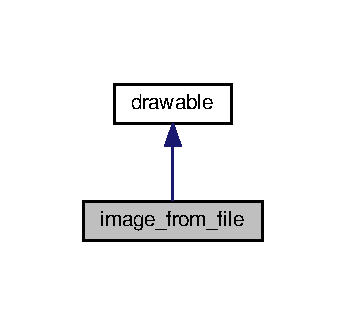
\includegraphics[width=166pt]{classimage__from__file__inherit__graph}
\end{center}
\end{figure}


Collaboration diagram for image\+\_\+from\+\_\+file\+:\nopagebreak
\begin{figure}[H]
\begin{center}
\leavevmode
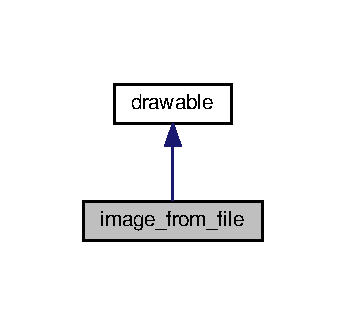
\includegraphics[width=166pt]{classimage__from__file__coll__graph}
\end{center}
\end{figure}
\subsection*{Public Member Functions}
\begin{DoxyCompactItemize}
\item 
\hyperlink{classimage__from__file_a08fd7ad55a2eb520242e31ff3cdf2663}{image\+\_\+from\+\_\+file} (sf\+::\+Vector2f position, std\+::string image\+\_\+name)
\begin{DoxyCompactList}\small\item\em constructor \end{DoxyCompactList}\item 
void \hyperlink{classimage__from__file_a26eae6c872ca9033cacc3f6eb2762983}{draw} (sf\+::\+Render\+Window \&window) override
\begin{DoxyCompactList}\small\item\em draw object \end{DoxyCompactList}\item 
sf\+::\+Float\+Rect \hyperlink{classimage__from__file_a971a591f906fa5c6e85b4e32cfc3d6a0}{get\+Global\+Bounds} () override
\begin{DoxyCompactList}\small\item\em get objects floatrect \end{DoxyCompactList}\item 
void \hyperlink{classimage__from__file_a868911f8d541af91290fb8dc56435cd2}{set\+\_\+position} (sf\+::\+Vector2f new\+\_\+position)
\begin{DoxyCompactList}\small\item\em set position \end{DoxyCompactList}\item 
void \hyperlink{classimage__from__file_a43b0d6b11bf46827308e4e6cb7aa8579}{set\+\_\+size} (sf\+::\+Vector2f new\+\_\+size)
\begin{DoxyCompactList}\small\item\em set size \end{DoxyCompactList}\item 
void \hyperlink{classimage__from__file_a6561a7e8833e4ca84ba5a31e98802757}{set\+Texture\+Rect} (const sf\+::\+Int\+Rect \&rectangle)
\begin{DoxyCompactList}\small\item\em set the texture rectangle \end{DoxyCompactList}\end{DoxyCompactItemize}
\subsection*{Additional Inherited Members}


\subsection{Detailed Description}
create sprite on screen 

This class creates an sprite with an image as texture. The class inherrits the superclass drawable.

\begin{DoxySeeAlso}{See also}
\hyperlink{classdrawable}{drawable} 

\href{https://www.sfml-dev.org/documentation/2.0/classsf_1_1Sprite.php }{\tt sf\+::\+Sprite} 

\href{https://www.sfml-dev.org/documentation/2.0/classsf_1_1Texture.php}{\tt sf\+::\+Texture} 
\end{DoxySeeAlso}


\subsection{Constructor \& Destructor Documentation}
\index{image\+\_\+from\+\_\+file@{image\+\_\+from\+\_\+file}!image\+\_\+from\+\_\+file@{image\+\_\+from\+\_\+file}}
\index{image\+\_\+from\+\_\+file@{image\+\_\+from\+\_\+file}!image\+\_\+from\+\_\+file@{image\+\_\+from\+\_\+file}}
\subsubsection[{\texorpdfstring{image\+\_\+from\+\_\+file(sf\+::\+Vector2f position, std\+::string image\+\_\+name)}{image_from_file(sf::Vector2f position, std::string image_name)}}]{\setlength{\rightskip}{0pt plus 5cm}image\+\_\+from\+\_\+file\+::image\+\_\+from\+\_\+file (
\begin{DoxyParamCaption}
\item[{sf\+::\+Vector2f}]{position, }
\item[{std\+::string}]{image\+\_\+name}
\end{DoxyParamCaption}
)}\hypertarget{classimage__from__file_a08fd7ad55a2eb520242e31ff3cdf2663}{}\label{classimage__from__file_a08fd7ad55a2eb520242e31ff3cdf2663}


constructor 

The constructor tries to load an image with the image name specified. If it can not load the image it generates an exception that can be caught with an try, catch block.


\begin{DoxyParams}[1]{Parameters}
\mbox{\tt in}  & {\em position} & The objects initial position \\
\hline
\mbox{\tt in}  & {\em image\+\_\+name} & The name of the image that has to be loaded \\
\hline
\end{DoxyParams}
\begin{DoxySeeAlso}{See also}
\hyperlink{classimage__load__error}{image\+\_\+load\+\_\+error} 
\end{DoxySeeAlso}
\begin{DoxyWarning}{Warning}
Make sure you use a Try catch block to capture the exception generated if the image cannot be loaded 
\end{DoxyWarning}


\subsection{Member Function Documentation}
\index{image\+\_\+from\+\_\+file@{image\+\_\+from\+\_\+file}!draw@{draw}}
\index{draw@{draw}!image\+\_\+from\+\_\+file@{image\+\_\+from\+\_\+file}}
\subsubsection[{\texorpdfstring{draw(sf\+::\+Render\+Window \&window) override}{draw(sf::RenderWindow &window) override}}]{\setlength{\rightskip}{0pt plus 5cm}void image\+\_\+from\+\_\+file\+::draw (
\begin{DoxyParamCaption}
\item[{sf\+::\+Render\+Window \&}]{window}
\end{DoxyParamCaption}
)\hspace{0.3cm}{\ttfamily [override]}, {\ttfamily [virtual]}}\hypertarget{classimage__from__file_a26eae6c872ca9033cacc3f6eb2762983}{}\label{classimage__from__file_a26eae6c872ca9033cacc3f6eb2762983}


draw object 

This function is used for calling the draw function on the sfml object created within this class. It also sets the position for before it draws the object. This way if the position changes, it also changes on screen.


\begin{DoxyParams}[1]{Parameters}
\mbox{\tt in,out}  & {\em window} & The render window to draw the object on \\
\hline
\end{DoxyParams}


Implements \hyperlink{classdrawable_a4e49e2c1121704c83ce24c5f48dd910f}{drawable}.

\index{image\+\_\+from\+\_\+file@{image\+\_\+from\+\_\+file}!get\+Global\+Bounds@{get\+Global\+Bounds}}
\index{get\+Global\+Bounds@{get\+Global\+Bounds}!image\+\_\+from\+\_\+file@{image\+\_\+from\+\_\+file}}
\subsubsection[{\texorpdfstring{get\+Global\+Bounds() override}{getGlobalBounds() override}}]{\setlength{\rightskip}{0pt plus 5cm}sf\+::\+Float\+Rect image\+\_\+from\+\_\+file\+::get\+Global\+Bounds (
\begin{DoxyParamCaption}
{}
\end{DoxyParamCaption}
)\hspace{0.3cm}{\ttfamily [override]}, {\ttfamily [virtual]}}\hypertarget{classimage__from__file_a971a591f906fa5c6e85b4e32cfc3d6a0}{}\label{classimage__from__file_a971a591f906fa5c6e85b4e32cfc3d6a0}


get objects floatrect 

This function uses the get\+Global\+Bounds function from te object to get the bounding box of the object. It returns this as a floatrect. This return value can be used to check if the object touches another object.


\begin{DoxyParams}[1]{Parameters}
\mbox{\tt in}  & {\em position} & The objects initial position \\
\hline
\mbox{\tt in}  & {\em image\+\_\+name} & The name of the image that has to be loaded \\
\hline
\end{DoxyParams}

\begin{DoxyRetVals}{Return values}
{\em sf\+::\+Float\+Rect} & \{The bounding box of the sprite object created in this class\} \\
\hline
\end{DoxyRetVals}


Implements \hyperlink{classdrawable_ae013ac0be47538be9ce885d6642daf73}{drawable}.

\index{image\+\_\+from\+\_\+file@{image\+\_\+from\+\_\+file}!set\+\_\+position@{set\+\_\+position}}
\index{set\+\_\+position@{set\+\_\+position}!image\+\_\+from\+\_\+file@{image\+\_\+from\+\_\+file}}
\subsubsection[{\texorpdfstring{set\+\_\+position(sf\+::\+Vector2f new\+\_\+position)}{set_position(sf::Vector2f new_position)}}]{\setlength{\rightskip}{0pt plus 5cm}void image\+\_\+from\+\_\+file\+::set\+\_\+position (
\begin{DoxyParamCaption}
\item[{sf\+::\+Vector2f}]{new\+\_\+position}
\end{DoxyParamCaption}
)}\hypertarget{classimage__from__file_a868911f8d541af91290fb8dc56435cd2}{}\label{classimage__from__file_a868911f8d541af91290fb8dc56435cd2}


set position 

This function sets the position of the object to a new value.


\begin{DoxyParams}[1]{Parameters}
\mbox{\tt in}  & {\em new\+\_\+position} & sf\+::\+Vector2f The position we want to move the object to \\
\hline
\end{DoxyParams}
\begin{DoxySeeAlso}{See also}
\href{https://www.sfml-dev.org/documentation/2.0/classsf_1_1Vector2.php }{\tt sf\+::\+Vector2f} 
\end{DoxySeeAlso}
\index{image\+\_\+from\+\_\+file@{image\+\_\+from\+\_\+file}!set\+\_\+size@{set\+\_\+size}}
\index{set\+\_\+size@{set\+\_\+size}!image\+\_\+from\+\_\+file@{image\+\_\+from\+\_\+file}}
\subsubsection[{\texorpdfstring{set\+\_\+size(sf\+::\+Vector2f new\+\_\+size)}{set_size(sf::Vector2f new_size)}}]{\setlength{\rightskip}{0pt plus 5cm}void image\+\_\+from\+\_\+file\+::set\+\_\+size (
\begin{DoxyParamCaption}
\item[{sf\+::\+Vector2f}]{new\+\_\+size}
\end{DoxyParamCaption}
)}\hypertarget{classimage__from__file_a43b0d6b11bf46827308e4e6cb7aa8579}{}\label{classimage__from__file_a43b0d6b11bf46827308e4e6cb7aa8579}


set size 

This function sets the size of the object.


\begin{DoxyParams}[1]{Parameters}
\mbox{\tt in}  & {\em new\+\_\+size} & sf\+::\+Vector2f The size we want to set the object to \\
\hline
\end{DoxyParams}
\begin{DoxySeeAlso}{See also}
\href{https://www.sfml-dev.org/documentation/2.0/classsf_1_1Vector2.php }{\tt sf\+::\+Vector2f} 
\end{DoxySeeAlso}
\index{image\+\_\+from\+\_\+file@{image\+\_\+from\+\_\+file}!set\+Texture\+Rect@{set\+Texture\+Rect}}
\index{set\+Texture\+Rect@{set\+Texture\+Rect}!image\+\_\+from\+\_\+file@{image\+\_\+from\+\_\+file}}
\subsubsection[{\texorpdfstring{set\+Texture\+Rect(const sf\+::\+Int\+Rect \&rectangle)}{setTextureRect(const sf::IntRect &rectangle)}}]{\setlength{\rightskip}{0pt plus 5cm}void image\+\_\+from\+\_\+file\+::set\+Texture\+Rect (
\begin{DoxyParamCaption}
\item[{const sf\+::\+Int\+Rect \&}]{rectangle}
\end{DoxyParamCaption}
)}\hypertarget{classimage__from__file_a6561a7e8833e4ca84ba5a31e98802757}{}\label{classimage__from__file_a6561a7e8833e4ca84ba5a31e98802757}


set the texture rectangle 

This function can be used to turn the object around while keeping the same upper left corner as the position of the object.


\begin{DoxyParams}[1]{Parameters}
\mbox{\tt in}  & {\em rectangle} & const sf\+::\+Int\+Rect\& The rectangle box to turn around \\
\hline
\end{DoxyParams}
\begin{DoxySeeAlso}{See also}
\href{https://www.sfml-dev.org/documentation/2.0/classsf_1_1Sprite.php#a3fefec419a4e6a90c0fd54c793d82ec2 }{\tt sf\+::\+Sprite\+::set\+Texture\+Rect sf\+::\+Int\+Rect} 
\end{DoxySeeAlso}


The documentation for this class was generated from the following files\+:\begin{DoxyCompactItemize}
\item 
\hyperlink{image_8hpp}{image.\+hpp}\item 
image.\+cpp\end{DoxyCompactItemize}

\hypertarget{classimage__load__error}{}\section{image\+\_\+load\+\_\+error Class Reference}
\label{classimage__load__error}\index{image\+\_\+load\+\_\+error@{image\+\_\+load\+\_\+error}}


image load error  




{\ttfamily \#include $<$exceptions.\+hpp$>$}



Inheritance diagram for image\+\_\+load\+\_\+error\+:\nopagebreak
\begin{figure}[H]
\begin{center}
\leavevmode
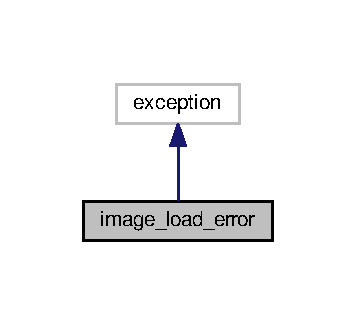
\includegraphics[width=171pt]{classimage__load__error__inherit__graph}
\end{center}
\end{figure}


Collaboration diagram for image\+\_\+load\+\_\+error\+:\nopagebreak
\begin{figure}[H]
\begin{center}
\leavevmode
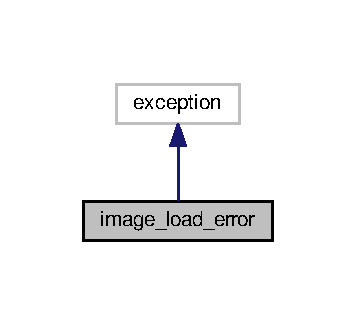
\includegraphics[width=171pt]{classimage__load__error__coll__graph}
\end{center}
\end{figure}
\subsection*{Public Member Functions}
\begin{DoxyCompactItemize}
\item 
\hyperlink{classimage__load__error_a39665f8755ddd18f61bd837300805cd1}{image\+\_\+load\+\_\+error} (const std\+::string \&image\+\_\+name)
\begin{DoxyCompactList}\small\item\em Constructor. \end{DoxyCompactList}\item 
const char $\ast$ \hyperlink{classimage__load__error_ab73fa8f110ff313005a7bb0ed66fd880}{what} () const noexcept override
\begin{DoxyCompactList}\small\item\em Return message. \end{DoxyCompactList}\end{DoxyCompactItemize}
\subsection*{Private Attributes}
\begin{DoxyCompactItemize}
\item 
std\+::string \hyperlink{classimage__load__error_a250134697d7e52db38453039ad59c7df}{msg}
\end{DoxyCompactItemize}


\subsection{Detailed Description}
image load error 

This class is used to generate a image load error exception. It inherrits the std\+::exception class so it can be easily caught with an try catch block.

\begin{DoxyDate}{Date}
19-\/1-\/2017 
\end{DoxyDate}


\subsection{Constructor \& Destructor Documentation}
\mbox{\Hypertarget{classimage__load__error_a39665f8755ddd18f61bd837300805cd1}\label{classimage__load__error_a39665f8755ddd18f61bd837300805cd1}} 
\index{image\+\_\+load\+\_\+error@{image\+\_\+load\+\_\+error}!image\+\_\+load\+\_\+error@{image\+\_\+load\+\_\+error}}
\index{image\+\_\+load\+\_\+error@{image\+\_\+load\+\_\+error}!image\+\_\+load\+\_\+error@{image\+\_\+load\+\_\+error}}
\subsubsection{\texorpdfstring{image\+\_\+load\+\_\+error()}{image\_load\_error()}}
{\footnotesize\ttfamily image\+\_\+load\+\_\+error\+::image\+\_\+load\+\_\+error (\begin{DoxyParamCaption}\item[{const std\+::string \&}]{image\+\_\+name }\end{DoxyParamCaption})\hspace{0.3cm}{\ttfamily [inline]}}



Constructor. 

This constructor puts a message into a string and saves that as a private variable. The image name is also added to the string.


\begin{DoxyParams}[1]{Parameters}
\mbox{\tt in}  & {\em image\+\_\+name} & The name of the image \\
\hline
\end{DoxyParams}


\subsection{Member Function Documentation}
\mbox{\Hypertarget{classimage__load__error_ab73fa8f110ff313005a7bb0ed66fd880}\label{classimage__load__error_ab73fa8f110ff313005a7bb0ed66fd880}} 
\index{image\+\_\+load\+\_\+error@{image\+\_\+load\+\_\+error}!what@{what}}
\index{what@{what}!image\+\_\+load\+\_\+error@{image\+\_\+load\+\_\+error}}
\subsubsection{\texorpdfstring{what()}{what()}}
{\footnotesize\ttfamily const char$\ast$ image\+\_\+load\+\_\+error\+::what (\begin{DoxyParamCaption}{ }\end{DoxyParamCaption}) const\hspace{0.3cm}{\ttfamily [inline]}, {\ttfamily [override]}, {\ttfamily [noexcept]}}



Return message. 

This function returns the message so it can be printed. It overrides the what function from the std\+::exception superclass, making it easy to capture.


\begin{DoxyRetVals}{Return values}
{\em const} & char $\ast$ \{The error message as a const char $\ast$\} \\
\hline
\end{DoxyRetVals}


\subsection{Member Data Documentation}
\mbox{\Hypertarget{classimage__load__error_a250134697d7e52db38453039ad59c7df}\label{classimage__load__error_a250134697d7e52db38453039ad59c7df}} 
\index{image\+\_\+load\+\_\+error@{image\+\_\+load\+\_\+error}!msg@{msg}}
\index{msg@{msg}!image\+\_\+load\+\_\+error@{image\+\_\+load\+\_\+error}}
\subsubsection{\texorpdfstring{msg}{msg}}
{\footnotesize\ttfamily std\+::string image\+\_\+load\+\_\+error\+::msg\hspace{0.3cm}{\ttfamily [private]}}



The documentation for this class was generated from the following file\+:\begin{DoxyCompactItemize}
\item 
\hyperlink{exceptions_8hpp}{exceptions.\+hpp}\end{DoxyCompactItemize}

\hypertarget{classinvalid__position}{}\section{invalid\+\_\+position Class Reference}
\label{classinvalid__position}\index{invalid\+\_\+position@{invalid\+\_\+position}}


Invalid position exception.  




{\ttfamily \#include \char`\"{}exceptions.\+hpp\char`\"{}}



Inheritance diagram for invalid\+\_\+position\+:\nopagebreak
\begin{figure}[H]
\begin{center}
\leavevmode
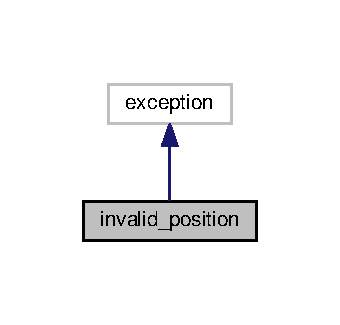
\includegraphics[width=163pt]{classinvalid__position__inherit__graph}
\end{center}
\end{figure}


Collaboration diagram for invalid\+\_\+position\+:\nopagebreak
\begin{figure}[H]
\begin{center}
\leavevmode
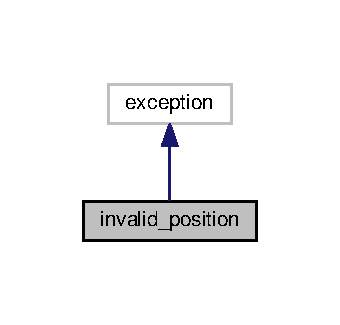
\includegraphics[width=163pt]{classinvalid__position__coll__graph}
\end{center}
\end{figure}
\subsection*{Public Member Functions}
\begin{DoxyCompactItemize}
\item 
\hyperlink{classinvalid__position_a3d39f52e55d28fe6e9b4af02b7c6f278}{invalid\+\_\+position} (const char c)
\begin{DoxyCompactList}\small\item\em Constructor. \end{DoxyCompactList}\item 
\hyperlink{classinvalid__position_aabeae0fae84fada6af68ff83a68c6542}{invalid\+\_\+position} ()
\begin{DoxyCompactList}\small\item\em constructor \end{DoxyCompactList}\item 
const char $\ast$ \hyperlink{classinvalid__position_a7de16130368fed8546deef6713025cfa}{what} () const noexcept override
\begin{DoxyCompactList}\small\item\em Return message. \end{DoxyCompactList}\end{DoxyCompactItemize}
\subsection*{Private Attributes}
\begin{DoxyCompactItemize}
\item 
\mbox{\Hypertarget{classinvalid__position_a53d057adf627ad9d7942a3233bca9028}\label{classinvalid__position_a53d057adf627ad9d7942a3233bca9028}} 
std\+::string {\bfseries msg}
\end{DoxyCompactItemize}


\subsection{Detailed Description}
Invalid position exception. 

This class can be used to generate a exception when a incorrect position has been received using input from a file.

\begin{DoxyDate}{Date}
23-\/1-\/2017 
\end{DoxyDate}


\subsection{Constructor \& Destructor Documentation}
\mbox{\Hypertarget{classinvalid__position_a3d39f52e55d28fe6e9b4af02b7c6f278}\label{classinvalid__position_a3d39f52e55d28fe6e9b4af02b7c6f278}} 
\index{invalid\+\_\+position@{invalid\+\_\+position}!invalid\+\_\+position@{invalid\+\_\+position}}
\index{invalid\+\_\+position@{invalid\+\_\+position}!invalid\+\_\+position@{invalid\+\_\+position}}
\subsubsection{\texorpdfstring{invalid\+\_\+position()}{invalid\_position()}\hspace{0.1cm}{\footnotesize\ttfamily [1/2]}}
{\footnotesize\ttfamily invalid\+\_\+position\+::invalid\+\_\+position (\begin{DoxyParamCaption}\item[{const char}]{c }\end{DoxyParamCaption})\hspace{0.3cm}{\ttfamily [inline]}}



Constructor. 

This constructor puts a message into a string and saves that as a private variable. The character the invalid position was on can also be specified.


\begin{DoxyParams}[1]{Parameters}
\mbox{\tt in}  & {\em c} & The character the error occured on \\
\hline
\end{DoxyParams}
\mbox{\Hypertarget{classinvalid__position_aabeae0fae84fada6af68ff83a68c6542}\label{classinvalid__position_aabeae0fae84fada6af68ff83a68c6542}} 
\index{invalid\+\_\+position@{invalid\+\_\+position}!invalid\+\_\+position@{invalid\+\_\+position}}
\index{invalid\+\_\+position@{invalid\+\_\+position}!invalid\+\_\+position@{invalid\+\_\+position}}
\subsubsection{\texorpdfstring{invalid\+\_\+position()}{invalid\_position()}\hspace{0.1cm}{\footnotesize\ttfamily [2/2]}}
{\footnotesize\ttfamily invalid\+\_\+position\+::invalid\+\_\+position (\begin{DoxyParamCaption}{ }\end{DoxyParamCaption})\hspace{0.3cm}{\ttfamily [inline]}}



constructor 

This constructor puts a message into a string and saves that as a private variable. 

\subsection{Member Function Documentation}
\mbox{\Hypertarget{classinvalid__position_a7de16130368fed8546deef6713025cfa}\label{classinvalid__position_a7de16130368fed8546deef6713025cfa}} 
\index{invalid\+\_\+position@{invalid\+\_\+position}!what@{what}}
\index{what@{what}!invalid\+\_\+position@{invalid\+\_\+position}}
\subsubsection{\texorpdfstring{what()}{what()}}
{\footnotesize\ttfamily const char$\ast$ invalid\+\_\+position\+::what (\begin{DoxyParamCaption}{ }\end{DoxyParamCaption}) const\hspace{0.3cm}{\ttfamily [inline]}, {\ttfamily [override]}, {\ttfamily [noexcept]}}



Return message. 

This function returns the message so it can be printed. It overrides the what function from the std\+::exception superclass, making it easy to capture.


\begin{DoxyRetVals}{Return values}
{\em const} & char $\ast$ \{The error message as a const char $\ast$\} \\
\hline
\end{DoxyRetVals}


The documentation for this class was generated from the following file\+:\begin{DoxyCompactItemize}
\item 
exceptions.\+hpp\end{DoxyCompactItemize}

\hypertarget{classmenu}{}\section{menu Class Reference}
\label{classmenu}\index{menu@{menu}}


Creates a menu with up to 3 buttons.  




{\ttfamily \#include $<$menu.\+hpp$>$}



Collaboration diagram for menu\+:\nopagebreak
\begin{figure}[H]
\begin{center}
\leavevmode
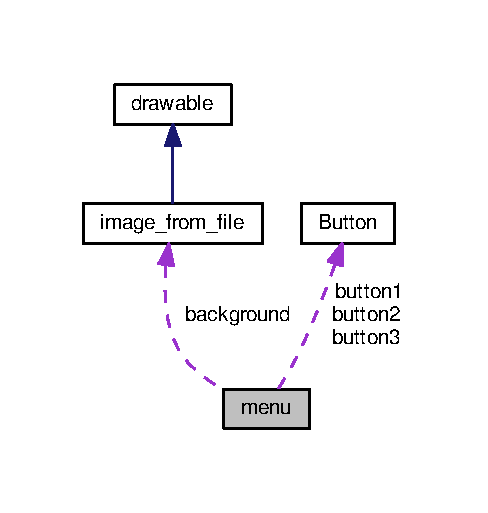
\includegraphics[width=139pt]{classmenu__coll__graph}
\end{center}
\end{figure}
\subsection*{Public Member Functions}
\begin{DoxyCompactItemize}
\item 
\hyperlink{classmenu_a1c6f1319ba2123f9654df695725e83b4}{menu} (sf\+::\+Render\+Window \&\hyperlink{classmenu_a27f2df7cf63febffe1c3c5a5e13ffb8d}{window}, std\+::string \hyperlink{classmenu_af403beeeb7beef5621f0ea806c9f3e6e}{background\+\_\+picture}, bool \hyperlink{classmenu_a044c86b2b6cd959a53f4e92caf34f7a0}{button\+\_\+bool1}, std\+::string \hyperlink{classmenu_a460e3d024e939e6469aede94fd86a64c}{button\+\_\+one\+\_\+text}, bool \hyperlink{classmenu_a043c728ce292a4d87e5e59c9c3db13b9}{button\+\_\+bool2}=0, std\+::string \hyperlink{classmenu_a027f3482fde6a4991ff4036e9e0472bd}{button\+\_\+two\+\_\+text}=\char`\"{}Empty\char`\"{}, bool \hyperlink{classmenu_a469661400ee077af1b949bac629d30c7}{button\+\_\+bool3}=0, std\+::string \hyperlink{classmenu_ac785c6419d139d0181e0487805657e32}{button\+\_\+three\+\_\+text}=\char`\"{}Empty\char`\"{})
\begin{DoxyCompactList}\small\item\em constructor to make a menu \end{DoxyCompactList}\item 
void \hyperlink{classmenu_a8d194b462b1b180086e5b06a2dbfbdff}{build\+\_\+menu} ()
\begin{DoxyCompactList}\small\item\em Function to build and draw the menu. \end{DoxyCompactList}\item 
int \hyperlink{classmenu_a06744d58a2aad693d3637d0485aa7984}{select} (sf\+::\+Vector2i position)
\begin{DoxyCompactList}\small\item\em Function that handles the pushable part of the button. \end{DoxyCompactList}\end{DoxyCompactItemize}
\subsection*{Private Attributes}
\begin{DoxyCompactItemize}
\item 
sf\+::\+Render\+Window \& \hyperlink{classmenu_a27f2df7cf63febffe1c3c5a5e13ffb8d}{window}
\item 
std\+::string \hyperlink{classmenu_af403beeeb7beef5621f0ea806c9f3e6e}{background\+\_\+picture}
\item 
bool \hyperlink{classmenu_a044c86b2b6cd959a53f4e92caf34f7a0}{button\+\_\+bool1}
\item 
bool \hyperlink{classmenu_a043c728ce292a4d87e5e59c9c3db13b9}{button\+\_\+bool2}
\item 
bool \hyperlink{classmenu_a469661400ee077af1b949bac629d30c7}{button\+\_\+bool3}
\item 
std\+::string \hyperlink{classmenu_a460e3d024e939e6469aede94fd86a64c}{button\+\_\+one\+\_\+text}
\item 
std\+::string \hyperlink{classmenu_a027f3482fde6a4991ff4036e9e0472bd}{button\+\_\+two\+\_\+text}
\item 
std\+::string \hyperlink{classmenu_ac785c6419d139d0181e0487805657e32}{button\+\_\+three\+\_\+text}
\item 
\hyperlink{class_button}{Button} \hyperlink{classmenu_a0e51e3f8ef8fd769a42ca9a1ab3ed53e}{button1}
\item 
\hyperlink{class_button}{Button} \hyperlink{classmenu_a3292e41431ba6f6f9a1b08b94206a076}{button2}
\item 
\hyperlink{class_button}{Button} \hyperlink{classmenu_a4f19c398a6009b9d17e197c51ad19a66}{button3}
\end{DoxyCompactItemize}


\subsection{Detailed Description}
Creates a menu with up to 3 buttons. 

This class consists of 3 \hyperlink{class_button}{Button} objects and a \hyperlink{class_background}{Background} object. It creates a menu and also deals with the clickable part of it.

Note\+: We would like to transfer all the math from \hyperlink{class_button}{Button} over here. However, this has low priority .

\begin{DoxyDate}{Date}
27-\/1-\/2017 
\end{DoxyDate}


\subsection{Constructor \& Destructor Documentation}
\mbox{\Hypertarget{classmenu_a1c6f1319ba2123f9654df695725e83b4}\label{classmenu_a1c6f1319ba2123f9654df695725e83b4}} 
\index{menu@{menu}!menu@{menu}}
\index{menu@{menu}!menu@{menu}}
\subsubsection{\texorpdfstring{menu()}{menu()}}
{\footnotesize\ttfamily menu\+::menu (\begin{DoxyParamCaption}\item[{sf\+::\+Render\+Window \&}]{window,  }\item[{std\+::string}]{background\+\_\+picture,  }\item[{bool}]{button\+\_\+bool1,  }\item[{std\+::string}]{button\+\_\+one\+\_\+text,  }\item[{bool}]{button\+\_\+bool2 = {\ttfamily 0},  }\item[{std\+::string}]{button\+\_\+two\+\_\+text = {\ttfamily \char`\"{}Empty\char`\"{}},  }\item[{bool}]{button\+\_\+bool3 = {\ttfamily 0},  }\item[{std\+::string}]{button\+\_\+three\+\_\+text = {\ttfamily \char`\"{}Empty\char`\"{}} }\end{DoxyParamCaption})}



constructor to make a menu 

constructor to make a menu with 1 -\/ 2 or 3 buttons. Also requires a picture for the background. All buttons have default values, so you can specify which buttons you want on the menu.


\begin{DoxyParams}[1]{Parameters}
\mbox{\tt in}  & {\em Window} & Render\+Window \\
\hline
\mbox{\tt in}  & {\em bg\+Picture} & Name and type ( .png ) to load background picture form \\
\hline
\mbox{\tt in}  & {\em button\+Bool1} & Determines if button1 will be drawn \\
\hline
\mbox{\tt in}  & {\em Button\+One\+Text} & Text that will be displayed on button1 \\
\hline
\mbox{\tt in}  & {\em button\+Bool2} & Determines if button2 will be drawn \\
\hline
\mbox{\tt in}  & {\em Button\+Two\+Text} & Text that will be displayed on button2 \\
\hline
\mbox{\tt in}  & {\em button\+Bool3} & Determines if button3 will be drawn \\
\hline
\mbox{\tt in}  & {\em Button\+Three\+Text} & Text that will be displayed on button3 \\
\hline
\end{DoxyParams}


\subsection{Member Function Documentation}
\mbox{\Hypertarget{classmenu_a8d194b462b1b180086e5b06a2dbfbdff}\label{classmenu_a8d194b462b1b180086e5b06a2dbfbdff}} 
\index{menu@{menu}!build\+\_\+menu@{build\+\_\+menu}}
\index{build\+\_\+menu@{build\+\_\+menu}!menu@{menu}}
\subsubsection{\texorpdfstring{build\+\_\+menu()}{build\_menu()}}
{\footnotesize\ttfamily void menu\+::build\+\_\+menu (\begin{DoxyParamCaption}{ }\end{DoxyParamCaption})}



Function to build and draw the menu. 

This function builds the menu, with the buttons that were specified in the constructor. It also handles the drawing of the buttons. \mbox{\Hypertarget{classmenu_a06744d58a2aad693d3637d0485aa7984}\label{classmenu_a06744d58a2aad693d3637d0485aa7984}} 
\index{menu@{menu}!select@{select}}
\index{select@{select}!menu@{menu}}
\subsubsection{\texorpdfstring{select()}{select()}}
{\footnotesize\ttfamily int menu\+::select (\begin{DoxyParamCaption}\item[{sf\+::\+Vector2i}]{position }\end{DoxyParamCaption})}



Function that handles the pushable part of the button. 

This function checks if position is located inside the bounding boxes of the buttons, if yes it will return either a 0 or a 1 or a 2, depending on which button was pushed. This allows different functionality for the three buttons.


\begin{DoxyParams}[1]{Parameters}
\mbox{\tt in}  & {\em position} & The position of the mouse when the left mouse button is pushed \\
\hline
\end{DoxyParams}


\subsection{Member Data Documentation}
\mbox{\Hypertarget{classmenu_af403beeeb7beef5621f0ea806c9f3e6e}\label{classmenu_af403beeeb7beef5621f0ea806c9f3e6e}} 
\index{menu@{menu}!background\+\_\+picture@{background\+\_\+picture}}
\index{background\+\_\+picture@{background\+\_\+picture}!menu@{menu}}
\subsubsection{\texorpdfstring{background\+\_\+picture}{background\_picture}}
{\footnotesize\ttfamily std\+::string menu\+::background\+\_\+picture\hspace{0.3cm}{\ttfamily [private]}}

\mbox{\Hypertarget{classmenu_a0e51e3f8ef8fd769a42ca9a1ab3ed53e}\label{classmenu_a0e51e3f8ef8fd769a42ca9a1ab3ed53e}} 
\index{menu@{menu}!button1@{button1}}
\index{button1@{button1}!menu@{menu}}
\subsubsection{\texorpdfstring{button1}{button1}}
{\footnotesize\ttfamily \hyperlink{class_button}{Button} menu\+::button1\hspace{0.3cm}{\ttfamily [private]}}

\mbox{\Hypertarget{classmenu_a3292e41431ba6f6f9a1b08b94206a076}\label{classmenu_a3292e41431ba6f6f9a1b08b94206a076}} 
\index{menu@{menu}!button2@{button2}}
\index{button2@{button2}!menu@{menu}}
\subsubsection{\texorpdfstring{button2}{button2}}
{\footnotesize\ttfamily \hyperlink{class_button}{Button} menu\+::button2\hspace{0.3cm}{\ttfamily [private]}}

\mbox{\Hypertarget{classmenu_a4f19c398a6009b9d17e197c51ad19a66}\label{classmenu_a4f19c398a6009b9d17e197c51ad19a66}} 
\index{menu@{menu}!button3@{button3}}
\index{button3@{button3}!menu@{menu}}
\subsubsection{\texorpdfstring{button3}{button3}}
{\footnotesize\ttfamily \hyperlink{class_button}{Button} menu\+::button3\hspace{0.3cm}{\ttfamily [private]}}

\mbox{\Hypertarget{classmenu_a044c86b2b6cd959a53f4e92caf34f7a0}\label{classmenu_a044c86b2b6cd959a53f4e92caf34f7a0}} 
\index{menu@{menu}!button\+\_\+bool1@{button\+\_\+bool1}}
\index{button\+\_\+bool1@{button\+\_\+bool1}!menu@{menu}}
\subsubsection{\texorpdfstring{button\+\_\+bool1}{button\_bool1}}
{\footnotesize\ttfamily bool menu\+::button\+\_\+bool1\hspace{0.3cm}{\ttfamily [private]}}

\mbox{\Hypertarget{classmenu_a043c728ce292a4d87e5e59c9c3db13b9}\label{classmenu_a043c728ce292a4d87e5e59c9c3db13b9}} 
\index{menu@{menu}!button\+\_\+bool2@{button\+\_\+bool2}}
\index{button\+\_\+bool2@{button\+\_\+bool2}!menu@{menu}}
\subsubsection{\texorpdfstring{button\+\_\+bool2}{button\_bool2}}
{\footnotesize\ttfamily bool menu\+::button\+\_\+bool2\hspace{0.3cm}{\ttfamily [private]}}

\mbox{\Hypertarget{classmenu_a469661400ee077af1b949bac629d30c7}\label{classmenu_a469661400ee077af1b949bac629d30c7}} 
\index{menu@{menu}!button\+\_\+bool3@{button\+\_\+bool3}}
\index{button\+\_\+bool3@{button\+\_\+bool3}!menu@{menu}}
\subsubsection{\texorpdfstring{button\+\_\+bool3}{button\_bool3}}
{\footnotesize\ttfamily bool menu\+::button\+\_\+bool3\hspace{0.3cm}{\ttfamily [private]}}

\mbox{\Hypertarget{classmenu_a460e3d024e939e6469aede94fd86a64c}\label{classmenu_a460e3d024e939e6469aede94fd86a64c}} 
\index{menu@{menu}!button\+\_\+one\+\_\+text@{button\+\_\+one\+\_\+text}}
\index{button\+\_\+one\+\_\+text@{button\+\_\+one\+\_\+text}!menu@{menu}}
\subsubsection{\texorpdfstring{button\+\_\+one\+\_\+text}{button\_one\_text}}
{\footnotesize\ttfamily std\+::string menu\+::button\+\_\+one\+\_\+text\hspace{0.3cm}{\ttfamily [private]}}

\mbox{\Hypertarget{classmenu_ac785c6419d139d0181e0487805657e32}\label{classmenu_ac785c6419d139d0181e0487805657e32}} 
\index{menu@{menu}!button\+\_\+three\+\_\+text@{button\+\_\+three\+\_\+text}}
\index{button\+\_\+three\+\_\+text@{button\+\_\+three\+\_\+text}!menu@{menu}}
\subsubsection{\texorpdfstring{button\+\_\+three\+\_\+text}{button\_three\_text}}
{\footnotesize\ttfamily std\+::string menu\+::button\+\_\+three\+\_\+text\hspace{0.3cm}{\ttfamily [private]}}

\mbox{\Hypertarget{classmenu_a027f3482fde6a4991ff4036e9e0472bd}\label{classmenu_a027f3482fde6a4991ff4036e9e0472bd}} 
\index{menu@{menu}!button\+\_\+two\+\_\+text@{button\+\_\+two\+\_\+text}}
\index{button\+\_\+two\+\_\+text@{button\+\_\+two\+\_\+text}!menu@{menu}}
\subsubsection{\texorpdfstring{button\+\_\+two\+\_\+text}{button\_two\_text}}
{\footnotesize\ttfamily std\+::string menu\+::button\+\_\+two\+\_\+text\hspace{0.3cm}{\ttfamily [private]}}

\mbox{\Hypertarget{classmenu_a27f2df7cf63febffe1c3c5a5e13ffb8d}\label{classmenu_a27f2df7cf63febffe1c3c5a5e13ffb8d}} 
\index{menu@{menu}!window@{window}}
\index{window@{window}!menu@{menu}}
\subsubsection{\texorpdfstring{window}{window}}
{\footnotesize\ttfamily sf\+::\+Render\+Window\& menu\+::window\hspace{0.3cm}{\ttfamily [private]}}



The documentation for this class was generated from the following files\+:\begin{DoxyCompactItemize}
\item 
\hyperlink{menu_8hpp}{menu.\+hpp}\item 
\hyperlink{menu_8cpp}{menu.\+cpp}\end{DoxyCompactItemize}

\hypertarget{classmenu__management}{}\section{menu\+\_\+management Class Reference}
\label{classmenu__management}\index{menu\+\_\+management@{menu\+\_\+management}}


manager of all menu\textquotesingle{}s in game  




{\ttfamily \#include $<$management.\+hpp$>$}



Collaboration diagram for menu\+\_\+management\+:
\nopagebreak
\begin{figure}[H]
\begin{center}
\leavevmode
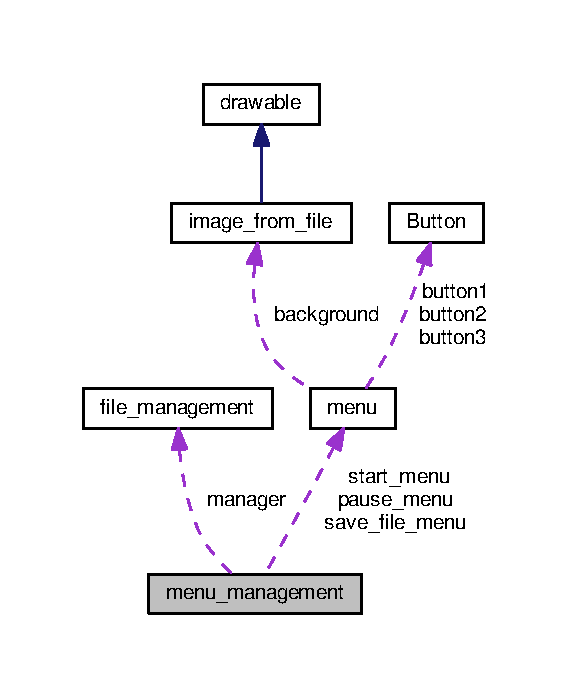
\includegraphics[width=350pt]{classmenu__management__coll__graph}
\end{center}
\end{figure}
\subsection*{Public Member Functions}
\begin{DoxyCompactItemize}
\item 
\hyperlink{classmenu__management_abc65b2b5ef39a07120aed543db8a22b5}{menu\+\_\+management} (sf\+::\+Render\+Window \&window, \hyperlink{classfile__management}{file\+\_\+management} \&manager, \hyperlink{classsoundtrack}{soundtrack} \&sound)
\begin{DoxyCompactList}\small\item\em constructor to initialize window and file manager \end{DoxyCompactList}\item 
int \hyperlink{classmenu__management_aad6e975e03cab2478f3ebec8da7eaf7d}{display\+\_\+start\+\_\+game} ()
\begin{DoxyCompactList}\small\item\em function that displays start\+\_\+menu \end{DoxyCompactList}\item 
void \hyperlink{classmenu__management_ab7aa6674e3428604073af06efe5aa791}{display\+\_\+pause\+\_\+game} ()
\begin{DoxyCompactList}\small\item\em function that displays pause\+\_\+menu \end{DoxyCompactList}\item 
std\+::string \hyperlink{classmenu__management_ac64c1eace3d955be8623a1129597dc54}{display\+\_\+save\+\_\+file\+\_\+menu} ()
\begin{DoxyCompactList}\small\item\em function that displays the save\+\_\+file\+\_\+menu \end{DoxyCompactList}\item 
std\+::string \hyperlink{classmenu__management_a92d22f059d33ccc5c3ae485804fd5fbb}{start\+\_\+game} ()
\begin{DoxyCompactList}\small\item\em function that is used to start the game \end{DoxyCompactList}\end{DoxyCompactItemize}
\subsection*{Private Attributes}
\begin{DoxyCompactItemize}
\item 
\mbox{\Hypertarget{classmenu__management_ab79fa0c3480a52f3cd603c77e8f7008f}\label{classmenu__management_ab79fa0c3480a52f3cd603c77e8f7008f}} 
sf\+::\+Render\+Window \& {\bfseries window}
\item 
\mbox{\Hypertarget{classmenu__management_a0c9bf334940ea0d4576e371e1eaa5c9f}\label{classmenu__management_a0c9bf334940ea0d4576e371e1eaa5c9f}} 
\hyperlink{classfile__management}{file\+\_\+management} \& {\bfseries manager}
\item 
\mbox{\Hypertarget{classmenu__management_aea347d4a93f4e7819dae28b5ba320857}\label{classmenu__management_aea347d4a93f4e7819dae28b5ba320857}} 
\hyperlink{classmenu}{menu} {\bfseries start\+\_\+menu} = \hyperlink{classmenu}{menu}(window,std\+::string\{\char`\"{}forest.\+png\char`\"{}\} , true, \char`\"{}N\+E\+W\+\_\+\+G\+A\+ME\char`\"{}, true, \char`\"{}L\+O\+AD G\+A\+ME\char`\"{}, true, \char`\"{}Q\+U\+IT\char`\"{} )
\item 
\mbox{\Hypertarget{classmenu__management_a125b772090ca2c54c2689b408700eb02}\label{classmenu__management_a125b772090ca2c54c2689b408700eb02}} 
\hyperlink{classmenu}{menu} {\bfseries pause\+\_\+menu} = \hyperlink{classmenu}{menu}(window, std\+::string\{\char`\"{}forest.\+png\char`\"{}\},true, \char`\"{}C\+O\+N\+T\+I\+N\+UE\char`\"{},true ,\char`\"{}Q\+U\+IT\char`\"{})
\item 
\mbox{\Hypertarget{classmenu__management_a1ca190cfc1fcd91354ce00ad5cc1dea6}\label{classmenu__management_a1ca190cfc1fcd91354ce00ad5cc1dea6}} 
\hyperlink{classmenu}{menu} {\bfseries save\+\_\+file\+\_\+menu} = manager.\+make\+\_\+save\+\_\+file\+\_\+menu(window)
\item 
\mbox{\Hypertarget{classmenu__management_a7c05d72347e629a180ff9114295f00d5}\label{classmenu__management_a7c05d72347e629a180ff9114295f00d5}} 
\hyperlink{classsoundtrack}{soundtrack} \& {\bfseries sound}
\end{DoxyCompactItemize}


\subsection{Detailed Description}
manager of all menu\textquotesingle{}s in game 

Manager for the menu\textquotesingle{}s available in the game

\begin{DoxyDate}{Date}
30-\/1-\/17 
\end{DoxyDate}


\subsection{Constructor \& Destructor Documentation}
\mbox{\Hypertarget{classmenu__management_abc65b2b5ef39a07120aed543db8a22b5}\label{classmenu__management_abc65b2b5ef39a07120aed543db8a22b5}} 
\index{menu\+\_\+management@{menu\+\_\+management}!menu\+\_\+management@{menu\+\_\+management}}
\index{menu\+\_\+management@{menu\+\_\+management}!menu\+\_\+management@{menu\+\_\+management}}
\subsubsection{\texorpdfstring{menu\+\_\+management()}{menu\_management()}}
{\footnotesize\ttfamily menu\+\_\+management\+::menu\+\_\+management (\begin{DoxyParamCaption}\item[{sf\+::\+Render\+Window \&}]{window,  }\item[{\hyperlink{classfile__management}{file\+\_\+management} \&}]{manager,  }\item[{\hyperlink{classsoundtrack}{soundtrack} \&}]{sound }\end{DoxyParamCaption})}



constructor to initialize window and file manager 

This constructor initializes the window where the menu\textquotesingle{}s are displayed on. It also initializes the manager for the files


\begin{DoxyParams}[1]{Parameters}
\mbox{\tt in}  & {\em window} & sf\+::\+Render\+Window that is used to display menu\textquotesingle{}s \\
\hline
\mbox{\tt in}  & {\em manager} & filemanagement-\/object that used to give functionality to menu\textquotesingle{}s \\
\hline
\end{DoxyParams}


\subsection{Member Function Documentation}
\mbox{\Hypertarget{classmenu__management_ab7aa6674e3428604073af06efe5aa791}\label{classmenu__management_ab7aa6674e3428604073af06efe5aa791}} 
\index{menu\+\_\+management@{menu\+\_\+management}!display\+\_\+pause\+\_\+game@{display\+\_\+pause\+\_\+game}}
\index{display\+\_\+pause\+\_\+game@{display\+\_\+pause\+\_\+game}!menu\+\_\+management@{menu\+\_\+management}}
\subsubsection{\texorpdfstring{display\+\_\+pause\+\_\+game()}{display\_pause\_game()}}
{\footnotesize\ttfamily void menu\+\_\+management\+::display\+\_\+pause\+\_\+game (\begin{DoxyParamCaption}{ }\end{DoxyParamCaption})}



function that displays pause\+\_\+menu 

This function displays the pause menu

\begin{DoxyNote}{Note}
This function doesn\textquotesingle{}t have a return value, because of a bug this function doesn\textquotesingle{}t have much functionality 
\end{DoxyNote}
\mbox{\Hypertarget{classmenu__management_ac64c1eace3d955be8623a1129597dc54}\label{classmenu__management_ac64c1eace3d955be8623a1129597dc54}} 
\index{menu\+\_\+management@{menu\+\_\+management}!display\+\_\+save\+\_\+file\+\_\+menu@{display\+\_\+save\+\_\+file\+\_\+menu}}
\index{display\+\_\+save\+\_\+file\+\_\+menu@{display\+\_\+save\+\_\+file\+\_\+menu}!menu\+\_\+management@{menu\+\_\+management}}
\subsubsection{\texorpdfstring{display\+\_\+save\+\_\+file\+\_\+menu()}{display\_save\_file\_menu()}}
{\footnotesize\ttfamily std\+::string menu\+\_\+management\+::display\+\_\+save\+\_\+file\+\_\+menu (\begin{DoxyParamCaption}{ }\end{DoxyParamCaption})}



function that displays the save\+\_\+file\+\_\+menu 

F\+This function displays the save\+\_\+file\+\_\+menu. The function return a string from the button pressed. When save-\/file pressed it returns the path to the save-\/file

\begin{DoxyReturn}{Returns}
This function returns a string that is either empty, \char`\"{}\+B\+A\+C\+K\char`\"{} or the path to the save-\/file pressed. 
\end{DoxyReturn}
\mbox{\Hypertarget{classmenu__management_aad6e975e03cab2478f3ebec8da7eaf7d}\label{classmenu__management_aad6e975e03cab2478f3ebec8da7eaf7d}} 
\index{menu\+\_\+management@{menu\+\_\+management}!display\+\_\+start\+\_\+game@{display\+\_\+start\+\_\+game}}
\index{display\+\_\+start\+\_\+game@{display\+\_\+start\+\_\+game}!menu\+\_\+management@{menu\+\_\+management}}
\subsubsection{\texorpdfstring{display\+\_\+start\+\_\+game()}{display\_start\_game()}}
{\footnotesize\ttfamily int menu\+\_\+management\+::display\+\_\+start\+\_\+game (\begin{DoxyParamCaption}{ }\end{DoxyParamCaption})}



function that displays start\+\_\+menu 

This function is used to display the start\+\_\+menu

\begin{DoxyReturn}{Returns}
menu item that is pressed 
\end{DoxyReturn}
\mbox{\Hypertarget{classmenu__management_a92d22f059d33ccc5c3ae485804fd5fbb}\label{classmenu__management_a92d22f059d33ccc5c3ae485804fd5fbb}} 
\index{menu\+\_\+management@{menu\+\_\+management}!start\+\_\+game@{start\+\_\+game}}
\index{start\+\_\+game@{start\+\_\+game}!menu\+\_\+management@{menu\+\_\+management}}
\subsubsection{\texorpdfstring{start\+\_\+game()}{start\_game()}}
{\footnotesize\ttfamily std\+::string menu\+\_\+management\+::start\+\_\+game (\begin{DoxyParamCaption}{ }\end{DoxyParamCaption})}



function that is used to start the game 

This function is used to start the game. By displaying the start screen and determening what level file to use when one is pressed.

\begin{DoxyReturn}{Returns}
path to level selected by player 
\end{DoxyReturn}


The documentation for this class was generated from the following files\+:\begin{DoxyCompactItemize}
\item 
\hyperlink{management_8hpp}{management.\+hpp}\item 
management.\+cpp\end{DoxyCompactItemize}

\hypertarget{classmob}{}\section{mob Class Reference}
\label{classmob}\index{mob@{mob}}


class that makes an enemy to play agianst  




{\ttfamily \#include $<$npc.\+hpp$>$}



Inheritance diagram for mob\+:\nopagebreak
\begin{figure}[H]
\begin{center}
\leavevmode
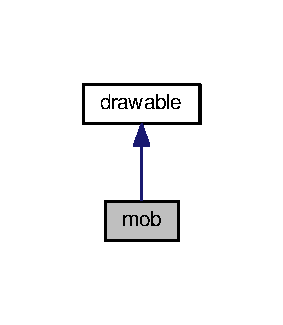
\includegraphics[width=136pt]{classmob__inherit__graph}
\end{center}
\end{figure}


Collaboration diagram for mob\+:\nopagebreak
\begin{figure}[H]
\begin{center}
\leavevmode
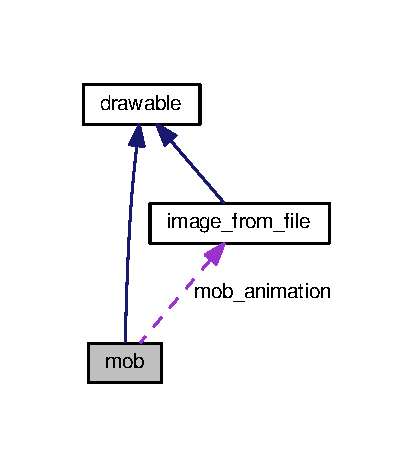
\includegraphics[width=200pt]{classmob__coll__graph}
\end{center}
\end{figure}
\subsection*{Public Member Functions}
\begin{DoxyCompactItemize}
\item 
\hyperlink{classmob_ac524dd40986df00721239b66c552437e}{mob} (sf\+::\+Vector2f position, std\+::string filename)
\begin{DoxyCompactList}\small\item\em constructor to initialize mob \end{DoxyCompactList}\item 
void \hyperlink{classmob_a52f5e29b2ac2d87c8c1be7e0ff5ec96b}{draw} (sf\+::\+Render\+Window \&window) override
\begin{DoxyCompactList}\small\item\em draw function for mob \end{DoxyCompactList}\item 
sf\+::\+Float\+Rect \hyperlink{classmob_af3859378fad2a5f93a1c4d833ff74d5d}{get\+Global\+Bounds} () override
\begin{DoxyCompactList}\small\item\em get function for global bounds \end{DoxyCompactList}\item 
void \hyperlink{classmob_ae892b3ce84f4aa16411b385abb5410c8}{die} ()
\begin{DoxyCompactList}\small\item\em function that sets boolean \end{DoxyCompactList}\item 
void \hyperlink{classmob_a3bce6c06653881f8be86fbc60a2b67cb}{revive} ()
\begin{DoxyCompactList}\small\item\em function that sets boolean \end{DoxyCompactList}\item 
bool \hyperlink{classmob_ab327a1798c02be3f9db7c1d01b17ba02}{get\+\_\+live} ()
\begin{DoxyCompactList}\small\item\em function that returns is\+\_\+alive variable \end{DoxyCompactList}\item 
void \hyperlink{classmob_a6556e84e416fd496450d18dd1d0eb1f2}{set\+\_\+position} (sf\+::\+Vector2f new\+\_\+position)
\begin{DoxyCompactList}\small\item\em set position of the mob \end{DoxyCompactList}\end{DoxyCompactItemize}
\subsection*{Private Attributes}
\begin{DoxyCompactItemize}
\item 
\mbox{\Hypertarget{classmob_a28d29e0a52a7094c995df09dcdcf0d3e}\label{classmob_a28d29e0a52a7094c995df09dcdcf0d3e}} 
\hyperlink{classimage__from__file}{image\+\_\+from\+\_\+file} {\bfseries mob\+\_\+animation}
\item 
\mbox{\Hypertarget{classmob_a395256ca1ea387e4a8867d399e1b0b0b}\label{classmob_a395256ca1ea387e4a8867d399e1b0b0b}} 
bool {\bfseries is\+\_\+alive} = true
\end{DoxyCompactItemize}
\subsection*{Additional Inherited Members}


\subsection{Detailed Description}
class that makes an enemy to play agianst 

This class creates an enemy that the player can shoot this version doesn\textquotesingle{}t include physics for the mob. It also can\textquotesingle{}t fire back.

\begin{DoxyDate}{Date}
26-\/01-\/2017 
\end{DoxyDate}


\subsection{Constructor \& Destructor Documentation}
\mbox{\Hypertarget{classmob_ac524dd40986df00721239b66c552437e}\label{classmob_ac524dd40986df00721239b66c552437e}} 
\index{mob@{mob}!mob@{mob}}
\index{mob@{mob}!mob@{mob}}
\subsubsection{\texorpdfstring{mob()}{mob()}}
{\footnotesize\ttfamily mob\+::mob (\begin{DoxyParamCaption}\item[{sf\+::\+Vector2f}]{position,  }\item[{std\+::string}]{filename }\end{DoxyParamCaption})}



constructor to initialize mob 

This constructor is used to give a position and a name of the file used a image


\begin{DoxyParams}[1]{Parameters}
\mbox{\tt in}  & {\em position} & sf\+::\+Vector2f position where image is placed \\
\hline
\mbox{\tt in}  & {\em filename} & std\+::string that is the filename of the image used \\
\hline
\end{DoxyParams}


\subsection{Member Function Documentation}
\mbox{\Hypertarget{classmob_ae892b3ce84f4aa16411b385abb5410c8}\label{classmob_ae892b3ce84f4aa16411b385abb5410c8}} 
\index{mob@{mob}!die@{die}}
\index{die@{die}!mob@{mob}}
\subsubsection{\texorpdfstring{die()}{die()}}
{\footnotesize\ttfamily void mob\+::die (\begin{DoxyParamCaption}{ }\end{DoxyParamCaption})}



function that sets boolean 

This function sets variable alive to false \mbox{\Hypertarget{classmob_a52f5e29b2ac2d87c8c1be7e0ff5ec96b}\label{classmob_a52f5e29b2ac2d87c8c1be7e0ff5ec96b}} 
\index{mob@{mob}!draw@{draw}}
\index{draw@{draw}!mob@{mob}}
\subsubsection{\texorpdfstring{draw()}{draw()}}
{\footnotesize\ttfamily void mob\+::draw (\begin{DoxyParamCaption}\item[{sf\+::\+Render\+Window \&}]{window }\end{DoxyParamCaption})\hspace{0.3cm}{\ttfamily [override]}, {\ttfamily [virtual]}}



draw function for mob 

This function draws the mob\+\_\+animation. It only draws the mob when it is alive. This can be seen with the \hyperlink{classmob_ab327a1798c02be3f9db7c1d01b17ba02}{mob\+::get\+\_\+live()} function


\begin{DoxyParams}[1]{Parameters}
\mbox{\tt in}  & {\em window} & sf\+::\+Render\+Window that is used to draw picture on \\
\hline
\end{DoxyParams}


Implements \hyperlink{classdrawable_a4e49e2c1121704c83ce24c5f48dd910f}{drawable}.

\mbox{\Hypertarget{classmob_ab327a1798c02be3f9db7c1d01b17ba02}\label{classmob_ab327a1798c02be3f9db7c1d01b17ba02}} 
\index{mob@{mob}!get\+\_\+live@{get\+\_\+live}}
\index{get\+\_\+live@{get\+\_\+live}!mob@{mob}}
\subsubsection{\texorpdfstring{get\+\_\+live()}{get\_live()}}
{\footnotesize\ttfamily bool mob\+::get\+\_\+live (\begin{DoxyParamCaption}{ }\end{DoxyParamCaption})}



function that returns is\+\_\+alive variable 

This function is used to return the current state of the boolean alive

\begin{DoxyReturn}{Returns}
boolean that gives information on if a mob is alive. 
\end{DoxyReturn}
\mbox{\Hypertarget{classmob_af3859378fad2a5f93a1c4d833ff74d5d}\label{classmob_af3859378fad2a5f93a1c4d833ff74d5d}} 
\index{mob@{mob}!get\+Global\+Bounds@{get\+Global\+Bounds}}
\index{get\+Global\+Bounds@{get\+Global\+Bounds}!mob@{mob}}
\subsubsection{\texorpdfstring{get\+Global\+Bounds()}{getGlobalBounds()}}
{\footnotesize\ttfamily sf\+::\+Float\+Rect mob\+::get\+Global\+Bounds (\begin{DoxyParamCaption}{ }\end{DoxyParamCaption})\hspace{0.3cm}{\ttfamily [override]}, {\ttfamily [virtual]}}



get function for global bounds 

This function gets the global bounds of the image in mob. When the mob is not alive gives a empty sf\+::\+Float\+Rect so bullet can\textquotesingle{}t \char`\"{}accidentally\char`\"{} collide with the mob

\begin{DoxyReturn}{Returns}
sf\+::\+Float\+Rect that is empty when mob is not alive 
\end{DoxyReturn}


Implements \hyperlink{classdrawable_ae013ac0be47538be9ce885d6642daf73}{drawable}.

\mbox{\Hypertarget{classmob_a3bce6c06653881f8be86fbc60a2b67cb}\label{classmob_a3bce6c06653881f8be86fbc60a2b67cb}} 
\index{mob@{mob}!revive@{revive}}
\index{revive@{revive}!mob@{mob}}
\subsubsection{\texorpdfstring{revive()}{revive()}}
{\footnotesize\ttfamily void mob\+::revive (\begin{DoxyParamCaption}{ }\end{DoxyParamCaption})}



function that sets boolean 

This function sets variable alive to true \mbox{\Hypertarget{classmob_a6556e84e416fd496450d18dd1d0eb1f2}\label{classmob_a6556e84e416fd496450d18dd1d0eb1f2}} 
\index{mob@{mob}!set\+\_\+position@{set\+\_\+position}}
\index{set\+\_\+position@{set\+\_\+position}!mob@{mob}}
\subsubsection{\texorpdfstring{set\+\_\+position()}{set\_position()}}
{\footnotesize\ttfamily void mob\+::set\+\_\+position (\begin{DoxyParamCaption}\item[{sf\+::\+Vector2f}]{new\+\_\+position }\end{DoxyParamCaption})}



set position of the mob 


\begin{DoxyParams}[1]{Parameters}
\mbox{\tt in}  & {\em new\+\_\+position} & sf\+::\+Vector2f \\
\hline
\end{DoxyParams}


The documentation for this class was generated from the following files\+:\begin{DoxyCompactItemize}
\item 
\hyperlink{npc_8hpp}{npc.\+hpp}\item 
npc.\+cpp\end{DoxyCompactItemize}

\hypertarget{classphysics}{}\section{physics Class Reference}
\label{classphysics}\index{physics@{physics}}


class with physics function  




{\ttfamily \#include $<$physics.\+hpp$>$}

\subsection*{Public Member Functions}
\begin{DoxyCompactItemize}
\item 
void \hyperlink{classphysics_a8b0dff646c304dee3cb5c095d821dc87}{set\+\_\+gravity} (int value)
\begin{DoxyCompactList}\small\item\em set function for the gravity counter. \end{DoxyCompactList}\item 
int \hyperlink{classphysics_a3c4c6084fe0652b0bfd35afa5daa1c1e}{get\+\_\+gravity} ()
\begin{DoxyCompactList}\small\item\em get function for the gravity\+\_\+counter. \end{DoxyCompactList}\item 
float \hyperlink{classphysics_acca1ee2fb8b760b6e4ee61ae7c2ee3da}{falling} ()
\begin{DoxyCompactList}\small\item\em the working function that contains the gavity. \end{DoxyCompactList}\item 
float \hyperlink{classphysics_aaf1c57aa6e35b9c83ccbfdfa8c18468c}{jumping} (int counter)
\begin{DoxyCompactList}\small\item\em the working function for jumping. \end{DoxyCompactList}\end{DoxyCompactItemize}


\subsection{Detailed Description}
class with physics function 

This class containing all forces needed in the game.

\begin{DoxyDate}{Date}
23/01/17 
\end{DoxyDate}


\subsection{Member Function Documentation}
\index{physics@{physics}!falling@{falling}}
\index{falling@{falling}!physics@{physics}}
\subsubsection[{\texorpdfstring{falling()}{falling()}}]{\setlength{\rightskip}{0pt plus 5cm}float physics\+::falling (
\begin{DoxyParamCaption}
{}
\end{DoxyParamCaption}
)}\hypertarget{classphysics_acca1ee2fb8b760b6e4ee61ae7c2ee3da}{}\label{classphysics_acca1ee2fb8b760b6e4ee61ae7c2ee3da}


the working function that contains the gavity. 

float \hyperlink{classphysics_acca1ee2fb8b760b6e4ee61ae7c2ee3da}{falling()}

function that makes falling in the game look natural \index{physics@{physics}!get\+\_\+gravity@{get\+\_\+gravity}}
\index{get\+\_\+gravity@{get\+\_\+gravity}!physics@{physics}}
\subsubsection[{\texorpdfstring{get\+\_\+gravity()}{get_gravity()}}]{\setlength{\rightskip}{0pt plus 5cm}int physics\+::get\+\_\+gravity (
\begin{DoxyParamCaption}
{}
\end{DoxyParamCaption}
)}\hypertarget{classphysics_a3c4c6084fe0652b0bfd35afa5daa1c1e}{}\label{classphysics_a3c4c6084fe0652b0bfd35afa5daa1c1e}


get function for the gravity\+\_\+counter. 

int \hyperlink{classphysics_a3c4c6084fe0652b0bfd35afa5daa1c1e}{get\+\_\+gravity()}

getter for the grafity counter \index{physics@{physics}!jumping@{jumping}}
\index{jumping@{jumping}!physics@{physics}}
\subsubsection[{\texorpdfstring{jumping(int counter)}{jumping(int counter)}}]{\setlength{\rightskip}{0pt plus 5cm}float physics\+::jumping (
\begin{DoxyParamCaption}
\item[{int}]{counter}
\end{DoxyParamCaption}
)}\hypertarget{classphysics_aaf1c57aa6e35b9c83ccbfdfa8c18468c}{}\label{classphysics_aaf1c57aa6e35b9c83ccbfdfa8c18468c}


the working function for jumping. 

float \hyperlink{classphysics_aaf1c57aa6e35b9c83ccbfdfa8c18468c}{jumping(int counter)}

function that makes jumping in the game possible and look natural


\begin{DoxyParams}[1]{Parameters}
\mbox{\tt in}  & {\em counter} & The counter for the jump \\
\hline
\end{DoxyParams}
\index{physics@{physics}!set\+\_\+gravity@{set\+\_\+gravity}}
\index{set\+\_\+gravity@{set\+\_\+gravity}!physics@{physics}}
\subsubsection[{\texorpdfstring{set\+\_\+gravity(int value)}{set_gravity(int value)}}]{\setlength{\rightskip}{0pt plus 5cm}void physics\+::set\+\_\+gravity (
\begin{DoxyParamCaption}
\item[{int}]{value}
\end{DoxyParamCaption}
)}\hypertarget{classphysics_a8b0dff646c304dee3cb5c095d821dc87}{}\label{classphysics_a8b0dff646c304dee3cb5c095d821dc87}


set function for the gravity counter. 

void \hyperlink{classphysics_a8b0dff646c304dee3cb5c095d821dc87}{set\+\_\+gravity(int value)}

setter for the gravity counter 
\begin{DoxyParams}[1]{Parameters}
\mbox{\tt in}  & {\em value} & int where the gravity\+\_\+counter will be set on \\
\hline
\end{DoxyParams}


The documentation for this class was generated from the following files\+:\begin{DoxyCompactItemize}
\item 
physics.\+hpp\item 
physics.\+cpp\end{DoxyCompactItemize}

\hypertarget{classsheet__load__error}{}\section{sheet\+\_\+load\+\_\+error Class Reference}
\label{classsheet__load__error}\index{sheet\+\_\+load\+\_\+error@{sheet\+\_\+load\+\_\+error}}


sheet load error  




{\ttfamily \#include $<$exceptions.\+hpp$>$}



Inheritance diagram for sheet\+\_\+load\+\_\+error\+:\nopagebreak
\begin{figure}[H]
\begin{center}
\leavevmode
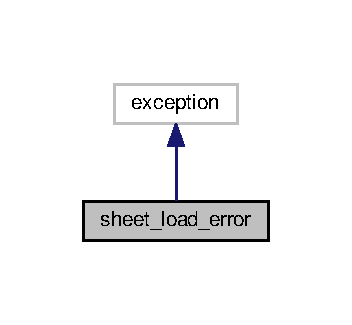
\includegraphics[width=169pt]{classsheet__load__error__inherit__graph}
\end{center}
\end{figure}


Collaboration diagram for sheet\+\_\+load\+\_\+error\+:\nopagebreak
\begin{figure}[H]
\begin{center}
\leavevmode
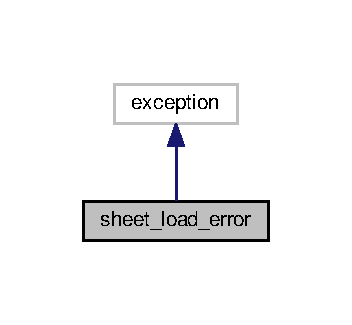
\includegraphics[width=169pt]{classsheet__load__error__coll__graph}
\end{center}
\end{figure}
\subsection*{Public Member Functions}
\begin{DoxyCompactItemize}
\item 
\hyperlink{classsheet__load__error_a80642b59420e3b58c1c5e980cf702c41}{sheet\+\_\+load\+\_\+error} (const std\+::string \&image\+\_\+name)
\begin{DoxyCompactList}\small\item\em constructor \end{DoxyCompactList}\item 
const char $\ast$ \hyperlink{classsheet__load__error_a57dd1a273a0720e58ec0eb667d0c85aa}{what} () const noexcept override
\begin{DoxyCompactList}\small\item\em return message \end{DoxyCompactList}\end{DoxyCompactItemize}


\subsection{Detailed Description}
sheet load error 

This class is used to generate a sheet load error exception. It inherrits the std\+::exception class so it can be easily caught with an try catch block. 

\subsection{Constructor \& Destructor Documentation}
\mbox{\Hypertarget{classsheet__load__error_a80642b59420e3b58c1c5e980cf702c41}\label{classsheet__load__error_a80642b59420e3b58c1c5e980cf702c41}} 
\index{sheet\+\_\+load\+\_\+error@{sheet\+\_\+load\+\_\+error}!sheet\+\_\+load\+\_\+error@{sheet\+\_\+load\+\_\+error}}
\index{sheet\+\_\+load\+\_\+error@{sheet\+\_\+load\+\_\+error}!sheet\+\_\+load\+\_\+error@{sheet\+\_\+load\+\_\+error}}
\subsubsection{\texorpdfstring{sheet\+\_\+load\+\_\+error()}{sheet\_load\_error()}}
{\footnotesize\ttfamily sheet\+\_\+load\+\_\+error\+::sheet\+\_\+load\+\_\+error (\begin{DoxyParamCaption}\item[{const std\+::string \&}]{image\+\_\+name }\end{DoxyParamCaption})\hspace{0.3cm}{\ttfamily [inline]}}



constructor 

This constructor puts a message into a string and saves that as a private variable. The image name is also added to the string.


\begin{DoxyParams}[1]{Parameters}
\mbox{\tt in}  & {\em image\+\_\+name} & The name of the image \\
\hline
\end{DoxyParams}


\subsection{Member Function Documentation}
\mbox{\Hypertarget{classsheet__load__error_a57dd1a273a0720e58ec0eb667d0c85aa}\label{classsheet__load__error_a57dd1a273a0720e58ec0eb667d0c85aa}} 
\index{sheet\+\_\+load\+\_\+error@{sheet\+\_\+load\+\_\+error}!what@{what}}
\index{what@{what}!sheet\+\_\+load\+\_\+error@{sheet\+\_\+load\+\_\+error}}
\subsubsection{\texorpdfstring{what()}{what()}}
{\footnotesize\ttfamily const char$\ast$ sheet\+\_\+load\+\_\+error\+::what (\begin{DoxyParamCaption}{ }\end{DoxyParamCaption}) const\hspace{0.3cm}{\ttfamily [inline]}, {\ttfamily [override]}, {\ttfamily [noexcept]}}



return message 

This function returns the message so it can be printed. It overrides the what function from the std\+::exception superclass, making it easy to capture.


\begin{DoxyRetVals}{Return values}
{\em const} & char $\ast$ \{The error message as a const char $\ast$\} \\
\hline
\end{DoxyRetVals}


The documentation for this class was generated from the following file\+:\begin{DoxyCompactItemize}
\item 
\hyperlink{exceptions_8hpp}{exceptions.\+hpp}\end{DoxyCompactItemize}

\hypertarget{classsoundtrack}{}\section{soundtrack Class Reference}
\label{classsoundtrack}\index{soundtrack@{soundtrack}}


Class that plays either music or sound effects.  




{\ttfamily \#include $<$soundtrack.\+hpp$>$}

\subsection*{Public Member Functions}
\begin{DoxyCompactItemize}
\item 
\hyperlink{classsoundtrack_add31bdeb1a693d541443f1d88586d3b6}{soundtrack} (std\+::string filename)
\begin{DoxyCompactList}\small\item\em constructor for soundtrack class \end{DoxyCompactList}\item 
\mbox{\Hypertarget{classsoundtrack_a9f25fee4c6d5dbc820e2a18b13b43e68}\label{classsoundtrack_a9f25fee4c6d5dbc820e2a18b13b43e68}} 
void {\bfseries stop\+\_\+music} ()
\item 
void \hyperlink{classsoundtrack_a7569a4c0cde86548197756b8e05cf464}{playmusic} ()
\begin{DoxyCompactList}\small\item\em Music player. \end{DoxyCompactList}\item 
void \hyperlink{classsoundtrack_aa18de6469aca15922cfa8a8e8412f76d}{playsound} (std\+::string name)
\begin{DoxyCompactList}\small\item\em Sound player. \end{DoxyCompactList}\item 
\mbox{\Hypertarget{classsoundtrack_a9047bea4f37493cbe81a990bc9d0c4e7}\label{classsoundtrack_a9047bea4f37493cbe81a990bc9d0c4e7}} 
void {\bfseries stop} ()
\item 
\mbox{\Hypertarget{classsoundtrack_a83744518feb748a979a67a56fae997fe}\label{classsoundtrack_a83744518feb748a979a67a56fae997fe}} 
void {\bfseries playsound\+\_\+cutscene} (std\+::string name)
\end{DoxyCompactItemize}


\subsection{Detailed Description}
Class that plays either music or sound effects. 

Class with two functions to play either a sound effect or a music track. 

\subsection{Constructor \& Destructor Documentation}
\mbox{\Hypertarget{classsoundtrack_add31bdeb1a693d541443f1d88586d3b6}\label{classsoundtrack_add31bdeb1a693d541443f1d88586d3b6}} 
\index{soundtrack@{soundtrack}!soundtrack@{soundtrack}}
\index{soundtrack@{soundtrack}!soundtrack@{soundtrack}}
\subsubsection{\texorpdfstring{soundtrack()}{soundtrack()}}
{\footnotesize\ttfamily soundtrack\+::soundtrack (\begin{DoxyParamCaption}\item[{std\+::string}]{filename }\end{DoxyParamCaption})}



constructor for soundtrack class 

constructor that initializes the file that the soundtrack class will use.


\begin{DoxyParams}[1]{Parameters}
\mbox{\tt in}  & {\em std\+::string} & name of the file that will be loaded as a soundtrack\\
\hline
\end{DoxyParams}
\begin{DoxySeeAlso}{See also}
\href{http://www.sfml-dev.org/documentation/2.0/classsf_1_1Music.php}{\tt sf\+::\+Music} 
\end{DoxySeeAlso}


\subsection{Member Function Documentation}
\mbox{\Hypertarget{classsoundtrack_a7569a4c0cde86548197756b8e05cf464}\label{classsoundtrack_a7569a4c0cde86548197756b8e05cf464}} 
\index{soundtrack@{soundtrack}!playmusic@{playmusic}}
\index{playmusic@{playmusic}!soundtrack@{soundtrack}}
\subsubsection{\texorpdfstring{playmusic()}{playmusic()}}
{\footnotesize\ttfamily void soundtrack\+::playmusic (\begin{DoxyParamCaption}{ }\end{DoxyParamCaption})}



Music player. 

Loads the specified music file and plays it. \mbox{\Hypertarget{classsoundtrack_aa18de6469aca15922cfa8a8e8412f76d}\label{classsoundtrack_aa18de6469aca15922cfa8a8e8412f76d}} 
\index{soundtrack@{soundtrack}!playsound@{playsound}}
\index{playsound@{playsound}!soundtrack@{soundtrack}}
\subsubsection{\texorpdfstring{playsound()}{playsound()}}
{\footnotesize\ttfamily void soundtrack\+::playsound (\begin{DoxyParamCaption}\item[{std\+::string}]{name }\end{DoxyParamCaption})}



Sound player. 

Loads the specified sound file and plays it. 

The documentation for this class was generated from the following files\+:\begin{DoxyCompactItemize}
\item 
\hyperlink{soundtrack_8hpp}{soundtrack.\+hpp}\item 
soundtrack.\+cpp\end{DoxyCompactItemize}

\hypertarget{classunicorn}{}\section{unicorn Class Reference}
\label{classunicorn}\index{unicorn@{unicorn}}


class that is used to display and control the unicorn  




{\ttfamily \#include $<$unicorn.\+hpp$>$}



Inheritance diagram for unicorn\+:\nopagebreak
\begin{figure}[H]
\begin{center}
\leavevmode
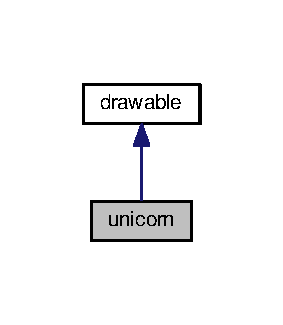
\includegraphics[width=136pt]{classunicorn__inherit__graph}
\end{center}
\end{figure}


Collaboration diagram for unicorn\+:\nopagebreak
\begin{figure}[H]
\begin{center}
\leavevmode
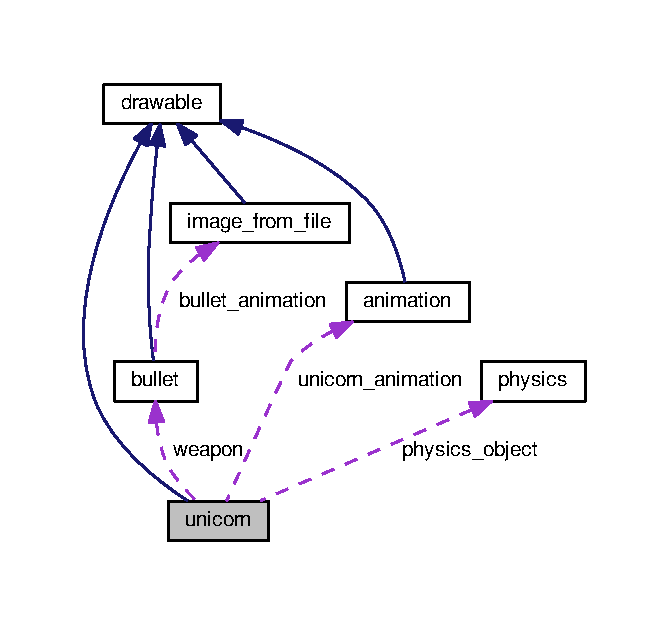
\includegraphics[width=350pt]{classunicorn__coll__graph}
\end{center}
\end{figure}
\subsection*{Public Member Functions}
\begin{DoxyCompactItemize}
\item 
\hyperlink{classunicorn_a89d3654cfd56c282b5061082e6864245}{unicorn} (sf\+::\+Vector2f position, std\+::string filename, std\+::string file\+\_\+rainbow, \hyperlink{typedefs_8hpp_a38f93e4749e0d65d51360c429766d212}{actions} \&actions\+\_\+array, \hyperlink{typedefs_8hpp_a7e1a7f34f6d09dabb4cdafd6e4118603}{collisions} \&the\+\_\+collisions, std\+::vector$<$ \hyperlink{typedefs_8hpp_a09ee7f853fc9bc830a9445a06fd53d4b}{mob\+\_\+ptr} $>$ \&all\+\_\+mobs, \hyperlink{typedefs_8hpp_a6c0fdb1dfd0c34dbbdbb5dcd3c608b07}{objects\+\_\+vector} \&objects, int \&Level\+\_\+counter, \hyperlink{classsoundtrack}{soundtrack} \&soundbuffer)
\begin{DoxyCompactList}\small\item\em Constructor to initialize the unicorn. \end{DoxyCompactList}\item 
void \hyperlink{classunicorn_a570c34d5669a8d2a61bdc1481e6f9dee}{draw} (sf\+::\+Render\+Window \&window) override
\begin{DoxyCompactList}\small\item\em function that draws the image \end{DoxyCompactList}\item 
void \hyperlink{classunicorn_a162f200a68342f7bc0baaf17c8cf3f9f}{move} (sf\+::\+Vector2f delta) override
\begin{DoxyCompactList}\small\item\em function that moves image object with a certian delta \end{DoxyCompactList}\item 
void \hyperlink{classunicorn_a07d5ca4e66632c0e871221a27146805a}{jump} () override
\begin{DoxyCompactList}\small\item\em let the unicorn jump \end{DoxyCompactList}\item 
sf\+::\+Float\+Rect \hyperlink{classunicorn_a1bac09fc59b04f14f5a093bc4daa04da}{get\+Global\+Bounds} () override
\begin{DoxyCompactList}\small\item\em function that gets the boundingbox of the image \end{DoxyCompactList}\item 
void \hyperlink{classunicorn_aadb47a9981c46d6add8704074df117df}{run\+\_\+actions} (\hyperlink{typedefs_8hpp_aab5add95f06d2ba25dbfed8eb07274fa}{object\+\_\+ptr} object) override
\begin{DoxyCompactList}\small\item\em functions that runs through all actions related to the unicorn \end{DoxyCompactList}\item 
\hyperlink{structcollision}{collision} \hyperlink{classunicorn_a40fe782f273abf46f6121db9aa4bf77a}{check\+\_\+for\+\_\+collisions} (char c) override
\begin{DoxyCompactList}\small\item\em Check the collisions vector. \end{DoxyCompactList}\item 
void \hyperlink{classunicorn_af448a3fa5fc5f09254b50afa151ce42b}{shoot} (sf\+::\+Vector2f fire\+\_\+position, sf\+::\+Render\+Window \&window, sf\+::\+Vector2f offset)
\begin{DoxyCompactList}\small\item\em function that shoots bullet \end{DoxyCompactList}\item 
void \hyperlink{classunicorn_af0e2581c426b4b1e32f8a7b484b4e242}{set\+\_\+spawn\+\_\+location} (sf\+::\+Vector2f new\+\_\+location)
\begin{DoxyCompactList}\small\item\em set the spawn location \end{DoxyCompactList}\item 
void \hyperlink{classunicorn_a8b5a22ab1b26daa540ceb09b5b5747d8}{damage} (\hyperlink{typedefs_8hpp_a09ee7f853fc9bc830a9445a06fd53d4b}{mob\+\_\+ptr} other)
\begin{DoxyCompactList}\small\item\em Do damage to the unicorn. \end{DoxyCompactList}\end{DoxyCompactItemize}
\subsection*{Private Attributes}
\begin{DoxyCompactItemize}
\item 
\mbox{\Hypertarget{classunicorn_a4a032891da1aa855b0b46c6e0b969a35}\label{classunicorn_a4a032891da1aa855b0b46c6e0b969a35}} 
bool {\bfseries going\+\_\+left} = false
\item 
\mbox{\Hypertarget{classunicorn_a7f4c9e68841d896da696132113602019}\label{classunicorn_a7f4c9e68841d896da696132113602019}} 
int {\bfseries jump\+\_\+counter} = 0
\item 
\mbox{\Hypertarget{classunicorn_a7673cbdfe14f719f710df4b324f74484}\label{classunicorn_a7673cbdfe14f719f710df4b324f74484}} 
int {\bfseries shoot\+\_\+timeout} = 0
\item 
\mbox{\Hypertarget{classunicorn_ab0462e46c2393f0bc0f5b2faa0b7b091}\label{classunicorn_ab0462e46c2393f0bc0f5b2faa0b7b091}} 
int {\bfseries lives} = 3
\item 
\mbox{\Hypertarget{classunicorn_a1cc767e234ec6d55ca0b576747f8d7d7}\label{classunicorn_a1cc767e234ec6d55ca0b576747f8d7d7}} 
\hyperlink{typedefs_8hpp_a38f93e4749e0d65d51360c429766d212}{actions} \& {\bfseries actions\+\_\+array}
\item 
\mbox{\Hypertarget{classunicorn_a0d6df4ae413adcf9307c2f36e9c1d51b}\label{classunicorn_a0d6df4ae413adcf9307c2f36e9c1d51b}} 
\hyperlink{classanimation}{animation} {\bfseries unicorn\+\_\+animation}
\item 
\mbox{\Hypertarget{classunicorn_a178463b08cbb4109fee0d37b4cb98d4f}\label{classunicorn_a178463b08cbb4109fee0d37b4cb98d4f}} 
\hyperlink{classanimation}{animation} {\bfseries rainbow}
\item 
\mbox{\Hypertarget{classunicorn_accaf554299ce27905fa8c47f602b0e98}\label{classunicorn_accaf554299ce27905fa8c47f602b0e98}} 
\hyperlink{classphysics}{physics} {\bfseries physics\+\_\+object}
\item 
\mbox{\Hypertarget{classunicorn_a77b6bd58d4bd308c55a530c50fdcce41}\label{classunicorn_a77b6bd58d4bd308c55a530c50fdcce41}} 
\hyperlink{typedefs_8hpp_a7e1a7f34f6d09dabb4cdafd6e4118603}{collisions} \& {\bfseries the\+\_\+collisions}
\item 
\mbox{\Hypertarget{classunicorn_ab16638b1ce0d1a7a0da9ecffc6370e8c}\label{classunicorn_ab16638b1ce0d1a7a0da9ecffc6370e8c}} 
sf\+::\+Vector2f {\bfseries spawn\+\_\+location}
\item 
\mbox{\Hypertarget{classunicorn_aac73bd105ef4ee4c7d46727a7e832bcf}\label{classunicorn_aac73bd105ef4ee4c7d46727a7e832bcf}} 
std\+::vector$<$ \hyperlink{typedefs_8hpp_a09ee7f853fc9bc830a9445a06fd53d4b}{mob\+\_\+ptr} $>$ \& {\bfseries all\+\_\+mobs}
\item 
\mbox{\Hypertarget{classunicorn_a3e51a9e196533b27304f21eb26d8f4ba}\label{classunicorn_a3e51a9e196533b27304f21eb26d8f4ba}} 
\hyperlink{classbullet}{bullet} {\bfseries weapon}
\item 
\mbox{\Hypertarget{classunicorn_ab808840ba1e83cb34c691ba2472d6f9b}\label{classunicorn_ab808840ba1e83cb34c691ba2472d6f9b}} 
bool {\bfseries got\+\_\+hit} = false
\item 
\mbox{\Hypertarget{classunicorn_ac0762399be7cd26263456d86fd2774ff}\label{classunicorn_ac0762399be7cd26263456d86fd2774ff}} 
int {\bfseries mob\+\_\+touch\+\_\+counter} = 0
\item 
\mbox{\Hypertarget{classunicorn_ac4e77e1b0fa4f0812cce288f5d90897b}\label{classunicorn_ac4e77e1b0fa4f0812cce288f5d90897b}} 
sf\+::\+Font {\bfseries font}
\item 
\mbox{\Hypertarget{classunicorn_a141d43a06ed4ba77c0aa891e0cf01b73}\label{classunicorn_a141d43a06ed4ba77c0aa891e0cf01b73}} 
sf\+::\+Text {\bfseries text}
\item 
\mbox{\Hypertarget{classunicorn_a7e53b65e44f4909ecedda128161673b6}\label{classunicorn_a7e53b65e44f4909ecedda128161673b6}} 
int {\bfseries text\+\_\+counter} = 0
\item 
\mbox{\Hypertarget{classunicorn_a4b92a71eb730de05a72d7963bfe13254}\label{classunicorn_a4b92a71eb730de05a72d7963bfe13254}} 
int \& {\bfseries level\+\_\+counter}
\item 
\mbox{\Hypertarget{classunicorn_a1aa49dd70ca2165a228c02d63e6d3217}\label{classunicorn_a1aa49dd70ca2165a228c02d63e6d3217}} 
\hyperlink{classsoundtrack}{soundtrack} \& {\bfseries soundbuffer}
\item 
\mbox{\Hypertarget{classunicorn_ae1f8f06df0010b0d469c3e56bb67c301}\label{classunicorn_ae1f8f06df0010b0d469c3e56bb67c301}} 
sf\+::\+Sound\+Buffer {\bfseries shootbuffer}
\end{DoxyCompactItemize}
\subsection*{Additional Inherited Members}


\subsection{Detailed Description}
class that is used to display and control the unicorn 

This class is used to control the unicorn and can be used to control it aswell (moving around and jumping. This class inherents the drawable class and has an object of the \hyperlink{classimage__from__file}{image\+\_\+from\+\_\+file} class.

\begin{DoxyDate}{Date}
19-\/01-\/2017 
\end{DoxyDate}


\subsection{Constructor \& Destructor Documentation}
\mbox{\Hypertarget{classunicorn_a89d3654cfd56c282b5061082e6864245}\label{classunicorn_a89d3654cfd56c282b5061082e6864245}} 
\index{unicorn@{unicorn}!unicorn@{unicorn}}
\index{unicorn@{unicorn}!unicorn@{unicorn}}
\subsubsection{\texorpdfstring{unicorn()}{unicorn()}}
{\footnotesize\ttfamily unicorn\+::unicorn (\begin{DoxyParamCaption}\item[{sf\+::\+Vector2f}]{position,  }\item[{std\+::string}]{filename,  }\item[{std\+::string}]{file\+\_\+rainbow,  }\item[{\hyperlink{typedefs_8hpp_a38f93e4749e0d65d51360c429766d212}{actions} \&}]{actions\+\_\+array,  }\item[{\hyperlink{typedefs_8hpp_a7e1a7f34f6d09dabb4cdafd6e4118603}{collisions} \&}]{the\+\_\+collisions,  }\item[{std\+::vector$<$ \hyperlink{typedefs_8hpp_a09ee7f853fc9bc830a9445a06fd53d4b}{mob\+\_\+ptr} $>$ \&}]{all\+\_\+mobs,  }\item[{\hyperlink{typedefs_8hpp_a6c0fdb1dfd0c34dbbdbb5dcd3c608b07}{objects\+\_\+vector} \&}]{objects,  }\item[{int \&}]{Level\+\_\+counter,  }\item[{\hyperlink{classsoundtrack}{soundtrack} \&}]{soundbuffer }\end{DoxyParamCaption})}



Constructor to initialize the unicorn. 

This construcor initializes the position of the unicorn as well a the filename of the image used


\begin{DoxyParams}[1]{Parameters}
\mbox{\tt in}  & {\em position} & Position where the image is placed \\
\hline
\mbox{\tt in}  & {\em filename} & The filename of the image \\
\hline
\mbox{\tt in}  & {\em actions\+\_\+array} & The actions of the unicorn \\
\hline
\mbox{\tt in}  & {\em the\+\_\+collisions} & The collisions the unicorn has \\
\hline
\mbox{\tt in}  & {\em all\+\_\+mobs} & All mobs in level \mbox{[}in\mbox{]} objects all walls/obstacles that unicorn and bullet can react to \\
\hline
\end{DoxyParams}


\subsection{Member Function Documentation}
\mbox{\Hypertarget{classunicorn_a40fe782f273abf46f6121db9aa4bf77a}\label{classunicorn_a40fe782f273abf46f6121db9aa4bf77a}} 
\index{unicorn@{unicorn}!check\+\_\+for\+\_\+collisions@{check\+\_\+for\+\_\+collisions}}
\index{check\+\_\+for\+\_\+collisions@{check\+\_\+for\+\_\+collisions}!unicorn@{unicorn}}
\subsubsection{\texorpdfstring{check\+\_\+for\+\_\+collisions()}{check\_for\_collisions()}}
{\footnotesize\ttfamily \hyperlink{structcollision}{collision} unicorn\+::check\+\_\+for\+\_\+collisions (\begin{DoxyParamCaption}\item[{char}]{c }\end{DoxyParamCaption})\hspace{0.3cm}{\ttfamily [override]}, {\ttfamily [virtual]}}



Check the collisions vector. 

This function checks the collisions vector for a collision where the c is the direction. When c is \textquotesingle{}U\textquotesingle{} it checks the U value of the collisions struct.


\begin{DoxyParams}[1]{Parameters}
\mbox{\tt in}  & {\em c} & The character to check for \\
\hline
\end{DoxyParams}


Reimplemented from \hyperlink{classdrawable_abbc6e0089d502ba48c3fcb9c96e3966e}{drawable}.

\mbox{\Hypertarget{classunicorn_a8b5a22ab1b26daa540ceb09b5b5747d8}\label{classunicorn_a8b5a22ab1b26daa540ceb09b5b5747d8}} 
\index{unicorn@{unicorn}!damage@{damage}}
\index{damage@{damage}!unicorn@{unicorn}}
\subsubsection{\texorpdfstring{damage()}{damage()}}
{\footnotesize\ttfamily void unicorn\+::damage (\begin{DoxyParamCaption}\item[{\hyperlink{typedefs_8hpp_a09ee7f853fc9bc830a9445a06fd53d4b}{mob\+\_\+ptr}}]{other }\end{DoxyParamCaption})}



Do damage to the unicorn. 

This function does damage to the unicorn. It also sets a counter to get the unicorn to move back the way he came if he hits another mob. This is why it needs to get the position of that mob from a \hyperlink{typedefs_8hpp_a09ee7f853fc9bc830a9445a06fd53d4b}{mob\+\_\+ptr} given to the function as a parameter.


\begin{DoxyParams}[1]{Parameters}
\mbox{\tt in}  & {\em other} & The \hyperlink{typedefs_8hpp_a09ee7f853fc9bc830a9445a06fd53d4b}{mob\+\_\+ptr} that is doing damage to the unicorn \\
\hline
\end{DoxyParams}
\mbox{\Hypertarget{classunicorn_a570c34d5669a8d2a61bdc1481e6f9dee}\label{classunicorn_a570c34d5669a8d2a61bdc1481e6f9dee}} 
\index{unicorn@{unicorn}!draw@{draw}}
\index{draw@{draw}!unicorn@{unicorn}}
\subsubsection{\texorpdfstring{draw()}{draw()}}
{\footnotesize\ttfamily void unicorn\+::draw (\begin{DoxyParamCaption}\item[{sf\+::\+Render\+Window \&}]{window }\end{DoxyParamCaption})\hspace{0.3cm}{\ttfamily [override]}, {\ttfamily [virtual]}}



function that draws the image 

this function draws the unicorn, depending on the unicorn going left or rigth scales the image (if it isn\textquotesingle{}t already correctly scaled)


\begin{DoxyParams}[1]{Parameters}
\mbox{\tt in}  & {\em window} & S\+F\+ML window that is used to display the image \\
\hline
\end{DoxyParams}


Implements \hyperlink{classdrawable_a4e49e2c1121704c83ce24c5f48dd910f}{drawable}.

\mbox{\Hypertarget{classunicorn_a1bac09fc59b04f14f5a093bc4daa04da}\label{classunicorn_a1bac09fc59b04f14f5a093bc4daa04da}} 
\index{unicorn@{unicorn}!get\+Global\+Bounds@{get\+Global\+Bounds}}
\index{get\+Global\+Bounds@{get\+Global\+Bounds}!unicorn@{unicorn}}
\subsubsection{\texorpdfstring{get\+Global\+Bounds()}{getGlobalBounds()}}
{\footnotesize\ttfamily sf\+::\+Float\+Rect unicorn\+::get\+Global\+Bounds (\begin{DoxyParamCaption}{ }\end{DoxyParamCaption})\hspace{0.3cm}{\ttfamily [override]}, {\ttfamily [virtual]}}



function that gets the boundingbox of the image 

This function gets the boundingbox of the image and returns this.

\begin{DoxyReturn}{Returns}
wich are the boundaries of the image 
\end{DoxyReturn}


Implements \hyperlink{classdrawable_ae013ac0be47538be9ce885d6642daf73}{drawable}.

\mbox{\Hypertarget{classunicorn_a07d5ca4e66632c0e871221a27146805a}\label{classunicorn_a07d5ca4e66632c0e871221a27146805a}} 
\index{unicorn@{unicorn}!jump@{jump}}
\index{jump@{jump}!unicorn@{unicorn}}
\subsubsection{\texorpdfstring{jump()}{jump()}}
{\footnotesize\ttfamily void unicorn\+::jump (\begin{DoxyParamCaption}{ }\end{DoxyParamCaption})\hspace{0.3cm}{\ttfamily [override]}, {\ttfamily [virtual]}}



let the unicorn jump 

This function allows the unicorn to jump if it is not already jumping and if the unicorn is standing on the ground.

\begin{DoxySeeAlso}{See also}
sf\+::\+Sprite\+::get\+Global\+Bounds() 
\end{DoxySeeAlso}


Reimplemented from \hyperlink{classdrawable_ac39691470b7874f5dec59efe649d3981}{drawable}.

\mbox{\Hypertarget{classunicorn_a162f200a68342f7bc0baaf17c8cf3f9f}\label{classunicorn_a162f200a68342f7bc0baaf17c8cf3f9f}} 
\index{unicorn@{unicorn}!move@{move}}
\index{move@{move}!unicorn@{unicorn}}
\subsubsection{\texorpdfstring{move()}{move()}}
{\footnotesize\ttfamily void unicorn\+::move (\begin{DoxyParamCaption}\item[{sf\+::\+Vector2f}]{delta }\end{DoxyParamCaption})\hspace{0.3cm}{\ttfamily [override]}, {\ttfamily [virtual]}}



function that moves image object with a certian delta 

This function moves the image with a certian vector. This vector is the parameter delta


\begin{DoxyParams}[1]{Parameters}
\mbox{\tt in}  & {\em delta} & sf\+::\+Vector2f that determines movement\\
\hline
\end{DoxyParams}
\begin{DoxySeeAlso}{See also}
\href{https://www.sfml-dev.org/documentation/2.0/classsf_1_1Transformable.php#ab9ca691522f6ddc1a40406849b87c469}{\tt https\+://www.\+sfml-\/dev.\+org/documentation/2.\+0/classsf\+\_\+1\+\_\+1\+Transformable.\+php\#ab9ca691522f6ddc1a40406849b87c469} 
\end{DoxySeeAlso}


Reimplemented from \hyperlink{classdrawable_ad0d3930c045cc6776aa2c3965be32491}{drawable}.

\mbox{\Hypertarget{classunicorn_aadb47a9981c46d6add8704074df117df}\label{classunicorn_aadb47a9981c46d6add8704074df117df}} 
\index{unicorn@{unicorn}!run\+\_\+actions@{run\+\_\+actions}}
\index{run\+\_\+actions@{run\+\_\+actions}!unicorn@{unicorn}}
\subsubsection{\texorpdfstring{run\+\_\+actions()}{run\_actions()}}
{\footnotesize\ttfamily void unicorn\+::run\+\_\+actions (\begin{DoxyParamCaption}\item[{\hyperlink{typedefs_8hpp_aab5add95f06d2ba25dbfed8eb07274fa}{object\+\_\+ptr}}]{object }\end{DoxyParamCaption})\hspace{0.3cm}{\ttfamily [override]}, {\ttfamily [virtual]}}



functions that runs through all actions related to the unicorn 

This function contains for-\/loop that runs through actions for this unicorn 

Reimplemented from \hyperlink{classdrawable_a715df01a318331e5611a2b0ad30109ff}{drawable}.

\mbox{\Hypertarget{classunicorn_af0e2581c426b4b1e32f8a7b484b4e242}\label{classunicorn_af0e2581c426b4b1e32f8a7b484b4e242}} 
\index{unicorn@{unicorn}!set\+\_\+spawn\+\_\+location@{set\+\_\+spawn\+\_\+location}}
\index{set\+\_\+spawn\+\_\+location@{set\+\_\+spawn\+\_\+location}!unicorn@{unicorn}}
\subsubsection{\texorpdfstring{set\+\_\+spawn\+\_\+location()}{set\_spawn\_location()}}
{\footnotesize\ttfamily void unicorn\+::set\+\_\+spawn\+\_\+location (\begin{DoxyParamCaption}\item[{sf\+::\+Vector2f}]{new\+\_\+location }\end{DoxyParamCaption})}



set the spawn location 

This function sets the spawn location of the unicorn to a new location. The unicorn will spawn in the new location if he dies.


\begin{DoxyParams}[1]{Parameters}
\mbox{\tt in}  & {\em new\+\_\+location} & The new spawn location for the unicorn \\
\hline
\end{DoxyParams}
\mbox{\Hypertarget{classunicorn_af448a3fa5fc5f09254b50afa151ce42b}\label{classunicorn_af448a3fa5fc5f09254b50afa151ce42b}} 
\index{unicorn@{unicorn}!shoot@{shoot}}
\index{shoot@{shoot}!unicorn@{unicorn}}
\subsubsection{\texorpdfstring{shoot()}{shoot()}}
{\footnotesize\ttfamily void unicorn\+::shoot (\begin{DoxyParamCaption}\item[{sf\+::\+Vector2f}]{fire\+\_\+position,  }\item[{sf\+::\+Render\+Window \&}]{window,  }\item[{sf\+::\+Vector2f}]{offset }\end{DoxyParamCaption})}



function that shoots bullet 

This function is used to fire a bullet object. Given the start position , a window to draw on and the offset it should be fired with. When user presses the L\+Control button the shoot\+\_\+timeout is set to 100. If not hit by something the bullet will disappear.


\begin{DoxyParams}[1]{Parameters}
\mbox{\tt in}  & {\em fire\+\_\+position} & position that the bullet is fired from \\
\hline
\mbox{\tt in}  & {\em window} & sf\+::\+Render\+Window to display bullet on \mbox{[}in\mbox{]} offset sf\+::\+Vector2f that decides wich way the bullet goes. \\
\hline
\end{DoxyParams}


The documentation for this class was generated from the following files\+:\begin{DoxyCompactItemize}
\item 
\hyperlink{unicorn_8hpp}{unicorn.\+hpp}\item 
unicorn.\+cpp\end{DoxyCompactItemize}

\hypertarget{classunknown__color}{}\section{unknown\+\_\+color Class Reference}
\label{classunknown__color}\index{unknown\+\_\+color@{unknown\+\_\+color}}


Unknown color error.  




{\ttfamily \#include $<$exceptions.\+hpp$>$}



Inheritance diagram for unknown\+\_\+color\+:\nopagebreak
\begin{figure}[H]
\begin{center}
\leavevmode
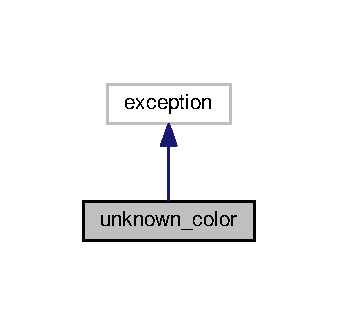
\includegraphics[width=162pt]{classunknown__color__inherit__graph}
\end{center}
\end{figure}


Collaboration diagram for unknown\+\_\+color\+:\nopagebreak
\begin{figure}[H]
\begin{center}
\leavevmode
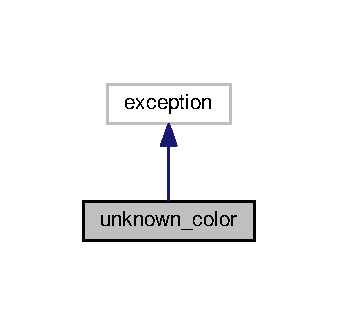
\includegraphics[width=162pt]{classunknown__color__coll__graph}
\end{center}
\end{figure}
\subsection*{Public Member Functions}
\begin{DoxyCompactItemize}
\item 
\hyperlink{classunknown__color_aef7c5513b511dd59ba1a3a58798966d3}{unknown\+\_\+color} (const std\+::string color)
\begin{DoxyCompactList}\small\item\em Constructor. \end{DoxyCompactList}\item 
const char $\ast$ \hyperlink{classunknown__color_a3340e3af5b5f734727b73ddf25df3265}{what} () const noexcept override
\begin{DoxyCompactList}\small\item\em Return message. \end{DoxyCompactList}\end{DoxyCompactItemize}


\subsection{Detailed Description}
Unknown color error. 

This class is used to generate a unknown color exception. It inherrits the std\+::exception class so it can be easily caught with an try catch block.

\begin{DoxyDate}{Date}
26-\/1-\/2017 
\end{DoxyDate}


\subsection{Constructor \& Destructor Documentation}
\mbox{\Hypertarget{classunknown__color_aef7c5513b511dd59ba1a3a58798966d3}\label{classunknown__color_aef7c5513b511dd59ba1a3a58798966d3}} 
\index{unknown\+\_\+color@{unknown\+\_\+color}!unknown\+\_\+color@{unknown\+\_\+color}}
\index{unknown\+\_\+color@{unknown\+\_\+color}!unknown\+\_\+color@{unknown\+\_\+color}}
\subsubsection{\texorpdfstring{unknown\+\_\+color()}{unknown\_color()}}
{\footnotesize\ttfamily unknown\+\_\+color\+::unknown\+\_\+color (\begin{DoxyParamCaption}\item[{const std\+::string}]{color }\end{DoxyParamCaption})\hspace{0.3cm}{\ttfamily [inline]}}



Constructor. 

This constructor puts a message into a string and saves that as a private variable. The color is also added to the string.


\begin{DoxyParams}[1]{Parameters}
\mbox{\tt in}  & {\em color} & The name of the color \\
\hline
\end{DoxyParams}


\subsection{Member Function Documentation}
\mbox{\Hypertarget{classunknown__color_a3340e3af5b5f734727b73ddf25df3265}\label{classunknown__color_a3340e3af5b5f734727b73ddf25df3265}} 
\index{unknown\+\_\+color@{unknown\+\_\+color}!what@{what}}
\index{what@{what}!unknown\+\_\+color@{unknown\+\_\+color}}
\subsubsection{\texorpdfstring{what()}{what()}}
{\footnotesize\ttfamily const char$\ast$ unknown\+\_\+color\+::what (\begin{DoxyParamCaption}{ }\end{DoxyParamCaption}) const\hspace{0.3cm}{\ttfamily [inline]}, {\ttfamily [override]}, {\ttfamily [noexcept]}}



Return message. 

This function returns the message so it can be printed. It overrides the what function from the std\+::exception superclass, making it easy to capture.


\begin{DoxyRetVals}{Return values}
{\em const} & char $\ast$ \{The error message as a const char $\ast$\} \\
\hline
\end{DoxyRetVals}


The documentation for this class was generated from the following file\+:\begin{DoxyCompactItemize}
\item 
exceptions.\+hpp\end{DoxyCompactItemize}

\hypertarget{classunknown__type}{}\section{unknown\+\_\+type Class Reference}
\label{classunknown__type}\index{unknown\+\_\+type@{unknown\+\_\+type}}


Unknown type error.  




{\ttfamily \#include $<$exceptions.\+hpp$>$}



Inheritance diagram for unknown\+\_\+type\+:\nopagebreak
\begin{figure}[H]
\begin{center}
\leavevmode
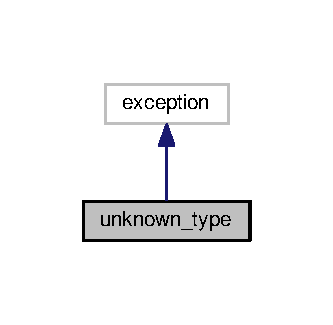
\includegraphics[width=160pt]{classunknown__type__inherit__graph}
\end{center}
\end{figure}


Collaboration diagram for unknown\+\_\+type\+:\nopagebreak
\begin{figure}[H]
\begin{center}
\leavevmode
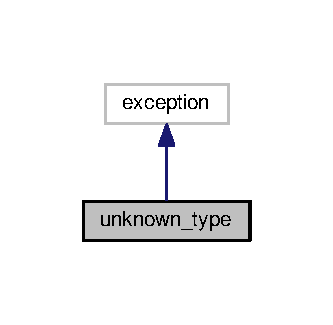
\includegraphics[width=160pt]{classunknown__type__coll__graph}
\end{center}
\end{figure}
\subsection*{Public Member Functions}
\begin{DoxyCompactItemize}
\item 
\hyperlink{classunknown__type_ad0900df174fd2897ea46896d46d4ce47}{unknown\+\_\+type} (const std\+::string type)
\begin{DoxyCompactList}\small\item\em constructor \end{DoxyCompactList}\item 
const char $\ast$ \hyperlink{classunknown__type_a95f8c551c7bf001353d4a68b6874650d}{what} () const noexcept override
\begin{DoxyCompactList}\small\item\em Return message. \end{DoxyCompactList}\end{DoxyCompactItemize}


\subsection{Detailed Description}
Unknown type error. 

This class is used to generate a unknown type error exception. It inherrits the std\+::exception class so it can be easily caught with an try catch block.

\begin{DoxyDate}{Date}
24-\/1-\/2017 
\end{DoxyDate}


\subsection{Constructor \& Destructor Documentation}
\mbox{\Hypertarget{classunknown__type_ad0900df174fd2897ea46896d46d4ce47}\label{classunknown__type_ad0900df174fd2897ea46896d46d4ce47}} 
\index{unknown\+\_\+type@{unknown\+\_\+type}!unknown\+\_\+type@{unknown\+\_\+type}}
\index{unknown\+\_\+type@{unknown\+\_\+type}!unknown\+\_\+type@{unknown\+\_\+type}}
\subsubsection{\texorpdfstring{unknown\+\_\+type()}{unknown\_type()}}
{\footnotesize\ttfamily unknown\+\_\+type\+::unknown\+\_\+type (\begin{DoxyParamCaption}\item[{const std\+::string}]{type }\end{DoxyParamCaption})\hspace{0.3cm}{\ttfamily [inline]}}



constructor 

This constructor puts a message into a string and saves that as a private variable. The type is also added to the string.


\begin{DoxyParams}[1]{Parameters}
\mbox{\tt in}  & {\em type} & The incorrect type that was received \\
\hline
\end{DoxyParams}


\subsection{Member Function Documentation}
\mbox{\Hypertarget{classunknown__type_a95f8c551c7bf001353d4a68b6874650d}\label{classunknown__type_a95f8c551c7bf001353d4a68b6874650d}} 
\index{unknown\+\_\+type@{unknown\+\_\+type}!what@{what}}
\index{what@{what}!unknown\+\_\+type@{unknown\+\_\+type}}
\subsubsection{\texorpdfstring{what()}{what()}}
{\footnotesize\ttfamily const char$\ast$ unknown\+\_\+type\+::what (\begin{DoxyParamCaption}{ }\end{DoxyParamCaption}) const\hspace{0.3cm}{\ttfamily [inline]}, {\ttfamily [override]}, {\ttfamily [noexcept]}}



Return message. 

This function returns the message so it can be printed. It overrides the what function from the std\+::exception superclass, making it easy to capture.


\begin{DoxyRetVals}{Return values}
{\em const} & char $\ast$ \{The error message as a const char $\ast$\} \\
\hline
\end{DoxyRetVals}


The documentation for this class was generated from the following file\+:\begin{DoxyCompactItemize}
\item 
\hyperlink{exceptions_8hpp}{exceptions.\+hpp}\end{DoxyCompactItemize}

\hypertarget{classwall}{}\section{wall Class Reference}
\label{classwall}\index{wall@{wall}}


Class for walls and platforms.  




{\ttfamily \#include $<$wall.\+hpp$>$}



Inheritance diagram for wall\+:\nopagebreak
\begin{figure}[H]
\begin{center}
\leavevmode
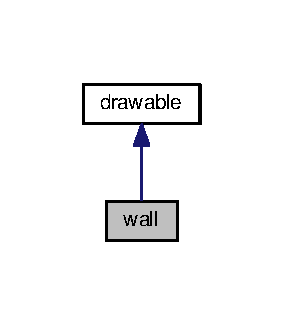
\includegraphics[width=136pt]{classwall__inherit__graph}
\end{center}
\end{figure}


Collaboration diagram for wall\+:\nopagebreak
\begin{figure}[H]
\begin{center}
\leavevmode
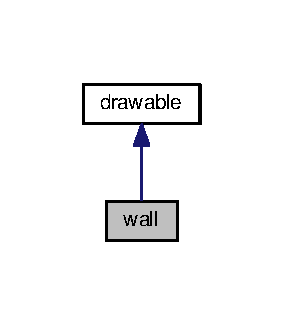
\includegraphics[width=136pt]{classwall__coll__graph}
\end{center}
\end{figure}
\subsection*{Public Member Functions}
\begin{DoxyCompactItemize}
\item 
\hyperlink{classwall_ac9c0db974e7839223fc4eb18c51dac62}{wall} (sf\+::\+Vector2f position, sf\+::\+Vector2f size, sf\+::\+Color object\+\_\+color, std\+::string image\+\_\+name=\char`\"{}\char`\"{})
\begin{DoxyCompactList}\small\item\em Constructor for a wall. \end{DoxyCompactList}\item 
void \hyperlink{classwall_aa25b8377e1d9a209fabd2271294f05d0}{draw} (sf\+::\+Render\+Window \&window) override
\begin{DoxyCompactList}\small\item\em Draw function for the wall. \end{DoxyCompactList}\item 
sf\+::\+Float\+Rect \hyperlink{classwall_a317a464c879cfdf9464bd6f1b62d9101}{get\+Global\+Bounds} () override
\begin{DoxyCompactList}\small\item\em Function that gives de global bounds. \end{DoxyCompactList}\item 
std\+::string \hyperlink{classwall_aab1de4f144f176b134a967ba08747932}{object\+\_\+information} () override
\begin{DoxyCompactList}\small\item\em Funtion that returns object information. \end{DoxyCompactList}\end{DoxyCompactItemize}
\subsection*{Additional Inherited Members}


\subsection{Detailed Description}
Class for walls and platforms. 

This class can be used for making rectangle shapes used as wall or platform for walking on or as boundry.

\begin{DoxyDate}{Date}
23/01/17 
\end{DoxyDate}


\subsection{Constructor \& Destructor Documentation}
\mbox{\Hypertarget{classwall_ac9c0db974e7839223fc4eb18c51dac62}\label{classwall_ac9c0db974e7839223fc4eb18c51dac62}} 
\index{wall@{wall}!wall@{wall}}
\index{wall@{wall}!wall@{wall}}
\subsubsection{\texorpdfstring{wall()}{wall()}}
{\footnotesize\ttfamily wall\+::wall (\begin{DoxyParamCaption}\item[{sf\+::\+Vector2f}]{position,  }\item[{sf\+::\+Vector2f}]{size,  }\item[{sf\+::\+Color}]{object\+\_\+color,  }\item[{std\+::string}]{image\+\_\+name = {\ttfamily \char`\"{}\char`\"{}} }\end{DoxyParamCaption})}



Constructor for a wall. 

Constructor that initializes position, size and color of drawable


\begin{DoxyParams}[1]{Parameters}
\mbox{\tt in}  & {\em position} & Position of drawable, this is a sf\+::\+Vector2f and const \\
\hline
\mbox{\tt in}  & {\em size} & Size of drawable, this is a sf\+::\+Vector2f and const \\
\hline
\mbox{\tt in}  & {\em object\+\_\+color} & Color of the wall, this is a sf\+::\+Color \\
\hline
\mbox{\tt in}  & {\em image\+\_\+name} & An image to put inside the wall. (not specifically needed) \\
\hline
\end{DoxyParams}
\begin{DoxyNote}{Note}
The image will become the color specified. 
\end{DoxyNote}


\subsection{Member Function Documentation}
\mbox{\Hypertarget{classwall_aa25b8377e1d9a209fabd2271294f05d0}\label{classwall_aa25b8377e1d9a209fabd2271294f05d0}} 
\index{wall@{wall}!draw@{draw}}
\index{draw@{draw}!wall@{wall}}
\subsubsection{\texorpdfstring{draw()}{draw()}}
{\footnotesize\ttfamily void wall\+::draw (\begin{DoxyParamCaption}\item[{sf\+::\+Render\+Window \&}]{window }\end{DoxyParamCaption})\hspace{0.3cm}{\ttfamily [override]}, {\ttfamily [virtual]}}



Draw function for the wall. 

This function draw the wall to the render of the window.


\begin{DoxyParams}[1]{Parameters}
\mbox{\tt in}  & {\em window} & The window to render the image on \\
\hline
\end{DoxyParams}


Implements \hyperlink{classdrawable_a4e49e2c1121704c83ce24c5f48dd910f}{drawable}.

\mbox{\Hypertarget{classwall_a317a464c879cfdf9464bd6f1b62d9101}\label{classwall_a317a464c879cfdf9464bd6f1b62d9101}} 
\index{wall@{wall}!get\+Global\+Bounds@{get\+Global\+Bounds}}
\index{get\+Global\+Bounds@{get\+Global\+Bounds}!wall@{wall}}
\subsubsection{\texorpdfstring{get\+Global\+Bounds()}{getGlobalBounds()}}
{\footnotesize\ttfamily sf\+::\+Float\+Rect wall\+::get\+Global\+Bounds (\begin{DoxyParamCaption}{ }\end{DoxyParamCaption})\hspace{0.3cm}{\ttfamily [override]}, {\ttfamily [virtual]}}



Function that gives de global bounds. 

This function returns the globalbounds. The return value can be used in collision checking.

\begin{DoxyReturn}{Returns}
The sf\+::floatrect of the wall object 
\end{DoxyReturn}


Implements \hyperlink{classdrawable_ae013ac0be47538be9ce885d6642daf73}{drawable}.

\mbox{\Hypertarget{classwall_aab1de4f144f176b134a967ba08747932}\label{classwall_aab1de4f144f176b134a967ba08747932}} 
\index{wall@{wall}!object\+\_\+information@{object\+\_\+information}}
\index{object\+\_\+information@{object\+\_\+information}!wall@{wall}}
\subsubsection{\texorpdfstring{object\+\_\+information()}{object\_information()}}
{\footnotesize\ttfamily std\+::string wall\+::object\+\_\+information (\begin{DoxyParamCaption}{ }\end{DoxyParamCaption})\hspace{0.3cm}{\ttfamily [override]}, {\ttfamily [virtual]}}



Funtion that returns object information. 

This function returns object information. It does so in the following way\+: \hyperlink{classdrawable_a2ed0f8bb53f33477f7722efa7bb24583}{drawable\+::object\+\_\+information()} + size + color + image\+\_\+name

Example\+: W\+A\+LL (2627.\+720947,2226.\+875000) (10.\+000000,10.\+000000) green grass.\+png

\begin{DoxyReturn}{Returns}
The string with all the information in the way of the example 
\end{DoxyReturn}


Reimplemented from \hyperlink{classdrawable_a2ed0f8bb53f33477f7722efa7bb24583}{drawable}.



The documentation for this class was generated from the following files\+:\begin{DoxyCompactItemize}
\item 
\hyperlink{wall_8hpp}{wall.\+hpp}\item 
wall.\+cpp\end{DoxyCompactItemize}

\chapter{File Documentation}
\hypertarget{animation_8hpp}{}\section{animation.\+hpp File Reference}
\label{animation_8hpp}\index{animation.\+hpp@{animation.\+hpp}}
{\ttfamily \#include \char`\"{}S\+F\+M\+L/\+Graphics.\+hpp\char`\"{}}\newline
{\ttfamily \#include $<$memory$>$}\newline
{\ttfamily \#include \char`\"{}drawable.\+hpp\char`\"{}}\newline
{\ttfamily \#include \char`\"{}exceptions.\+hpp\char`\"{}}\newline
Include dependency graph for animation.\+hpp\+:
\nopagebreak
\begin{figure}[H]
\begin{center}
\leavevmode
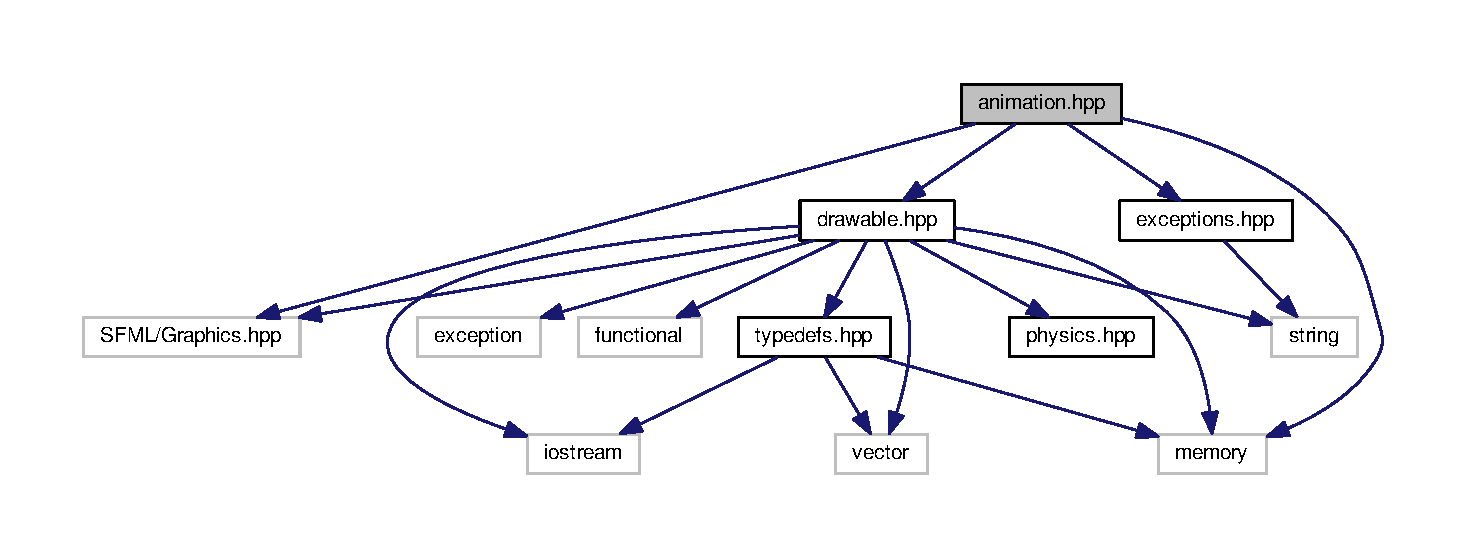
\includegraphics[width=350pt]{animation_8hpp__incl}
\end{center}
\end{figure}
This graph shows which files directly or indirectly include this file\+:
\nopagebreak
\begin{figure}[H]
\begin{center}
\leavevmode
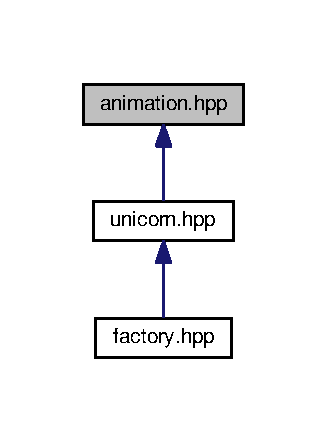
\includegraphics[width=304pt]{animation_8hpp__dep__incl}
\end{center}
\end{figure}
\subsection*{Classes}
\begin{DoxyCompactItemize}
\item 
class \hyperlink{classanimation}{animation}
\begin{DoxyCompactList}\small\item\em create sprite on screen with animations \end{DoxyCompactList}\end{DoxyCompactItemize}

\hypertarget{background_8hpp}{}\section{background.\+hpp File Reference}
\label{background_8hpp}\index{background.\+hpp@{background.\+hpp}}
{\ttfamily \#include $<$S\+F\+M\+L/\+Graphics.\+hpp$>$}\\*
{\ttfamily \#include \char`\"{}image.\+hpp\char`\"{}}\\*
{\ttfamily \#include $<$iostream$>$}\\*
{\ttfamily \#include $<$string$>$}\\*
Include dependency graph for background.\+hpp\+:\nopagebreak
\begin{figure}[H]
\begin{center}
\leavevmode
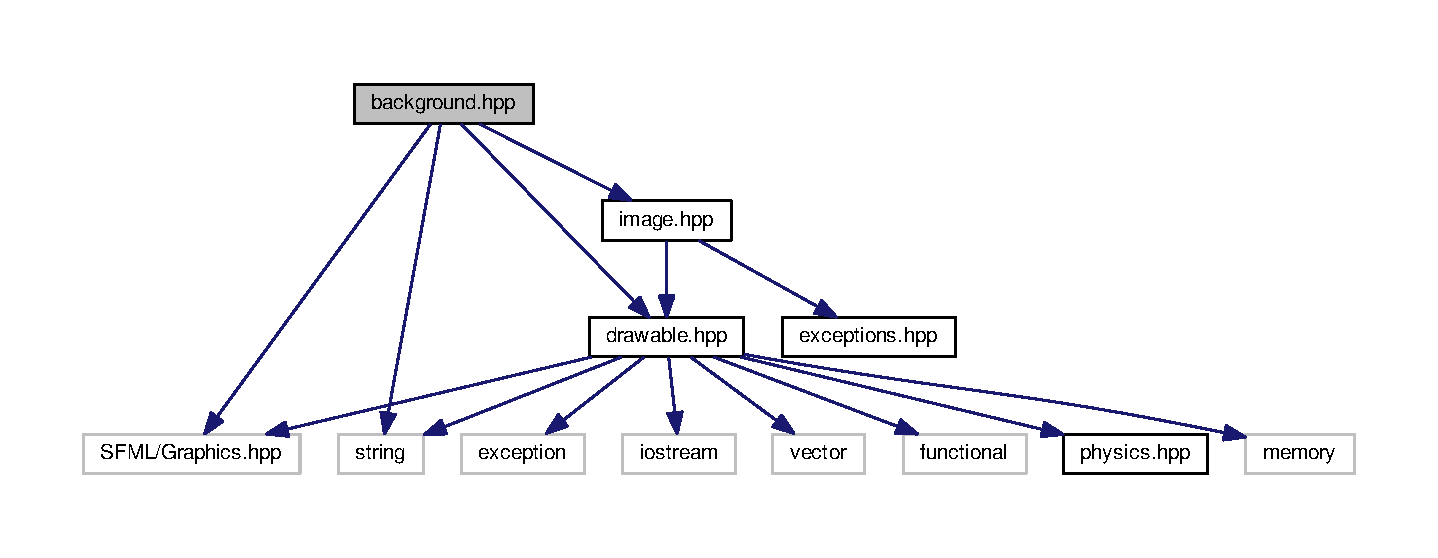
\includegraphics[width=350pt]{background_8hpp__incl}
\end{center}
\end{figure}
\subsection*{Classes}
\begin{DoxyCompactItemize}
\item 
class \hyperlink{class_background}{Background}
\begin{DoxyCompactList}\small\item\em Class that draws a background. \end{DoxyCompactList}\end{DoxyCompactItemize}

\hypertarget{base__level_8hpp}{}\section{base\+\_\+level.\+hpp File Reference}
\label{base__level_8hpp}\index{base\+\_\+level.\+hpp@{base\+\_\+level.\+hpp}}
{\ttfamily \#include \char`\"{}wall.\+hpp\char`\"{}}\newline
Include dependency graph for base\+\_\+level.\+hpp\+:\nopagebreak
\begin{figure}[H]
\begin{center}
\leavevmode
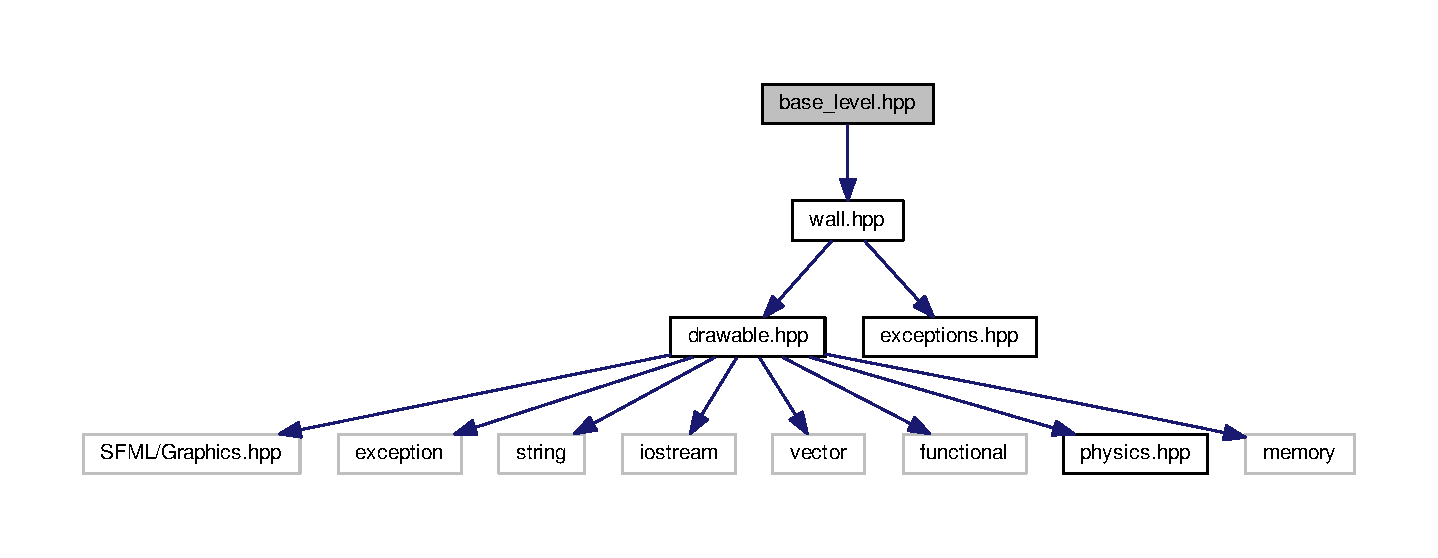
\includegraphics[width=350pt]{base__level_8hpp__incl}
\end{center}
\end{figure}
\subsection*{Classes}
\begin{DoxyCompactItemize}
\item 
class \hyperlink{classbase__level}{base\+\_\+level}
\begin{DoxyCompactList}\small\item\em level border creation class \end{DoxyCompactList}\end{DoxyCompactItemize}

\hypertarget{bullet_8hpp}{}\section{bullet.\+hpp File Reference}
\label{bullet_8hpp}\index{bullet.\+hpp@{bullet.\+hpp}}
{\ttfamily \#include \char`\"{}drawable.\+hpp\char`\"{}}\newline
{\ttfamily \#include \char`\"{}image.\+hpp\char`\"{}}\newline
{\ttfamily \#include \char`\"{}npc.\+hpp\char`\"{}}\newline
Include dependency graph for bullet.\+hpp\+:
\nopagebreak
\begin{figure}[H]
\begin{center}
\leavevmode
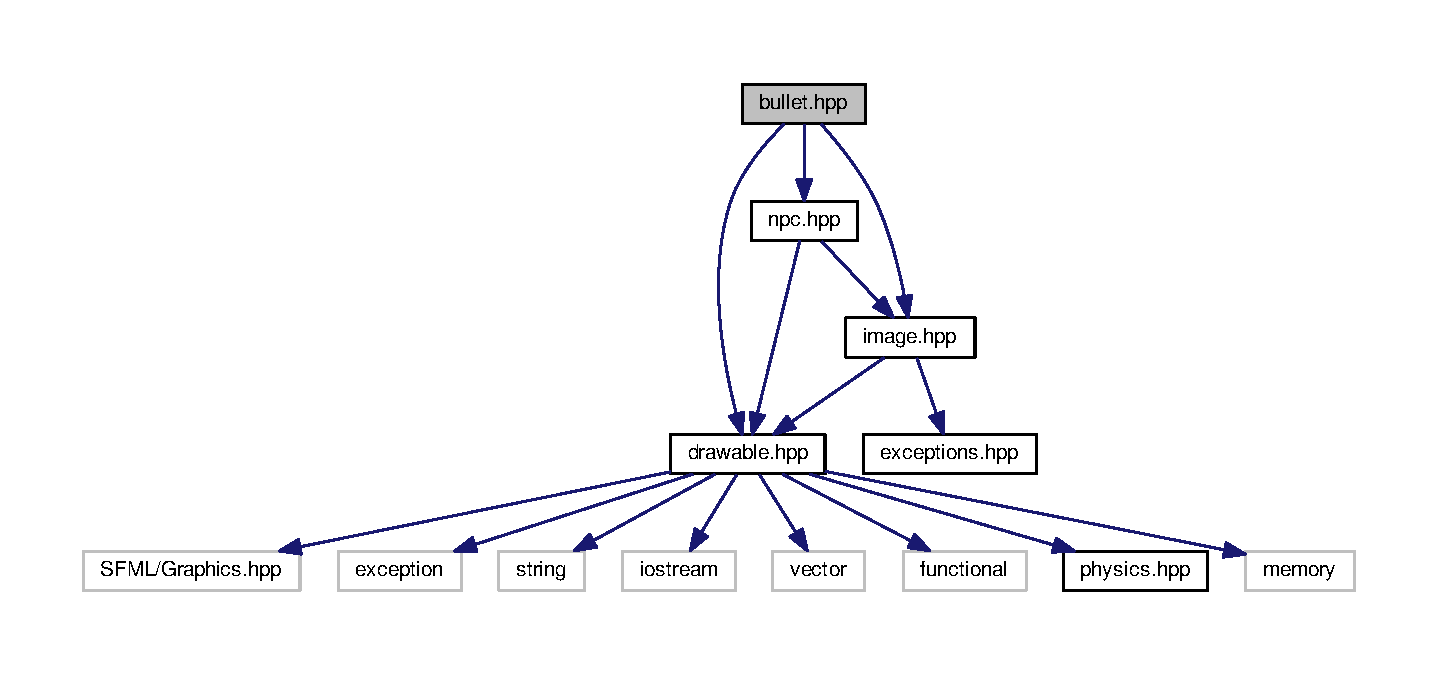
\includegraphics[width=350pt]{bullet_8hpp__incl}
\end{center}
\end{figure}
This graph shows which files directly or indirectly include this file\+:\nopagebreak
\begin{figure}[H]
\begin{center}
\leavevmode
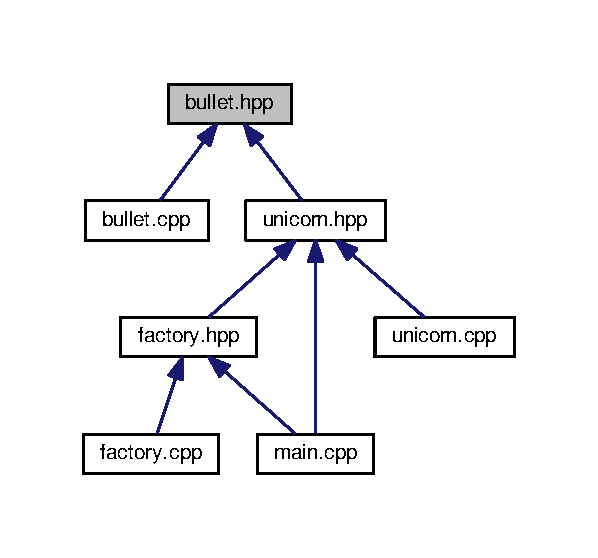
\includegraphics[width=147pt]{bullet_8hpp__dep__incl}
\end{center}
\end{figure}
\subsection*{Classes}
\begin{DoxyCompactItemize}
\item 
class \hyperlink{classbullet}{bullet}
\begin{DoxyCompactList}\small\item\em class calculates projectile to kill mobs \end{DoxyCompactList}\end{DoxyCompactItemize}

\hypertarget{button_8hpp}{}\section{button.\+hpp File Reference}
\label{button_8hpp}\index{button.\+hpp@{button.\+hpp}}
{\ttfamily \#include $<$S\+F\+M\+L/\+Graphics.\+hpp$>$}\newline
{\ttfamily \#include $<$iostream$>$}\newline
{\ttfamily \#include \char`\"{}drawable.\+hpp\char`\"{}}\newline
{\ttfamily \#include \char`\"{}image.\+hpp\char`\"{}}\newline
Include dependency graph for button.\+hpp\+:\nopagebreak
\begin{figure}[H]
\begin{center}
\leavevmode
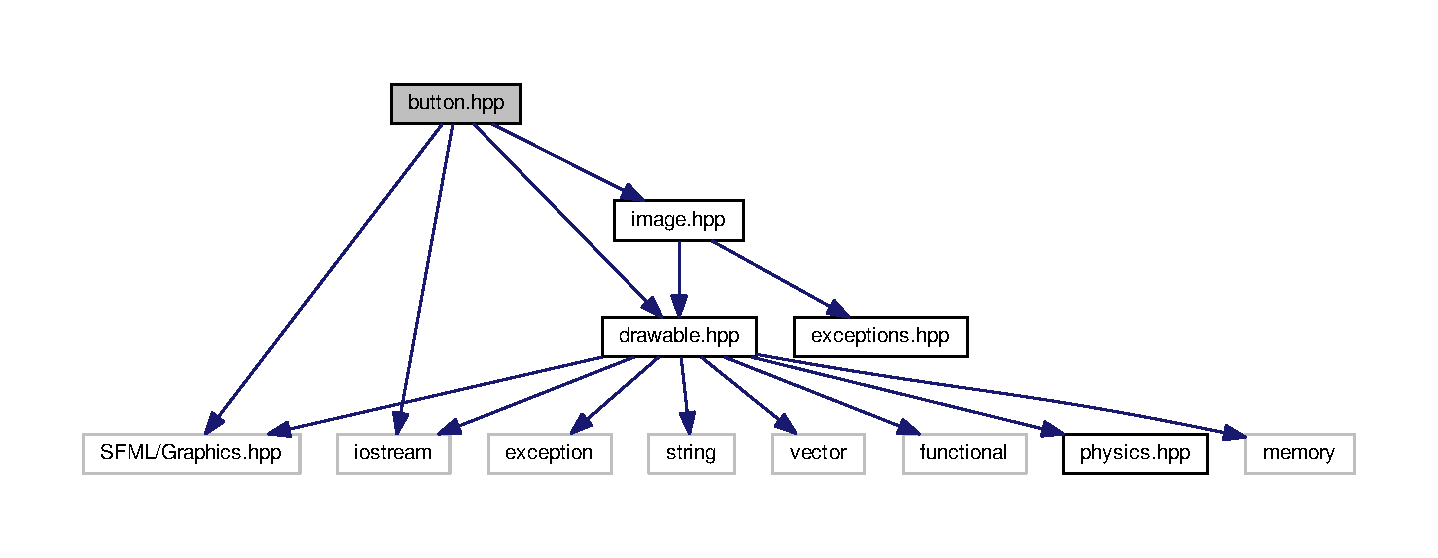
\includegraphics[width=350pt]{button_8hpp__incl}
\end{center}
\end{figure}
This graph shows which files directly or indirectly include this file\+:\nopagebreak
\begin{figure}[H]
\begin{center}
\leavevmode
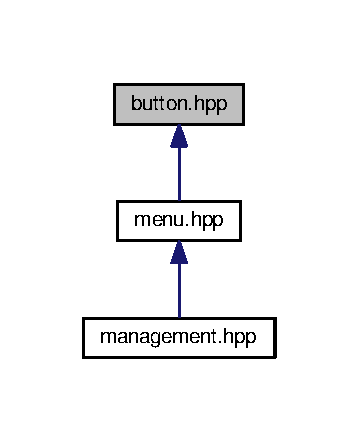
\includegraphics[width=172pt]{button_8hpp__dep__incl}
\end{center}
\end{figure}
\subsection*{Classes}
\begin{DoxyCompactItemize}
\item 
class \hyperlink{class_button}{Button}
\begin{DoxyCompactList}\small\item\em Creates a button at a specific place on the screen. \end{DoxyCompactList}\end{DoxyCompactItemize}

\hypertarget{camera_8hpp}{}\section{camera.\+hpp File Reference}
\label{camera_8hpp}\index{camera.\+hpp@{camera.\+hpp}}
{\ttfamily \#include $<$S\+F\+M\+L/\+Graphics.\+hpp$>$}\newline
{\ttfamily \#include $<$iostream$>$}\newline
{\ttfamily \#include \char`\"{}drawable.\+hpp\char`\"{}}\newline
Include dependency graph for camera.\+hpp\+:\nopagebreak
\begin{figure}[H]
\begin{center}
\leavevmode
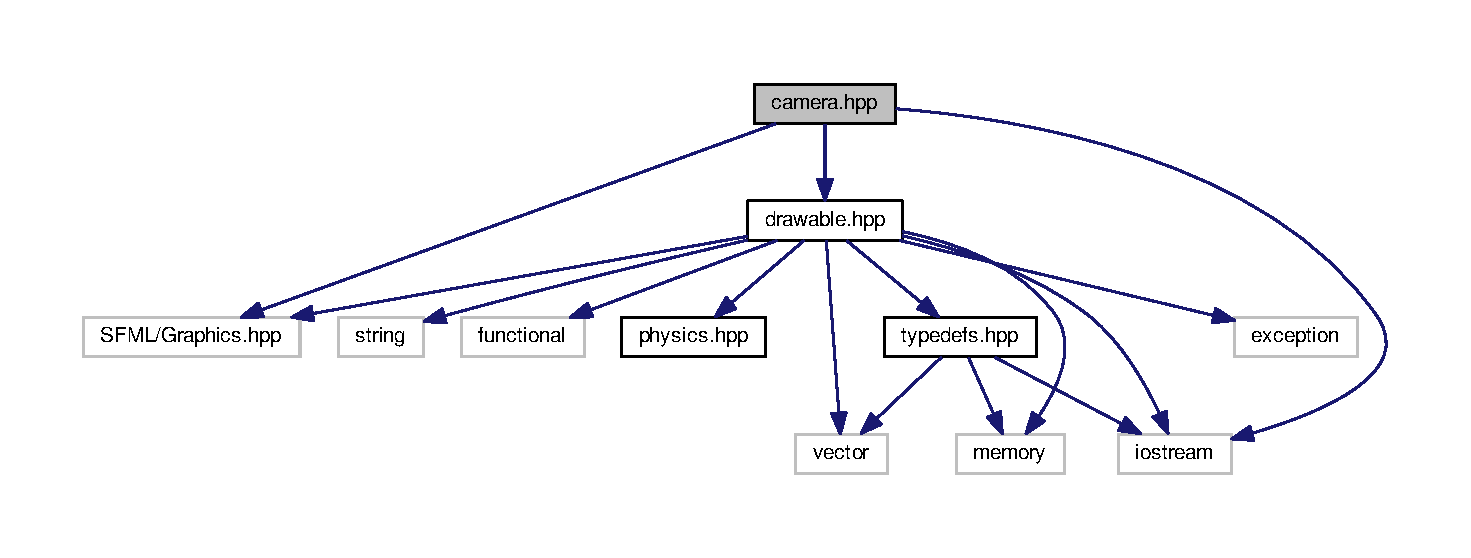
\includegraphics[width=350pt]{camera_8hpp__incl}
\end{center}
\end{figure}
\subsection*{Classes}
\begin{DoxyCompactItemize}
\item 
class \hyperlink{classcamera}{camera}
\begin{DoxyCompactList}\small\item\em object folowing camera \end{DoxyCompactList}\end{DoxyCompactItemize}

\hypertarget{drawable_8hpp}{}\section{drawable.\+hpp File Reference}
\label{drawable_8hpp}\index{drawable.\+hpp@{drawable.\+hpp}}
{\ttfamily \#include $<$S\+F\+M\+L/\+Graphics.\+hpp$>$}\newline
{\ttfamily \#include $<$exception$>$}\newline
{\ttfamily \#include $<$string$>$}\newline
{\ttfamily \#include $<$iostream$>$}\newline
{\ttfamily \#include $<$vector$>$}\newline
{\ttfamily \#include $<$functional$>$}\newline
{\ttfamily \#include \char`\"{}physics.\+hpp\char`\"{}}\newline
{\ttfamily \#include $<$memory$>$}\newline
Include dependency graph for drawable.\+hpp\+:\nopagebreak
\begin{figure}[H]
\begin{center}
\leavevmode
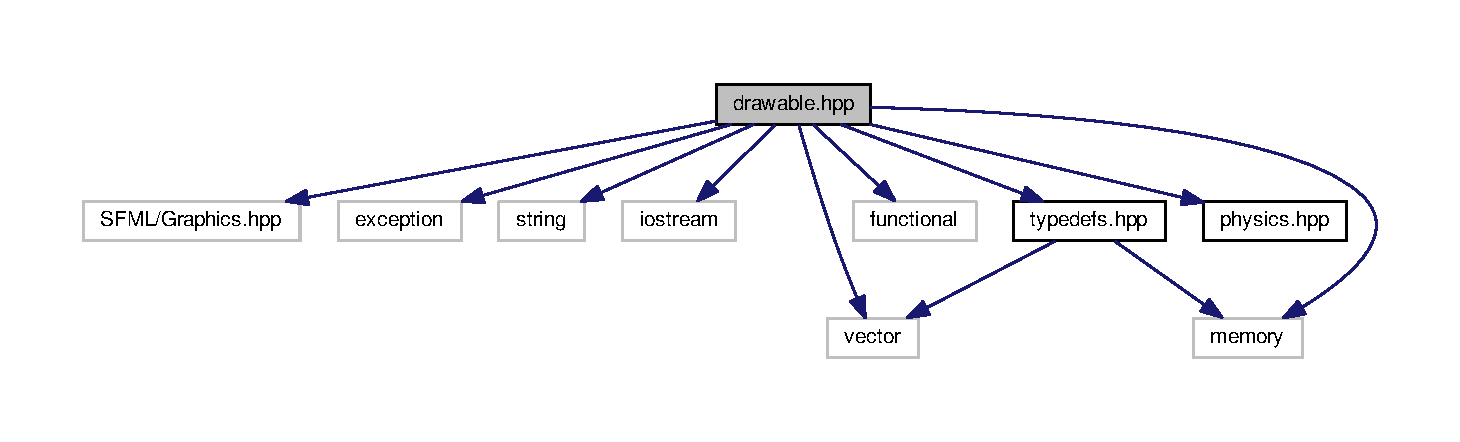
\includegraphics[width=350pt]{drawable_8hpp__incl}
\end{center}
\end{figure}
This graph shows which files directly or indirectly include this file\+:\nopagebreak
\begin{figure}[H]
\begin{center}
\leavevmode
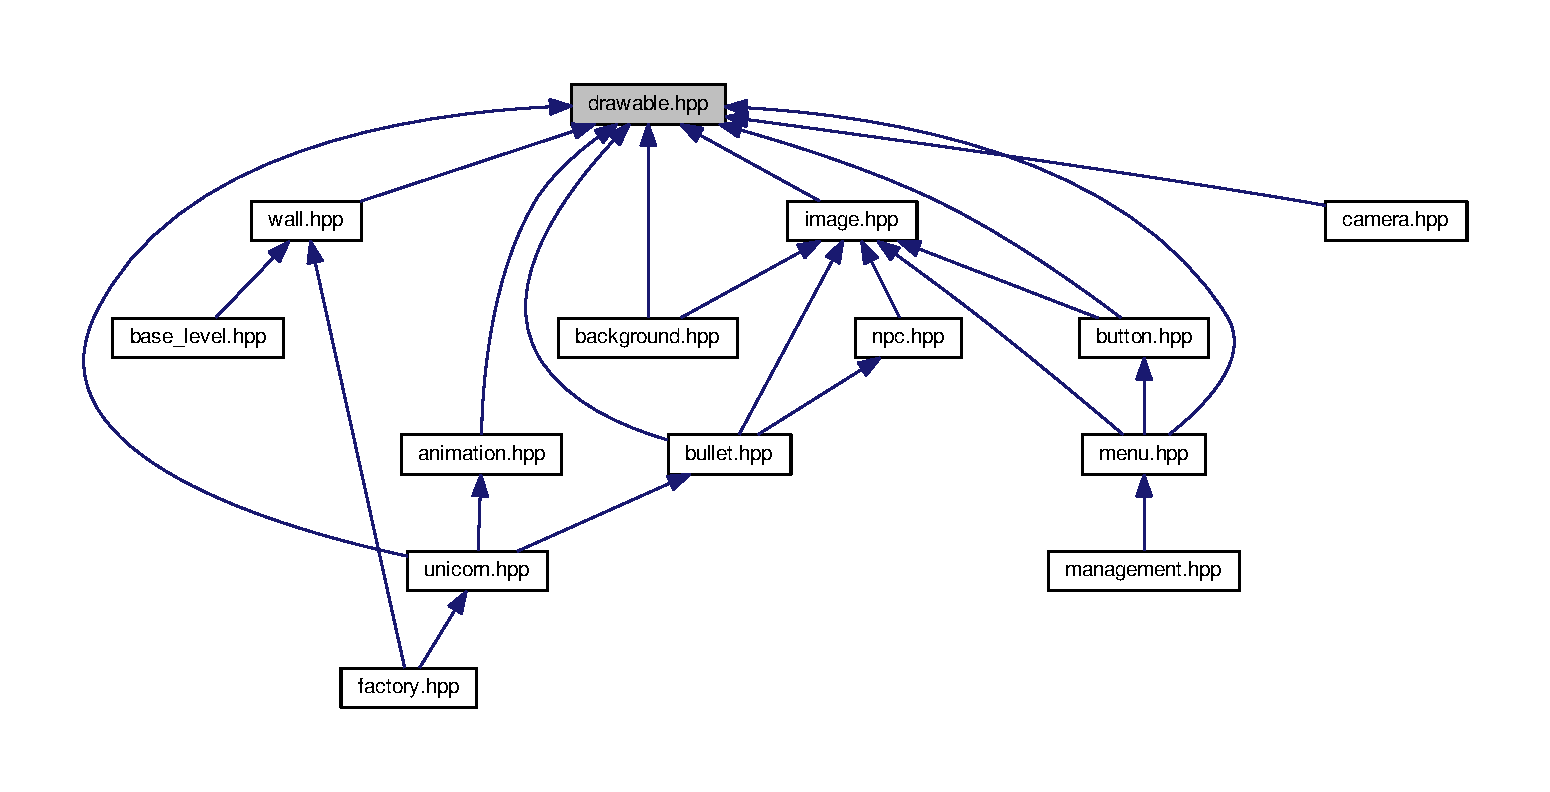
\includegraphics[width=350pt]{drawable_8hpp__dep__incl}
\end{center}
\end{figure}
\subsection*{Classes}
\begin{DoxyCompactItemize}
\item 
struct \hyperlink{structcollision}{collision}
\begin{DoxyCompactList}\small\item\em a collision \end{DoxyCompactList}\item 
class \hyperlink{classaction}{action}
\begin{DoxyCompactList}\small\item\em actions that a charater can do \end{DoxyCompactList}\item 
class \hyperlink{classdrawable}{drawable}
\begin{DoxyCompactList}\small\item\em class that is inherited by all objects that are drawable \end{DoxyCompactList}\end{DoxyCompactItemize}
\subsection*{Typedefs}
\begin{DoxyCompactItemize}
\item 
\mbox{\Hypertarget{drawable_8hpp_aab5add95f06d2ba25dbfed8eb07274fa}\label{drawable_8hpp_aab5add95f06d2ba25dbfed8eb07274fa}} 
typedef std\+::shared\+\_\+ptr$<$ \hyperlink{classdrawable}{drawable} $>$ {\bfseries object\+\_\+ptr}
\item 
\mbox{\Hypertarget{drawable_8hpp_a7e1a7f34f6d09dabb4cdafd6e4118603}\label{drawable_8hpp_a7e1a7f34f6d09dabb4cdafd6e4118603}} 
typedef std\+::vector$<$ \hyperlink{structcollision}{collision} $>$ {\bfseries collisions}
\item 
\mbox{\Hypertarget{drawable_8hpp_a38f93e4749e0d65d51360c429766d212}\label{drawable_8hpp_a38f93e4749e0d65d51360c429766d212}} 
typedef std\+::vector$<$ \hyperlink{classaction}{action} $>$ {\bfseries actions}
\item 
\mbox{\Hypertarget{drawable_8hpp_a6c0fdb1dfd0c34dbbdbb5dcd3c608b07}\label{drawable_8hpp_a6c0fdb1dfd0c34dbbdbb5dcd3c608b07}} 
typedef std\+::vector$<$ object\+\_\+ptr $>$ {\bfseries objects\+\_\+vector}
\end{DoxyCompactItemize}

\hypertarget{exceptions_8hpp}{}\section{exceptions.\+hpp File Reference}
\label{exceptions_8hpp}\index{exceptions.\+hpp@{exceptions.\+hpp}}
This graph shows which files directly or indirectly include this file\+:
\nopagebreak
\begin{figure}[H]
\begin{center}
\leavevmode
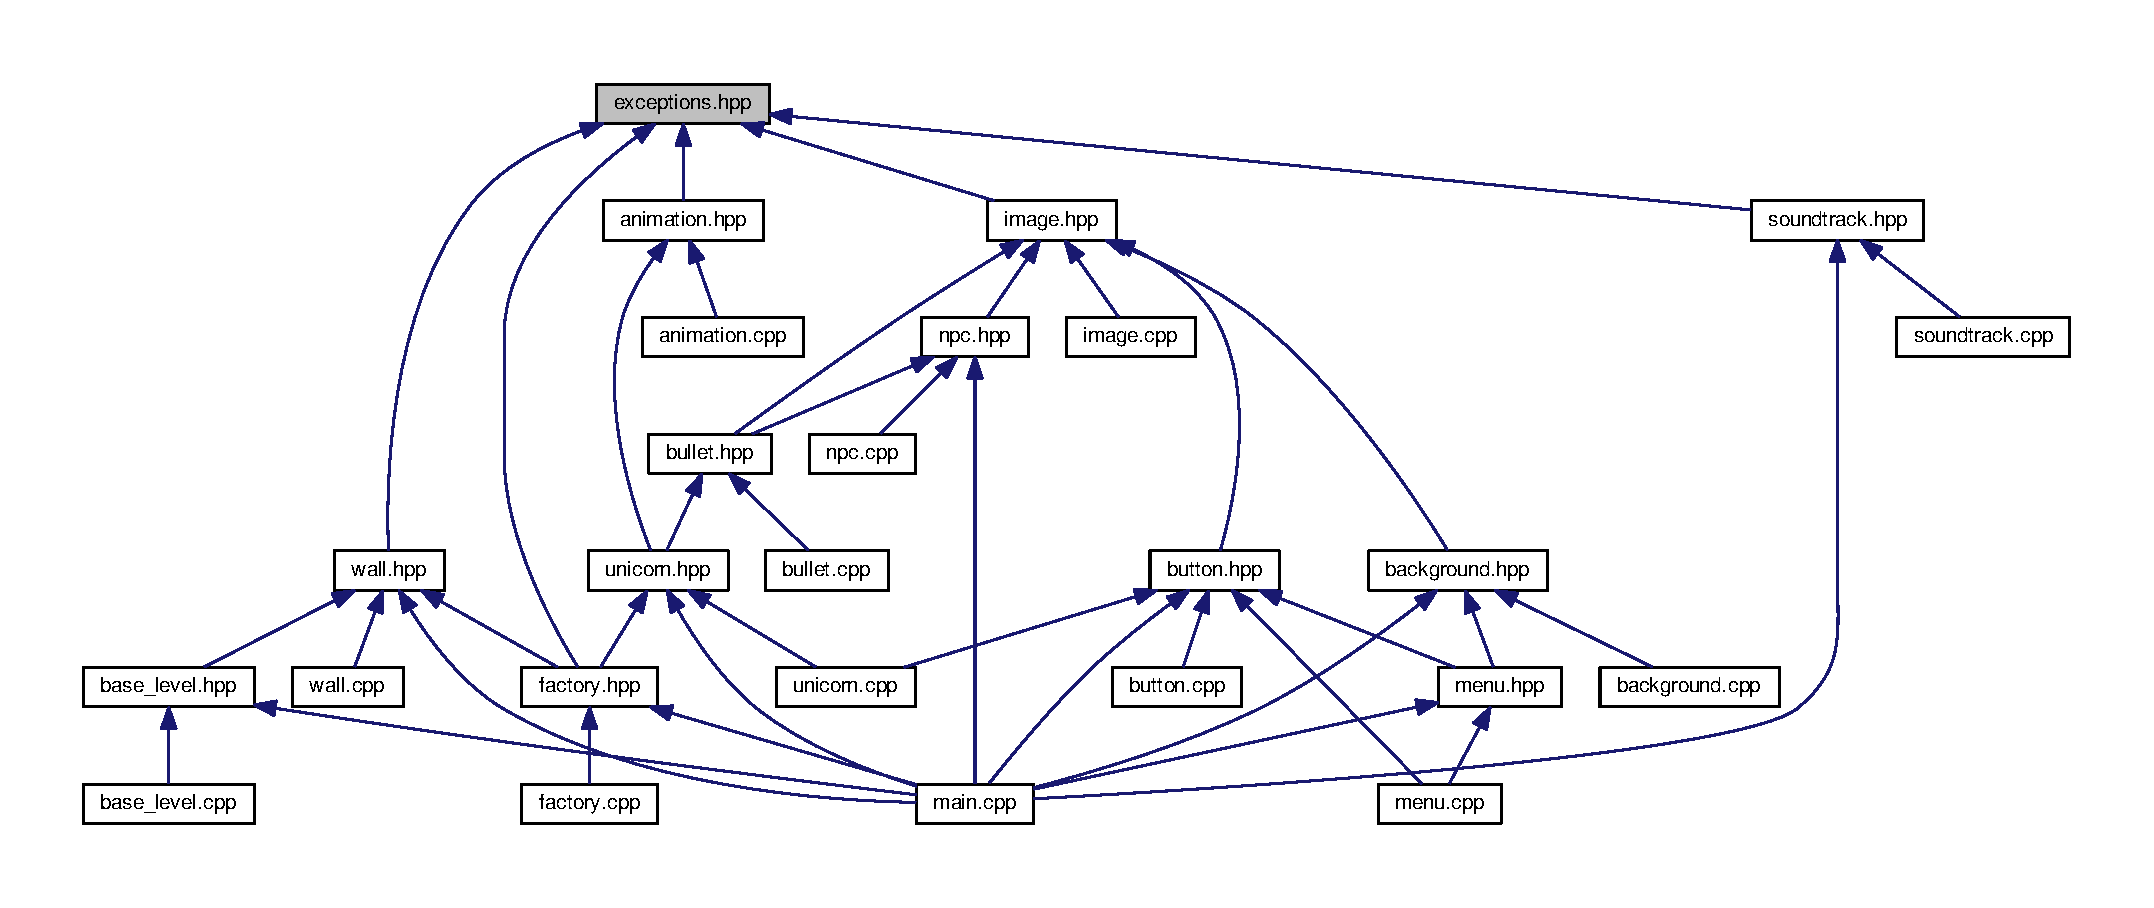
\includegraphics[width=350pt]{exceptions_8hpp__dep__incl}
\end{center}
\end{figure}
\subsection*{Classes}
\begin{DoxyCompactItemize}
\item 
class \hyperlink{classimage__load__error}{image\+\_\+load\+\_\+error}
\begin{DoxyCompactList}\small\item\em image load error \end{DoxyCompactList}\item 
class \hyperlink{classinvalid__position}{invalid\+\_\+position}
\begin{DoxyCompactList}\small\item\em Invalid position exception. \end{DoxyCompactList}\item 
class \hyperlink{classend__of__file}{end\+\_\+of\+\_\+file}
\begin{DoxyCompactList}\small\item\em End of file error. \end{DoxyCompactList}\item 
class \hyperlink{classunknown__color}{unknown\+\_\+color}
\begin{DoxyCompactList}\small\item\em Unknown color error. \end{DoxyCompactList}\item 
class \hyperlink{classunknown__type}{unknown\+\_\+type}
\begin{DoxyCompactList}\small\item\em Unknown type error. \end{DoxyCompactList}\item 
class \hyperlink{classaudio__load__error}{audio\+\_\+load\+\_\+error}
\begin{DoxyCompactList}\small\item\em \hyperlink{classaudio__load__error}{audio\+\_\+load\+\_\+error} \end{DoxyCompactList}\item 
class \hyperlink{classsheet__load__error}{sheet\+\_\+load\+\_\+error}
\begin{DoxyCompactList}\small\item\em sheet load error \end{DoxyCompactList}\end{DoxyCompactItemize}

\hypertarget{factory_8hpp}{}\section{factory.\+hpp File Reference}
\label{factory_8hpp}\index{factory.\+hpp@{factory.\+hpp}}
{\ttfamily \#include \char`\"{}wall.\+hpp\char`\"{}}\\*
{\ttfamily \#include \char`\"{}unicorn.\+hpp\char`\"{}}\\*
{\ttfamily \#include $<$fstream$>$}\\*
Include dependency graph for factory.\+hpp\+:\nopagebreak
\begin{figure}[H]
\begin{center}
\leavevmode
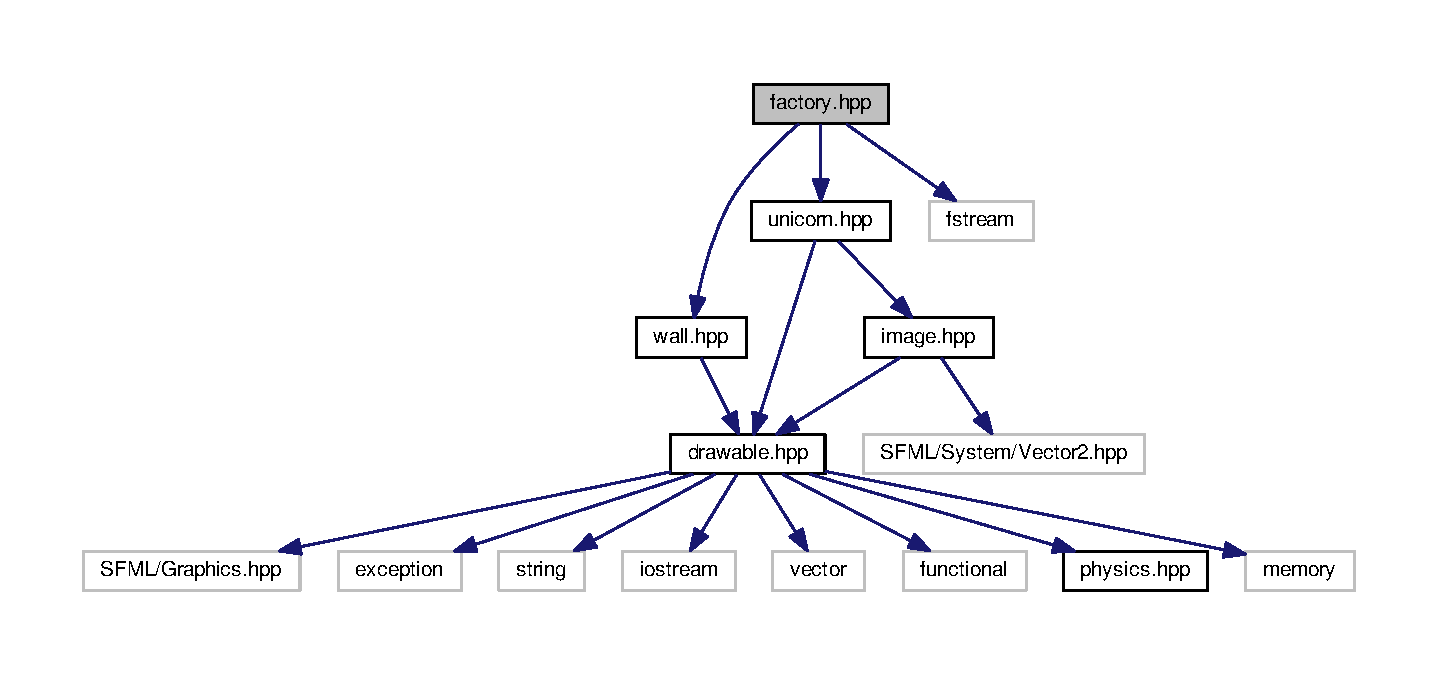
\includegraphics[width=350pt]{factory_8hpp__incl}
\end{center}
\end{figure}
\subsection*{Classes}
\begin{DoxyCompactItemize}
\item 
class \hyperlink{classinvalid__position}{invalid\+\_\+position}
\begin{DoxyCompactList}\small\item\em invalid position exception \end{DoxyCompactList}\item 
class \hyperlink{classend__of__file}{end\+\_\+of\+\_\+file}
\item 
class \hyperlink{classunknown__color}{unknown\+\_\+color}
\item 
class \hyperlink{classunknown__type}{unknown\+\_\+type}
\item 
class \hyperlink{classfactory}{factory}
\end{DoxyCompactItemize}
\subsection*{Functions}
\begin{DoxyCompactItemize}
\item 
std\+::ifstream \& {\bfseries operator$>$$>$} (std\+::ifstream \&input, sf\+::\+Vector2f \&rhs)\hypertarget{factory_8hpp_af8646b44c0d9bcf25ca4064ab22601f8}{}\label{factory_8hpp_af8646b44c0d9bcf25ca4064ab22601f8}

\item 
std\+::ifstream \& {\bfseries operator$>$$>$} (std\+::ifstream \&input, sf\+::\+Color \&rhs)\hypertarget{factory_8hpp_aedc8da7651164363a07b8c75b061b0d8}{}\label{factory_8hpp_aedc8da7651164363a07b8c75b061b0d8}

\end{DoxyCompactItemize}

\hypertarget{image_8hpp}{}\section{image.\+hpp File Reference}
\label{image_8hpp}\index{image.\+hpp@{image.\+hpp}}
{\ttfamily \#include \char`\"{}drawable.\+hpp\char`\"{}}\newline
{\ttfamily \#include \char`\"{}exceptions.\+hpp\char`\"{}}\newline
Include dependency graph for image.\+hpp\+:\nopagebreak
\begin{figure}[H]
\begin{center}
\leavevmode
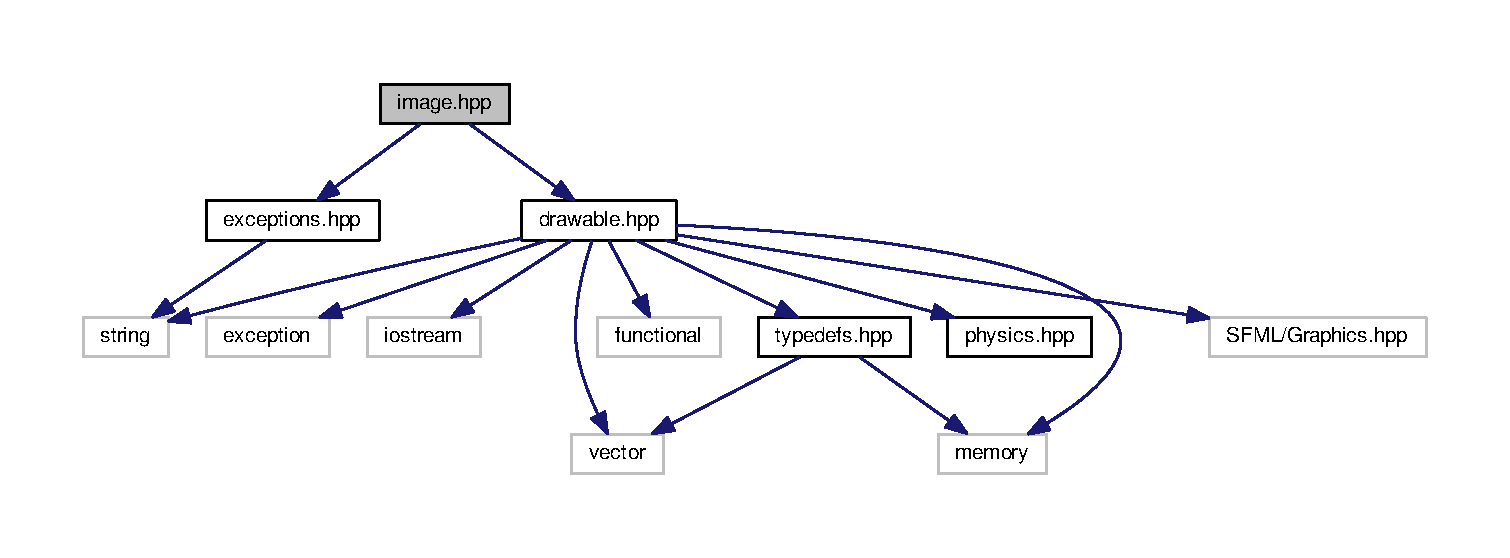
\includegraphics[width=350pt]{image_8hpp__incl}
\end{center}
\end{figure}
This graph shows which files directly or indirectly include this file\+:\nopagebreak
\begin{figure}[H]
\begin{center}
\leavevmode
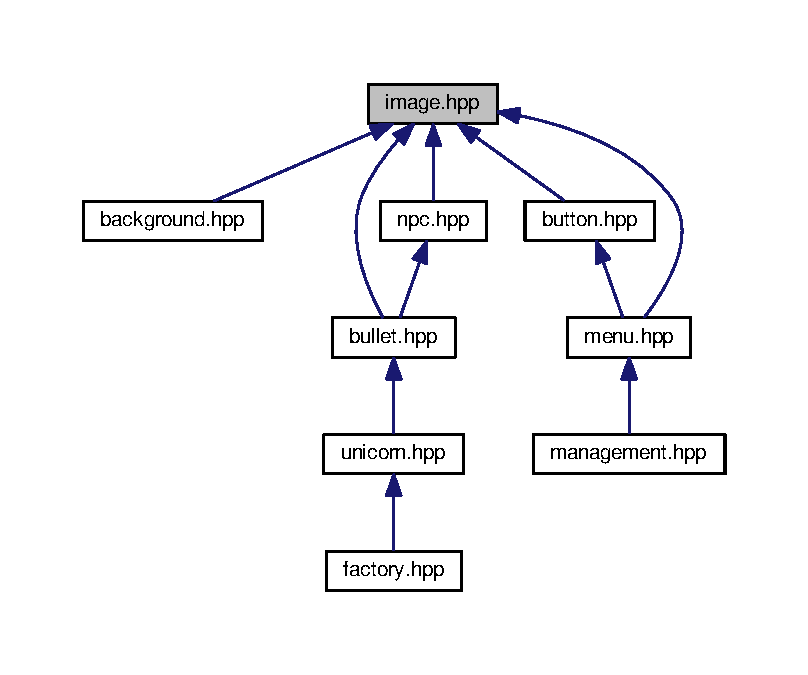
\includegraphics[width=274pt]{image_8hpp__dep__incl}
\end{center}
\end{figure}
\subsection*{Classes}
\begin{DoxyCompactItemize}
\item 
class \hyperlink{classimage__from__file}{image\+\_\+from\+\_\+file}
\begin{DoxyCompactList}\small\item\em create sprite on screen \end{DoxyCompactList}\end{DoxyCompactItemize}

\hypertarget{mainpage_8hpp}{}\section{mainpage.\+hpp File Reference}
\label{mainpage_8hpp}\index{mainpage.\+hpp@{mainpage.\+hpp}}

\hypertarget{management_8hpp}{}\section{management.\+hpp File Reference}
\label{management_8hpp}\index{management.\+hpp@{management.\+hpp}}
{\ttfamily \#include $<$iostream$>$}\newline
{\ttfamily \#include $<$fstream$>$}\newline
{\ttfamily \#include \char`\"{}menu.\+hpp\char`\"{}}\newline
{\ttfamily \#include \char`\"{}cutscene1.\+hpp\char`\"{}}\newline
{\ttfamily \#include \char`\"{}soundtrack.\+hpp\char`\"{}}\newline
Include dependency graph for management.\+hpp\+:
\nopagebreak
\begin{figure}[H]
\begin{center}
\leavevmode
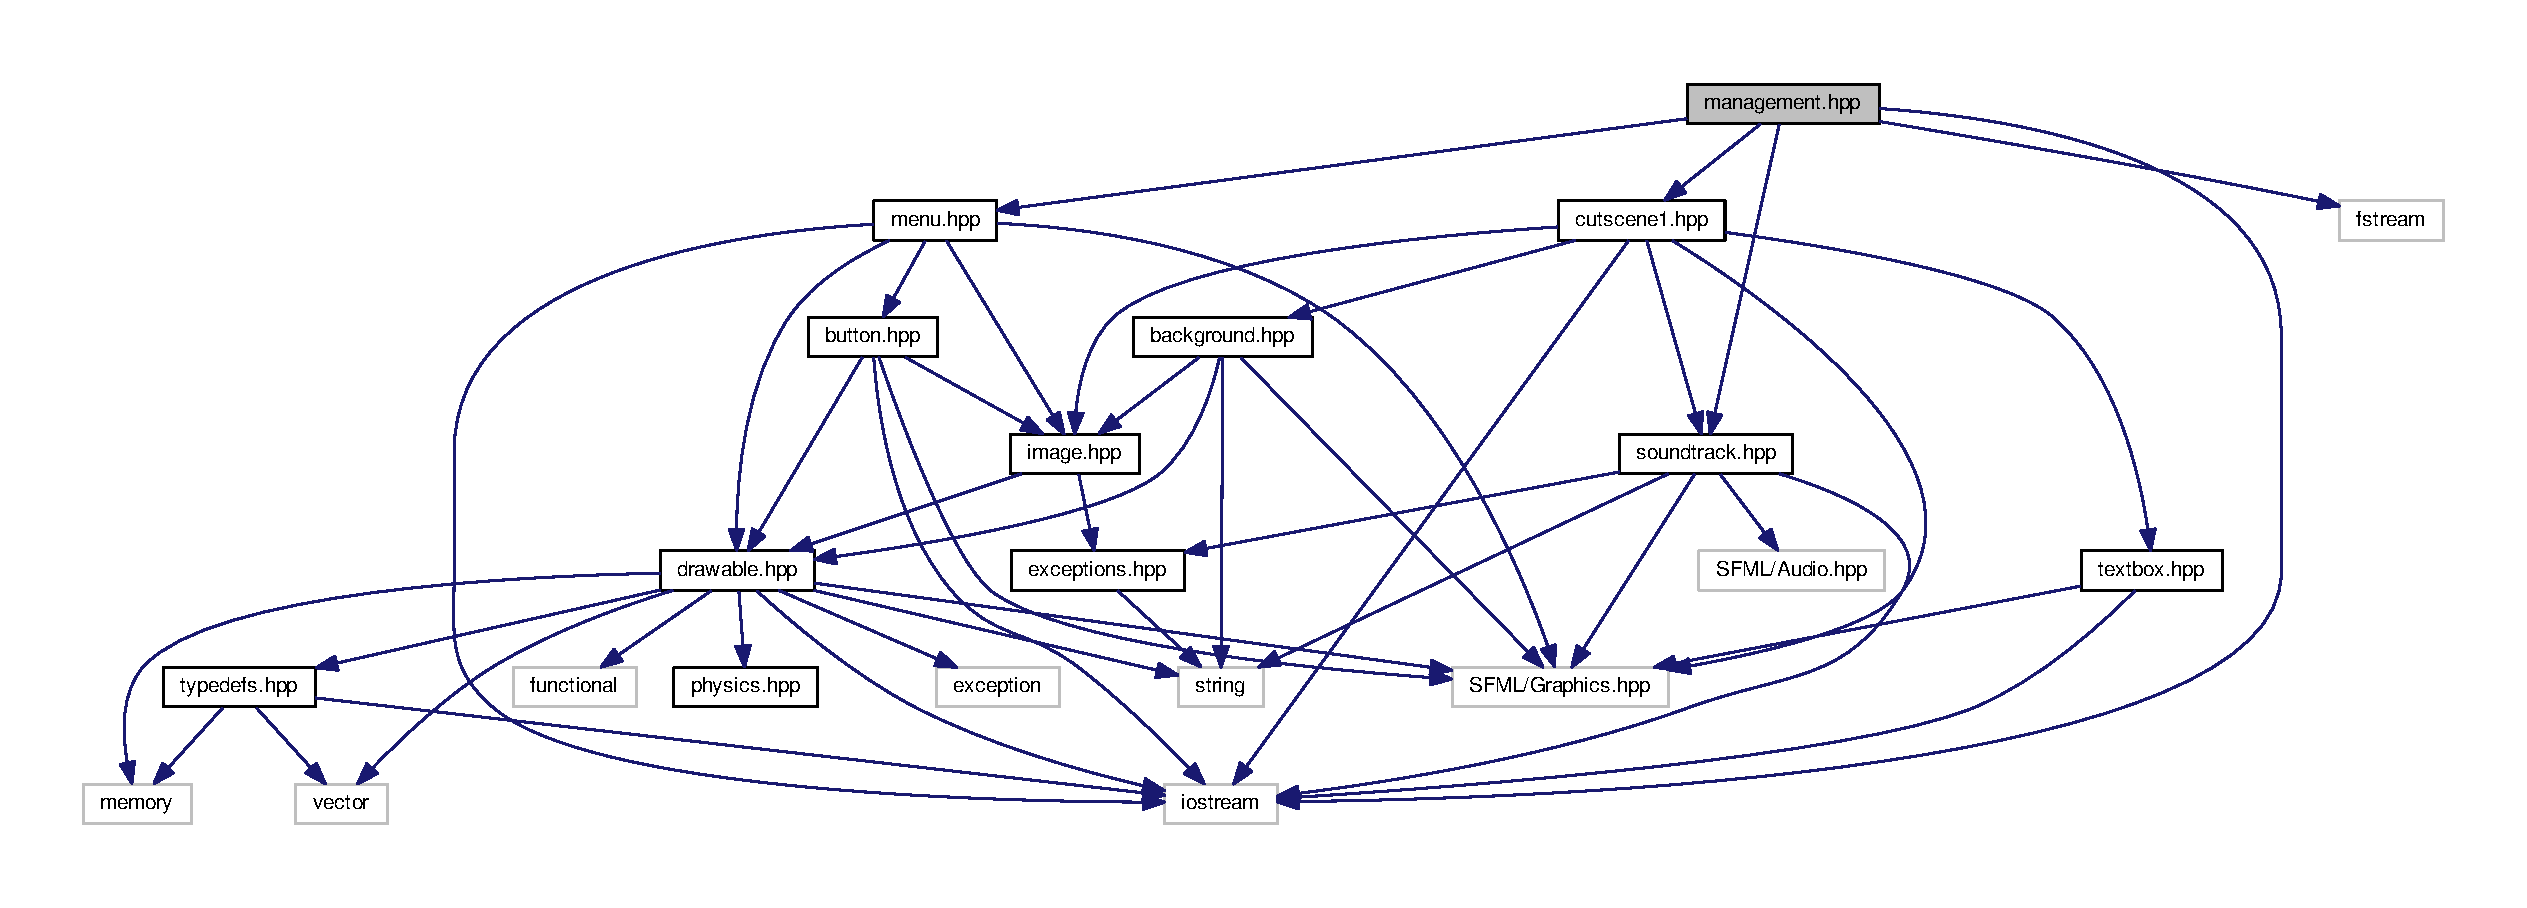
\includegraphics[width=350pt]{management_8hpp__incl}
\end{center}
\end{figure}
\subsection*{Classes}
\begin{DoxyCompactItemize}
\item 
class \hyperlink{classfile__management}{file\+\_\+management}
\begin{DoxyCompactList}\small\item\em file manager for the save-\/files \end{DoxyCompactList}\item 
class \hyperlink{classmenu__management}{menu\+\_\+management}
\begin{DoxyCompactList}\small\item\em manager of all menu\textquotesingle{}s in game \end{DoxyCompactList}\end{DoxyCompactItemize}

\hypertarget{menu_8hpp}{}\section{menu.\+hpp File Reference}
\label{menu_8hpp}\index{menu.\+hpp@{menu.\+hpp}}
{\ttfamily \#include $<$S\+F\+M\+L/\+Graphics.\+hpp$>$}\newline
{\ttfamily \#include $<$iostream$>$}\newline
{\ttfamily \#include \char`\"{}drawable.\+hpp\char`\"{}}\newline
{\ttfamily \#include \char`\"{}image.\+hpp\char`\"{}}\newline
{\ttfamily \#include \char`\"{}button.\+hpp\char`\"{}}\newline
Include dependency graph for menu.\+hpp\+:
\nopagebreak
\begin{figure}[H]
\begin{center}
\leavevmode
\includegraphics[width=350pt]{menu_8hpp__incl}
\end{center}
\end{figure}
This graph shows which files directly or indirectly include this file\+:\nopagebreak
\begin{figure}[H]
\begin{center}
\leavevmode
\includegraphics[width=172pt]{menu_8hpp__dep__incl}
\end{center}
\end{figure}
\subsection*{Classes}
\begin{DoxyCompactItemize}
\item 
class \hyperlink{classmenu}{menu}
\begin{DoxyCompactList}\small\item\em Creates a menu with up to 3 buttons. \end{DoxyCompactList}\end{DoxyCompactItemize}

\hypertarget{npc_8hpp}{}\section{npc.\+hpp File Reference}
\label{npc_8hpp}\index{npc.\+hpp@{npc.\+hpp}}
{\ttfamily \#include \char`\"{}typedefs.\+hpp\char`\"{}}\newline
{\ttfamily \#include \char`\"{}image.\+hpp\char`\"{}}\newline
Include dependency graph for npc.\+hpp\+:
\nopagebreak
\begin{figure}[H]
\begin{center}
\leavevmode
\includegraphics[width=350pt]{npc_8hpp__incl}
\end{center}
\end{figure}
This graph shows which files directly or indirectly include this file\+:\nopagebreak
\begin{figure}[H]
\begin{center}
\leavevmode
\includegraphics[width=147pt]{npc_8hpp__dep__incl}
\end{center}
\end{figure}
\subsection*{Classes}
\begin{DoxyCompactItemize}
\item 
class \hyperlink{classmob}{mob}
\begin{DoxyCompactList}\small\item\em class that makes an enemy to play agianst \end{DoxyCompactList}\end{DoxyCompactItemize}

\hypertarget{physics_8hpp}{}\section{physics.\+hpp File Reference}
\label{physics_8hpp}\index{physics.\+hpp@{physics.\+hpp}}
This graph shows which files directly or indirectly include this file\+:\nopagebreak
\begin{figure}[H]
\begin{center}
\leavevmode
\includegraphics[width=350pt]{physics_8hpp__dep__incl}
\end{center}
\end{figure}
\subsection*{Classes}
\begin{DoxyCompactItemize}
\item 
class \hyperlink{classphysics}{physics}
\begin{DoxyCompactList}\small\item\em Class with physics function. \end{DoxyCompactList}\end{DoxyCompactItemize}

\hypertarget{soundtrack_8hpp}{}\section{soundtrack.\+hpp File Reference}
\label{soundtrack_8hpp}\index{soundtrack.\+hpp@{soundtrack.\+hpp}}
{\ttfamily \#include $<$S\+F\+M\+L/\+Graphics.\+hpp$>$}\newline
{\ttfamily \#include $<$S\+F\+M\+L/\+Audio.\+hpp$>$}\newline
{\ttfamily \#include $<$iostream$>$}\newline
{\ttfamily \#include $<$string$>$}\newline
{\ttfamily \#include \char`\"{}exceptions.\+hpp\char`\"{}}\newline
Include dependency graph for soundtrack.\+hpp\+:\nopagebreak
\begin{figure}[H]
\begin{center}
\leavevmode
\includegraphics[width=350pt]{soundtrack_8hpp__incl}
\end{center}
\end{figure}
\subsection*{Classes}
\begin{DoxyCompactItemize}
\item 
class \hyperlink{classsoundtrack}{soundtrack}
\begin{DoxyCompactList}\small\item\em Class that plays either music or sound effects. \end{DoxyCompactList}\end{DoxyCompactItemize}

\hypertarget{typedefs_8hpp}{}\section{typedefs.\+hpp File Reference}
\label{typedefs_8hpp}\index{typedefs.\+hpp@{typedefs.\+hpp}}
{\ttfamily \#include $<$memory$>$}\newline
{\ttfamily \#include $<$vector$>$}\newline
Include dependency graph for typedefs.\+hpp\+:
\nopagebreak
\begin{figure}[H]
\begin{center}
\leavevmode
\includegraphics[width=194pt]{typedefs_8hpp__incl}
\end{center}
\end{figure}
This graph shows which files directly or indirectly include this file\+:
\nopagebreak
\begin{figure}[H]
\begin{center}
\leavevmode
\includegraphics[width=350pt]{typedefs_8hpp__dep__incl}
\end{center}
\end{figure}
\subsection*{Typedefs}
\begin{DoxyCompactItemize}
\item 
\mbox{\Hypertarget{typedefs_8hpp_aab5add95f06d2ba25dbfed8eb07274fa}\label{typedefs_8hpp_aab5add95f06d2ba25dbfed8eb07274fa}} 
typedef std\+::shared\+\_\+ptr$<$ \hyperlink{classdrawable}{drawable} $>$ \hyperlink{typedefs_8hpp_aab5add95f06d2ba25dbfed8eb07274fa}{object\+\_\+ptr}
\begin{DoxyCompactList}\small\item\em std\+::shared\+\_\+ptr to a \hyperlink{classdrawable}{drawable} object \end{DoxyCompactList}\item 
\mbox{\Hypertarget{typedefs_8hpp_a6c0fdb1dfd0c34dbbdbb5dcd3c608b07}\label{typedefs_8hpp_a6c0fdb1dfd0c34dbbdbb5dcd3c608b07}} 
typedef std\+::vector$<$ \hyperlink{typedefs_8hpp_aab5add95f06d2ba25dbfed8eb07274fa}{object\+\_\+ptr} $>$ \hyperlink{typedefs_8hpp_a6c0fdb1dfd0c34dbbdbb5dcd3c608b07}{objects\+\_\+vector}
\begin{DoxyCompactList}\small\item\em std\+::vector with \hyperlink{typedefs_8hpp_aab5add95f06d2ba25dbfed8eb07274fa}{object\+\_\+ptr} objects \end{DoxyCompactList}\item 
\mbox{\Hypertarget{typedefs_8hpp_a7e1a7f34f6d09dabb4cdafd6e4118603}\label{typedefs_8hpp_a7e1a7f34f6d09dabb4cdafd6e4118603}} 
typedef std\+::vector$<$ \hyperlink{structcollision}{collision} $>$ \hyperlink{typedefs_8hpp_a7e1a7f34f6d09dabb4cdafd6e4118603}{collisions}
\begin{DoxyCompactList}\small\item\em std\+::vector with \hyperlink{structcollision}{collision} objects \end{DoxyCompactList}\item 
\mbox{\Hypertarget{typedefs_8hpp_a38f93e4749e0d65d51360c429766d212}\label{typedefs_8hpp_a38f93e4749e0d65d51360c429766d212}} 
typedef std\+::vector$<$ \hyperlink{classaction}{action} $>$ \hyperlink{typedefs_8hpp_a38f93e4749e0d65d51360c429766d212}{actions}
\begin{DoxyCompactList}\small\item\em std\+::vector with \hyperlink{classaction}{action} objects \end{DoxyCompactList}\item 
\mbox{\Hypertarget{typedefs_8hpp_a09ee7f853fc9bc830a9445a06fd53d4b}\label{typedefs_8hpp_a09ee7f853fc9bc830a9445a06fd53d4b}} 
typedef std\+::shared\+\_\+ptr$<$ \hyperlink{classmob}{mob} $>$ \hyperlink{typedefs_8hpp_a09ee7f853fc9bc830a9445a06fd53d4b}{mob\+\_\+ptr}
\begin{DoxyCompactList}\small\item\em std\+::shared\+\_\+ptr with \hyperlink{classmob}{mob} objects \end{DoxyCompactList}\end{DoxyCompactItemize}

\hypertarget{unicorn_8hpp}{}\section{unicorn.\+hpp File Reference}
\label{unicorn_8hpp}\index{unicorn.\+hpp@{unicorn.\+hpp}}
{\ttfamily \#include \char`\"{}drawable.\+hpp\char`\"{}}\newline
{\ttfamily \#include \char`\"{}animation.\+hpp\char`\"{}}\newline
{\ttfamily \#include $<$iostream$>$}\newline
{\ttfamily \#include \char`\"{}bullet.\+hpp\char`\"{}}\newline
Include dependency graph for unicorn.\+hpp\+:
\nopagebreak
\begin{figure}[H]
\begin{center}
\leavevmode
\includegraphics[width=350pt]{unicorn_8hpp__incl}
\end{center}
\end{figure}
This graph shows which files directly or indirectly include this file\+:
\nopagebreak
\begin{figure}[H]
\begin{center}
\leavevmode
\includegraphics[width=147pt]{unicorn_8hpp__dep__incl}
\end{center}
\end{figure}
\subsection*{Classes}
\begin{DoxyCompactItemize}
\item 
class \hyperlink{classunicorn}{unicorn}
\begin{DoxyCompactList}\small\item\em class that is used to display and control the unicorn \end{DoxyCompactList}\end{DoxyCompactItemize}

\hypertarget{wall_8hpp}{}\section{wall.\+hpp File Reference}
\label{wall_8hpp}\index{wall.\+hpp@{wall.\+hpp}}
{\ttfamily \#include \char`\"{}drawable.\+hpp\char`\"{}}\newline
{\ttfamily \#include \char`\"{}exceptions.\+hpp\char`\"{}}\newline
Include dependency graph for wall.\+hpp\+:
\nopagebreak
\begin{figure}[H]
\begin{center}
\leavevmode
\includegraphics[width=350pt]{wall_8hpp__incl}
\end{center}
\end{figure}
This graph shows which files directly or indirectly include this file\+:\nopagebreak
\begin{figure}[H]
\begin{center}
\leavevmode
\includegraphics[width=246pt]{wall_8hpp__dep__incl}
\end{center}
\end{figure}
\subsection*{Classes}
\begin{DoxyCompactItemize}
\item 
class \hyperlink{classwall}{wall}
\begin{DoxyCompactList}\small\item\em Class for walls and platforms. \end{DoxyCompactList}\end{DoxyCompactItemize}

%--- End generated contents ---

% Index
\backmatter
\newpage
\phantomsection
\clearemptydoublepage
\addcontentsline{toc}{chapter}{Index}
\printindex

\end{document}
